\chapter{Early Stopping Score Matching Density Estimator}
\label{ch3}


In this chapter, we introduce the early stopping SM density estimator and discuss its statistical properties. As we have discussed in Chapter \ref{ch2}, minimizing $\widehat{J}_{\SM}$ over $\calH$ has no solution and a certain kind of regularization has to be imposed. The approach adopted by \textcite{Sriperumbudur-density-estimation-inf-exp-family} was to add a penalty functional and minimize the penalized SM loss functional, which yields the penalized SM density estimator. In this chapter, we consider the early stopping approach to regularize. More precisely, we apply the gradient descent algorithm to minimizing $\widehat{J}_{\SM}$ and terminate the algorithm early, leading to the early stopping SM density estimator. 

After an overview of the early stopping regularization and the gradient descent algorithm in Section \ref{section-gd-overview}, we present our early stopping SM density estimator in Section \ref{section-smes-estimator}. We then study its theoretical properties in Section \ref{section-theoretical-properties}. Finally, we compare our early stopping SM density estimator with the penalized SM density estimator in Section \ref{section-compare-smes-smpen}. 

\section{An Overview} \label{section-gd-overview}

Early stopping is a form of regularization based on choosing when to terminate an iterative optimization algorithm. This form of regularization is often referred to as implicit regularization, in contrast to the penalized approach by explicitly adding a penalty term. %The main advantage of early stopping regularization, compared with the penalized approach, is the lower computational complexity. 

In the supervised learning setting where a model is estimated via minimizing a loss function, using early stopping can effectively avoid overfitting so that the resulting estimated model can generalize well. It is essentially a bias-variance tradeoff: stopping the algorithm too early results in a model with a large bias and a small variance, but stopping it too late leads to a model with a small bias but a large variance. Stopping the algorithm early (but not too early) is an approach to solve this bias-variance tradeoff. Early stopping has been systematically investigated in $L_2$ boosting algorithm \parencite{Buhlmann2003-dk}, boosting algorithm for a general convex loss function \parencite{Zhang2005-pi}, and the nonparametric least squares regression in the RKHS setting \parencite{Yao2007-ji,Raskutti14-dw}, to name a few. 

In our development below, we choose the iterative optimization algorithm to be the gradient descent algorithm, which is a first-order optimization algorithm for solving an unconstrained minimization problem. Starting from a point in the feasible set, at each iteration, the gradient descent algorithm goes along the direction of the negative gradient of the objective function at the current point. This direction is the one with the steepest descent. 

Mathematically, let $g: \Real^m \to \Real$ be a convex differentiable function and assume there exists a unique $x^* \in \Real^m$ such that $\inf_{x \in \Real^m} g \parens{x} = g \parens{x^*} > -\infty$. We would like to minimize $g$ over $\Real^m$. Gradient descent algorithm starts from $x^{\parens{0}} \in \Real^m$ and generates the sequence 
\begin{align*}
	x^{\parens{t+1}} = x^{\parens{t}} - \tau_t \nabla g \parens{x^{\parens{t}}}, \qquad \qquad \text{ for all } t \in \Natural_0 := \Natural \cup \sets{0}, 
\end{align*}
where $\tau_t > 0$ is the appropriately chosen step size and the subscript ``$t$'' indicates that the step size may differ for different numbers of iterations. With appropriately chosen $\sets{\tau_t}_{t \in \Natural}$, the gradient descent algorithm guarantees $g$ is decreased at each iteration, i.e., $g \parens{x^{\parens{t+1}}} < g \parens{x^{\parens{t}}}$ for all $t \in \Natural_0$, except when $g$ has already achieved the minimum at $x^{\parens{t}}$. One terminates the algorithm when one of the following three criteria does not exceed a pre-specified tolerant parameter
\begin{align*}
	\norm{\nabla g \parens{x^{\parens{t}}}}, \qquad 
	\abs{g \parens{x^{\parens{t+1}}} - g \parens{x^{\parens{t}}}}, \qquad \text{ and } \qquad 
	\abs[\bigg]{\frac{g \parens{x^{\parens{t+1}}} - g \parens{x^{\parens{t}}}}{g \parens{x^{\parens{t}}}} }, 
\end{align*}
where $\norm{\,\cdot\,}$ is a norm over $\Real^m$ chosen by the user. It can be shown that, with appropriately chosen $\sets{\tau_t}_{t \in \Natural}$, the sequence $\sets{g \parens{x^{\parens{t}}}}_{t \in \Natural}$ is guaranteed to converge to $g \parens{x^*}$ as $t \to \infty$ \parencites[see, for example, Chapter 9 in][]{Boyd2004-gi}. 

%Gradient descent method has found a wide range of applications in statistical estimation. We provide one example here. 
%
%\begin{example}[Least Squares Regression]
%	In the least squares regression, we assume the response variable $Y \in \Real$ and the covariate $X \in \Real^d$ are related by the model 
%	\begin{align}
%		Y = X^\top \beta^* + \varepsilon, 
%	\end{align}
%	where $\beta^* \in \Real^d$ is the true coefficient and $\varepsilon \sim \Normal \parens{0, \sigma^2}$ with $\sigma^2 > 0$ being unknown. Let $\sets{\parens{Y_i, X_i}}_{i=1}^n$ are $n$ i.i.d observations, where we assume $n > d$. We estimate $\beta^* := \parens{\beta_1^*, \cdots, \beta_d^*}^\top \in \Real^d$ using the least squares method, which amounts to minimizing 
%	\begin{align}\label{eq-least-squares-regression}
%		\frac{1}{2} \norm{\bY - \bX \beta}_2^2, 
%	\end{align}
%	where $\bY := \parens{Y_1, \cdots, Y_n}^\top \in \Real^n$ and $\bX \in \Real^{n \times d}$ is the design matrix with each row corresponding to an observation and each column corresponding to a covariate. We assume that the matrix $\bX$ is of full rank. 
%	
%	The problem of minimizing \eqref{eq-least-squares-regression} has an analytic solution given by 
%	\begin{align}\label{eq-least-square-inverse}
%		\hat{\beta} := \parens{\bX^\top \bX}^{-1} \bX^\top \bY, 
%	\end{align}
%	where $\parens{\bX^\top \bX}^{-1}$ exists since $\bX$ has full rank. Note that to compute \eqref{eq-least-square-inverse} requires to compute $\parens{\bX^\top \bX}^{-1}$, which requires elementary operations of order $\calO \parens{p^3}$. If $p$ is large, the computation is expensive. 
%	
%	We could also minimize \eqref{eq-least-squares-regression} using the gradient descent algorithm. Starting from $\beta^{\parens{0}}$, the gradient descent iterates are given by 
%	\begin{align*}
%		\beta^{\parens{t+1}} = \beta^{\parens{t}} - \tau \bX^\top \parens{\bX \beta^{\parens{t}} - \bY}, \qquad \text{ for all } t \in \Natural_0 := \Natural \cup \sets{0}, 
%	\end{align*}
%	where $\tau > 0$ is the constant step size. We terminate the algorithm when $\norm{\bX^\top \parens{\bX \beta^{\parens{t}} - \bY}} \le \gamma$, where $\gamma > 0$ is a pre-specified positive constant. With an appropriate $\tau$, computing $\beta^{\parens{t}}$ only requires elementary operations of order $\calO \parens{p^2 n}$. From here, we see the computational advantage of using the gradient descent algorithm over working with the analytic solution directly using \eqref{eq-least-square-inverse}. 
%\end{example}

\section{Early Stopping Score Matching Density Estimator}\label{section-smes-estimator}

We present our early stopping SM density estimator in this section. %, which is obtained by applying the gradient descent algorithm to minimizing $\widehat{J}_{\SM}$ over $\calH$ and terminating the algorithm early. 

To start with, we formally state a set of assumptions, in addition to \ref{assumption-2-1-inf-dim} - \ref{assumption-2-4-base-density} in Chapter \ref{ch2}, that will be used. 

\begin{enumerate}[label=\textbf{(B\arabic*)},series=assumptions]
	\item \label{assumption-1} $\calX$ is a non-empty open subset of $\Real^d$ with a piecewise smooth boundary $\partial \calX := \overline{\calX} \backslash \calX$, where $\overline{\calX}$ denotes the closure of $\calX$. 
	\item \label{assumption-2} $p_0$ is continuously differentiable, is continuously extendible to $\overline{\calX}$, and satisfies $\int_{\calX} p_0 \parens{x} \norm{\nabla \log p_0 \parens{x}}_2^2 \diff x < \infty$. 
	\item \label{assumption-3} $k$ is twice continuously differentiable on $\calX \times \calX$ with continuous extension of $\partial_u \partial_{u+d} k$ and $\partial_u \partial_v \partial_{u+d} \partial_{v+d} k$ to $\overline{\calX} \times \overline{\calX}$ for all $u, v = 1, 2, \cdots, d$. 
	\item \label{assumption-4} As $x \to \partial \calX$, $\sup_{u = 1, \cdots, d} \partial_u \partial_{u+d} k \parens{x, x} p_0 \parens{x} \to 0$.  
	\item \label{assumption-5} $\kappa_2 := \sup_{u = 1, \cdots, d} \sup_{x \in \calX} \sqrt{\partial_u \partial_{u+d} k \parens{x, x}} < \infty$, \\ 
		$\kappa_3 := \sup_{u = 1, \cdots, d} \sup_{x \in \calX} \sqrt{\partial_u^2 \partial_{u+d}^2 k \parens{x, x}} < \infty$, and \\ 
		$\kappa_4 := \sup_{u = 1, \cdots, d} \sup_{x \in \calX} \abs{\partial_u \log \mu \parens{x}} \sqrt{\partial_u \partial_{u+d} k \parens{x, x}}  < \infty$. 
\end{enumerate}

Under these assumptions, we can derive the H-divergence between $p_0$ and $q_f \in \calQ_{\ker}$ and the corresponding SM matching loss that we have seen in Chapter \ref{ch2}. 

\begin{theorem}[Theorem 4 in \textcite{Sriperumbudur-density-estimation-inf-exp-family}]\label{thm-smloss} \leavevmode
\begin{enumerate}[label=(\alph*)]
	\item Under \ref{assumption-2-1-inf-dim} - \ref{assumption-2-4-base-density} in Chapter \ref{ch2} and \ref{assumption-1} - \ref{assumption-5} above, the H-divergence between $p_0$ and $q_f \in \calQ_{\kef}$ is 
	\begin{align*}
		J_{\SM} \parens{f} := \frac{1}{2} \innerp{f}{C f}_{\calH} - \innerp{f}{z}_{\calH} + \mathrm{const}, 
	\end{align*}
	where $C: \calH \to \calH$ is a linear positive semidefinite operator given by 
	\begin{align}\label{eq-C-def}
		C := \int_{\calX} p_0 \parens{x} \sum_{u=1}^d \partial_u k \parens{x, \,\cdot\,} \otimes \partial_u k \parens{x, \,\cdot\,} \diff x
	\end{align}
	satisfying $C f = \int_{\calX} p_0 \parens{x} \sum_{u=1}^d \partial_u f \parens{x} \partial_u k \parens{x, \,\cdot\,} \diff x$ for all $f \in \calH$, and $z: \calX \to \Real$ is a function in $\calH$ given by 
	\begin{align}\label{eq-z-def}
		z := - \int_{\calX} p_0 \parens{x} \sum_{u=1}^d \parens[\Big]{\partial^2_u k \parens{x, \,\cdot\,} + \partial_u \log \mu \parens{x} \partial_u k \parens{x, \,\cdot\,}} \diff x, 
	\end{align}
	and const is a term that does \emph{not} depend on $f$ and is equal to $\frac{1}{2} \int_{\calX} p_0 \parens{x} \norm[\big]{\nabla \log p_0 \parens{x} - \nabla \log \mu \parens{x}}_2^2 \diff x$. 
	
	\item Let $X_1, \cdots, X_n$ be i.i.d samples from $p_0$. Under \ref{assumption-2-1-inf-dim} - \ref{assumption-2-4-base-density} in Chapter \ref{ch2}, \ref{assumption-1} - \ref{assumption-5} above, and $q_f \in \calQ_{\kef}$, the SM loss functional is $\widehat{J}_{\SM}: \calH \to \Real$ given by 
	\begin{equation*}% \label{eq-smloss}
		\widehat{J}_{\SM} \parens{f} := \frac{1}{2} \langle f, \widehat{C} f \rangle_{\mathcal{H}} - \langle f, \hat{z} \rangle_{\mathcal{H}} + \mathrm{const}, \qquad \text{ for all } f \in \calH, 
	\end{equation*}
	where $\widehat{C}: \calH \to \calH$ and $\hat{z} \in \calH$ are given by \eqref{eq-hatC} and \eqref{eq-hatz} in Chapter \ref{ch2}, respectively.  
%	\begin{align}\label{eq-hatC-def}
%		\widehat{C} := \frac{1}{n} \sum_{i=1}^n \sum_{u=1}^d \partial_u k \parens{X_i, \,\cdot\,} \otimes \partial_u k \parens{X_i, \,\cdot\,}
%	\end{align}
%	with
%	\begin{align}
%		\widehat{C} f =  \frac{1}{n} \sum_{i=1}^n \sum_{u=1}^d \partial_u f \parens{X_i} \partial_u k \parens{X_i, \,\cdot\,} \quad \text{ for all } f \in \calF, 
%	\end{align}
%	and 
%	\begin{align}\label{hatz.def}
%		\hat{z} := -\frac{1}{n} \sum_{i=1}^n \sum_{u=1}^d \parens[\Big]{\partial^2_u k \parens{X_i, \,\cdot\,} + \partial_u \log \mu \parens{X_i} \partial_u k \parens{X_i, \,\cdot\,}} \in \calH, 
%	\end{align}
%	and const is given by \eqref{eq-T-term} and does not depend on $f$. 
\end{enumerate}
\end{theorem}

The proof of this theorem can be found in \textcite{Sriperumbudur-density-estimation-inf-exp-family} and is omitted here. 

%In order to prove Theorem \ref{thm-smloss}, we need the following lemma from \textcite{Zhou2008-jt}. 
%
%\begin{lemma}[Properties of partial derivatives of kernel function]\label{lemma-zhou-theorem}
%	Assume $k: \calX \times \calX \to \Real$ is twice continuously differentiable over $\calX$. Let $x \in \calX$ and $u \in \sets{1, \cdots, d}$. Then, 
%	\begin{enumerate}[label=(\alph*)]
%		\item both $\partial_u k \parens{x, \,\cdot\,}$ and $\partial_u^2 k \parens{x, \,\cdot\,}$ belong to $\calH$, and 
%		\item for any $f \in \calH$, 
%		\begin{align}
%		  \partial_u f \parens{x} = & \, \innerp{f}{\partial_u k \parens{x, \,\cdot\,}}_{\calH}, \qquad \text{ and } \qquad \partial_u^2 f \parens{x} = \innerp{f}{\partial_u^2 k \parens{x, \,\cdot\,}}_{\calH}, 
%		\end{align}
%		where $\partial_u f$ and $\partial_u^2 f$ denote the first- and second-order partial derivatives of $f$ with respect to the $u$-th coordinate, respectively. 
%	\end{enumerate}
%\end{lemma}
%
%Now, we are ready to prove Theorem \ref{thm-smloss}. 
%
%\begin{proof}[Proof of Theorem \ref{thm-smloss}]
%	(a) By the definition of the H-divergence, we have 
%	\begin{align}
%		\Hdiv \parens{p_0 \Vert q_f} := & \, \frac{1}{2} \int_{\calX} p_0 \parens{x} \norm[\big]{\nabla \log p_0 \parens{x} - \nabla \log q_f \parens{x}}_2^2 \diff x \nonumber \\
%		= & \, \frac{1}{2} \int_{\calX} p_0 (x) \parens[\Big]{\norm{\nabla \log q_f \parens{x}}_2^2 - 2 \innerp[\big]{\nabla \log p_0 \parens{x}}{\nabla \log q_f \parens{x}} + \norm{\nabla \log p_0 \parens{x}}_2^2} \diff x, \label{eq-29}
%	\end{align}
%	where $\nabla \log p \parens{x} := \parens[\big]{\partial_1 \log p \parens{x}, \cdots, \partial_d \log p \parens{x}}^\top \in \Real^d$ and $\partial_u \log p \parens{x} := \frac{\partial \log p \parens{w}}{\partial w_u} \Big\vert_{w = x}$ for $w = \parens{w_1, \cdots, w_d} \in \calX$ and all $u = 1, \cdots, d$. In \eqref{eq-29}, $\innerp{\,\cdot\,}{\,\cdot\,}$ denotes the usual dot product in $\Real^d$ and $\norm{\,\cdot\,}_2$ denotes the Euclidean norm in $\Real^d$. 
%	
%	First note that $\int_{\calX} p_0 \parens{x} \norm{\nabla \log p_0 \parens{x}}_2^2 \diff x$ does not depend on $f$ and is finite by \ref{assumption-2}. 
%	
%	Since $\nabla \log q_f \parens{x} = \nabla \log \mu \parens{x} + \nabla f \parens{x}$, we have 
%	\begin{align*}
%		  \int_{\calX} p_0 \parens{x} \norm[\big]{\nabla \log q_f \parens{x}}_2^2 \diff x 
%		% = & \, \int_{\calX} p_0 \parens{x} \sum_{u=1}^d \parens[\big]{\partial_u \log \mu \parens{x} + \partial_u f \parens{x}}^2 \diff x \\ 
%		= & \, \int_{\calX} p_0 \parens{x} \sum_{u=1}^d \parens[\big]{\partial_u \log \mu \parens{x}}^2 \diff x + 2 \int_{\calX} p_0 \parens{x} \sum_{u=1}^d \partial_u \log \mu \parens{x} \partial_u f \parens{x} \diff x \\ 
%		  & \qquad \qquad + \int_{\calX} p_0 \parens{x} \sum_{u=1}^d \parens[\big]{\partial_u f \parens{x}}^2 \diff x \\
%		\stackrel{\text{(i)}}{=} & \, \int_{\calX} p_0 \parens{x} \norm[\big]{\nabla \log \mu \parens{x}}_2^2 \diff x  + 2 \int_{\calX} p_0 \parens{x} \sum_{u=1}^d \partial_u \log \mu \parens{x} \innerp{f}{\partial_u k \parens{x, \cdot}}_{\calH} \diff x \\ 
%		  & \qquad + \int_{\calX} p_0 \parens{x} \sum_{u=1}^d \innerp[\big]{f}{\parens[\big]{\partial_u k \parens{x, \cdot} \otimes \partial_u k \parens{x, \cdot}} f}_{\calH} \diff x, \\
%		\stackrel{\text{(ii)}}{=} & \, \int_{\calX} p_0 \parens{x} \norm[\big]{\nabla \log \mu \parens{x}}_2^2 \diff x + \innerp[\bigg]{f}{2 \int_{\calX} p_0 \parens{x} \sum_{u=1}^d \partial_u \log \mu \parens{x} \partial_u k \parens{x, \cdot} \diff x}_{\calH} \\ 
%		  & \qquad + \innerp[\bigg]{f}{\parens[\bigg]{\int_{\calX} p_0 \parens{x} \sum_{u=1}^d \partial_u k \parens{x, \cdot} \otimes \partial_u k \parens{x, \cdot} \diff x} f}_{\calH}, 
%	\end{align*}
%	where we use Lemma \ref{lemma-zhou-theorem} and $\innerp{a}{b}_{\calH}^2 = \innerp{a}{b}_{\calH} \innerp{a}{b}_{\calH} = \innerp{a}{\parens{b \otimes b} a}_{\calH}$, for $a, b \in \calH$, in (i), and swap the integral and the inner product in (ii) using \ref{assumption-6}. 
%	
%	As for $\int_{\calX} p_0 \parens{x} \innerp{\nabla \log p_0 \parens{x}}{\nabla \log q_f \parens{x}} \diff x$ in \eqref{eq-29}, we have 
%	\begin{align*}
%		& \, \int_{\calX} p_0 \parens{x} \innerp[\big]{\nabla \log p_0 \parens{x}}{\nabla \log q_f \parens{x}} \diff x \\ 
%		= & \, \int_{\calX} p_0 \parens{x} \innerp[\big]{\nabla \log p_0 \parens{x}}{\nabla \log \mu \parens{x}} \diff x + \sum_{u=1}^d \int_{\calX} p_0 \parens{x} \frac{\partial_u p_0 \parens{x}}{p_0 \parens{x}} \partial_u f \parens{x} \diff x \\ 
%	 	= & \, \int_{\calX} p_0 \parens{x} \innerp[\big]{\nabla \log p_0 \parens{x}}{\nabla \log \mu \parens{x}} \diff x + \sum_{u=1}^d \int_{\calX} \partial_u p_0 \parens{x} \partial_u f \parens{x} \diff x \\ 
%		\stackrel{\text{(iii)}}{=} & \, \int_{\calX} p_0 \parens{x} \innerp[\big]{\nabla \log p_0 \parens{x}}{\nabla \log \mu \parens{x}} \diff x - \sum_{u=1}^d \int_{\calX} p_0 \parens{x} \partial_u^2 f \parens{x} \diff x \\
%		\stackrel{\text{(iv)}}{=} & \, \int_{\calX} p_0 \parens{x} \innerp[\big]{\nabla \log p_0 \parens{x}}{\nabla \log \mu \parens{x}} \diff x - \innerp[\bigg]{f}{\int_{\calX} p_0 \parens{x} \sum_{u=1}^d \partial_u^2 k \parens{x, \cdot} \diff x}_{\calH}, 
%	\end{align*}
%	where (iii) is due to the integration by parts and \ref{assumption-5} and (iv) is due to Lemma \ref{lemma-zhou-theorem} and \ref{assumption-6}. 
%	
%	Putting things together, we have 
%	\begin{align*}
%		\Hdiv \parens{p_0 \Vert q_f} = & \, \frac{1}{2} \innerp[\bigg]{f}{\parens[\bigg]{\int_{\calX} p_0 \parens{x} \sum_{u=1}^d \partial_u k \parens{x, \cdot} \otimes \partial_u k \parens{x, \cdot} \diff x} f}_{\calH} \\ & \, - \innerp[\bigg]{f}{- \int_{\calX} p_0 \parens{x} \sum_{u=1}^d \parens[\big]{\partial_u \log \mu \parens{x} \partial_u k \parens{x, \cdot} + \partial_u^2 k \parens{x, \cdot}} \diff x}_{\calH} \\ 
%		& \qquad + \frac{1}{2} \int_{\calX} p_0 \parens{x} \parens[\Big]{ \norm{\nabla \log p_0 \parens{x}}_2^2 - 2 \innerp{\nabla \log p_0 \parens{x}}{\nabla \log \mu \parens{x}} \norm{\log \mu \parens{x}}_2^2} \diff x \\ 
%	  = & \, \frac{1}{2} \innerp[\big]{f}{C f}_{\calH} - \innerp[\big]{f}{z}_{\calH} + const. 
%	\end{align*}
%	
%	(b) In order to obtain $\widehat{J}$ as in \eqref{eq-smloss}, simply replace the integrals in $C$ and $z$ by their sample counterparts using $X_1, \cdots, X_n \stackrel{\text{i.i.d}}{\sim} p_0$. 
%\end{proof}

As we have discussed in Section \ref{subsection-sm-kef} in Chapter \ref{ch2}, minimizing $\widehat{J}_{\SM}$ over $\calH$ does \emph{not} have a solution. In order to obtain a solution, we need to impose certain kind of regularization. We apply the gradient descent algorithm to minimizing $\widehat{J}_{\SM}$ and terminate it early to regularize. Since $\widehat{J}_{\SM}$ maps from $\calH$ to $\Real$, we need a notion of the gradient defined for functionals whose input space is a Hilbert space. We again use the Fr{\'e}chet gradient (see Definition \ref{def-frechet-gradient} in Appendix \ref{app1}) and derive the Fr{\'e}chet gradient of $\widehat{J}_{\SM}$ in the following theorem. 

\begin{theorem}[Fr{\'e}chet gradient of $\widehat{J}_{\SM}$]\label{thm-grad-widehatJ}
	Under the same assumptions in Theorem \ref{thm-smloss}, the Fr{\'e}chet gradient of $\widehat{J}_{\SM}$, denoted by $\nabla \widehat{J}_{\SM}$, is a map from $\calH$ to $\calH$ given by 
	\begin{align*}
		\nabla \widehat{J}_{\SM} \parens{f} = \widehat{C} f - \hat{z}, \qquad \qquad \text{ for all } f \in \calH. 
	\end{align*}
\end{theorem}

The proof of Theorem \ref{thm-grad-widehatJ} can be found in Section \ref{proof-thm-grad-widehatJ}. 

With the result of Theorem \ref{thm-grad-widehatJ}, starting from some $\hat{f}_{\SM}^{\parens{0}} \in \calH$, the gradient descent iterates are 
\begin{align}
	\hat{f}_{\SM}^{\parens{t+1}} = & \, \hat{f}_{\SM}^{\parens{t}} - \tau_{t} \nabla \widehat{J}_{\SM} \parens{\hat{f}_{\SM}^{\parens{t}}} \nonumber \\ 
	= & \, \hat{f}_{\SM}^{\parens{t}} - \tau_{t} \parens{\widehat{C} \hat{f}_{\SM}^{\parens{t}} - \hat{z}}, \qquad \text{ for all } t \in \Natural_0, \label{eq-grad-updates}
\end{align}
where $\tau_t \in \parens{0, 1 / \parens{d \kappa_2^2} }$ is the step size at the $t$-th iterate. We omit the subscript ``SM'' associated with $\hat{f}_{\SM}^{\parens{t}}$ in the rest of this chapter for notational simplicity. 

Using the definition of the second-order Fr{\'e}chet derivative and gradient (Definition \ref{def-frechet-derivative-higher-order} in Appendix \ref{app1}), we know $\widehat{J}_{\SM}$ is twice Fr{\'e}chet differentiable and $\nabla^2 \widehat{J}_{\SM} \parens{f} = \widehat{C}$, for all $f \in \calH$. Using \ref{assumption-5}, we have $\norm{\widehat{C}} \le d \kappa_2^2$, where $\norm{\widehat{C}}$ denotes the operator norm of $\widehat{C}$. By the standard results on the gradient descent algorithm, with the choice of $\tau_t \in \parens{0, 1 / \parens{d \kappa_2^2} }$, the value of $\widehat{J}_{\SM}$ is guaranteed to decrease at each iteration. 

The following theorem links $\hat{f}^{\parens{t+1}}$ to $\hat{f}^{\parens{0}}$ for an arbitrary $t \in \Natural_0$ and will help us derive a practical algorithm to compute $\hat{f}^{\parens{t+1}}$ and facilitate our analysis in Section \ref{section-theoretical-properties}. 

\begin{theorem}\label{thm-closed-form}
	Starting the gradient descent algorithm from $\hat{f}^{\parens{0}} \in \calH$, the $\parens{t+1}$-st gradient descent iterate is 
	\begin{align}\label{eq-closed-form}
		\hat{f}^{\parens{t+1}} = \prod_{i=0}^{t} \parens{I - \tau_i \widehat{C}} \hat{f}^{\parens{0}} + \sum_{j=0}^{t} \bracks[\Bigg]{\prod_{i=j+1}^{t} \parens{I - \tau_i \widehat{C}}} \tau_j \hat{z}, \qquad \text{ for all } t \in \Natural_0, 
	\end{align}
	where $I: \calH \to \calH$ is the identity operator, and $\prod_{i=t+1}^{t} \parens{I - \tau_i \widehat{C}} = I$ for all $t \in \Natural_0$. If, in particular, we choose the constant step size, that is, $\tau_t \equiv \tau$ for all $t \in \Natural_0$, we have
	\begin{align*}
		\hat{f}^{\parens{t+1}} = \parens{I - \tau \widehat{C}}^{t+1} \hat{f}^{\parens{0}} + \tau \sum_{j=0}^{t} \parens{I - \tau \widehat{C}}^{t-j} \hat{z}. 
	\end{align*}
	Here, $\parens{I - \tau \widehat{C}}^{i} \hat{z}$, for any $i \in \Natural_0$, is defined as 
	\begin{align*}
		\parens{I - \tau \widehat{C}}^{0} \hat{z} = & \, \hat{z}, \qquad \text{ and } \qquad
		\parens{I - \tau \widehat{C}}^{i} \hat{z} = \parens{I - \tau \widehat{C}} \bracks[\big]{\parens{I - \tau \widehat{C}}^{i-1} \hat{z}} \text{ for all } i \ge 1. 
	\end{align*}
\end{theorem}

The proof of Theorem \ref{thm-closed-form} can be found in Section \ref{proof-thm-closed-form}. 

In order to compute $\hat{f}^{\parens{t}}$, we have to choose $\hat{f}^{\parens{0}}$. Different choices of $\hat{f}^{\parens{0}}$ leads to different trajectories of gradient descent iterates and, hence, different density estimates. We choose $\hat{f}^{\parens{0}} = 0 \in \calH$ for two reasons. First, this choice makes the computation and the theoretical analysis in the sequel easier, since, with $\hat{f}^{\parens{0}} = 0$, we can ignore the term $\prod_{i=0}^{t} \parens{I - \tau_i \widehat{C}} \hat{f}^{\parens{0}}$, and \eqref{eq-closed-form} becomes 
\begin{align*}
	\hat{f}^{\parens{t+1}} = \sum_{j=0}^t \bracks[\Bigg]{\prod_{i=j+1}^t \parens{I - \tau_i \widehat{C}}} \tau_j \hat{z}. 
\end{align*}
Second, this choice makes the early stopping and penalized SM density estimators comparable. In the penalized approach, the penalty term $\frac{1}{2} \norm{f}_{\calH}^2$ shrinks the natural parameter toward the zero function, and, as the penalty parameter $\rho \to \infty$, $q_{\hat{f}_{\SM}^{\parens{\rho}}} \to \mu$. In the early stopping approach, with $\hat{f}^{\parens{0}} = 0$, we have $q_{\hat{f}^{\parens{0}}} = \mu$, corresponding to the case $\rho \to \infty$ in the penalized approach. As the gradient descent algorithm evolves, the resulting early stopping SM density estimates correspond to the penalized ones with smaller $\rho$ values. % We will make the similarities between these two kinds of regularized SM density estimates more apparent in Section \ref{section-compare-smes-smpen}. 

\subsection{Computation}

Even though Theorem \ref{thm-closed-form} is useful in characterizing $\hat{f}^{\parens{t}}$ for each $t \in \Natural_0$ and in the subsequent analysis, it is not very directly applicable to produce an implementable algorithm to compute $\hat{f}^{\parens{t}}$, since \eqref{eq-closed-form} involves $\widehat{C}$ and $\hat{z}$ that reside in an infinite-dimensional RKHS. With the choice of $\hat{f}^{\parens{0}} = 0 \in \calH$, our goal of this section is to derive practical algorithms to compute $\hat{f}^{\parens{t}}$ for each $t \in \Natural$. 

\subsubsection{The First Algorithm}\label{subsection-first-algorithm}

	Note that, with $\hat{f}^{\parens{0}} = 0$, gradient descent iterates 
	\begin{align*}
		\hat{f}^{\parens{t+1}} = \hat{f}^{\parens{t}} - \tau \parens{\widehat{C} \hat{f}^{\parens{t}} - \hat{z}}
	\end{align*}
	belong to the union of $\range \parens{\widehat{C}}$ and $\sets{z}$. Since, for an arbitrary $g \in \calH$, $\widehat{C} g = \frac{1}{n} \sum_{i=1}^n \sum_{u=1}^d \innerp{g}{\partial_u k \parens{X_i, \,\cdot\,}}_{\calH} \partial_u k \parens{X_i, \,\cdot\,}$, we have 
	\begin{align*}% \label{eq-range-hatC}
		\range \parens{\widehat{C}} 
%		= & \, \sets{f \in \calH: f = Cg \text{ for some } g \in \calH} \\ 
%		= & \, \sets[\bigg]{f \in \calH: f = \frac{1}{n} \sum_{a=1}^n \sum_{i=1}^d \partial_i g(X_a) \partial_i k(X_a, \cdot) \text{ for some } g \in \calH} \\ 
		= & \, \text{Span} \sets[\Big]{\partial_u k \parens{X_i, \,\cdot\,}, \text{ for all } i = 1, \cdots, n, \text{ and } u = 1, \cdots, d}. 
	\end{align*}
	Therefore, the gradient descent iterates, $\hat{f}^{\parens{t+1}}$ for all $t \in \Natural_0$, must lie in the linear subspace 
	\begin{align}\label{eq-basis-func}
		\text{Span} \braces[\Big]{\partial_u k \parens{X_i, \,\cdot\,} \text{ for all } i = 1, \cdots, n \text{ and } u = 1, \cdots, d, \hat{z}}, 
	\end{align}
	which is of the dimensionality (at most) $nd + 1$. 
	% In particular, this indicates that the gradient descent iterates can be represented as linear combinations of basis functions $\partial_u k \parens{X_i, \,\cdot\,}$ for all $i = 1, \cdots, n$ and $u = 1, \cdots, d$, and $\hat{z}$. 
	% Since any finite dimensional vector space is isomorphic to the Euclidean space of the same dimensionality, we can, by a change of basis, re-express the solution as a linear combination of $\partial_i k(X_a, \cdot)$ for $a = 1, \cdots, n$ and $i = 1, \cdots, d$ and $\hat{\xi}$. 
	
	Since any $\tilde{f}$ belonging to \eqref{eq-basis-func} can be written as 
	\begin{align}\label{eq-solform}
		\tilde{f} = & \, \sum_{j=1}^n \sum_{v=1}^d \beta_{\parens{j-1}d+v} \partial_v k \parens{X_j, \,\cdot\,} + \beta_{nd+1} \hat{z}, 
	\end{align}
	plugging \eqref{eq-solform} into $\widehat{J}_{\SM}$ yields 
	\begin{align*}
		\widetilde{J}_{\SM} \parens{\bbeta} := \widehat{J}_{\SM} \parens{\tilde{f}} 
		= & \, \frac{1}{2n} \bbeta^\top \widetilde{\bG}^\top \widetilde{\bG} \bbeta - \bbeta^\top \widetilde{\bh}, 
	\end{align*}
	where $\bbeta := \parens{\beta_{1}, \cdots, \beta_{nd}, \beta_{nd+1}}^\top \in \Real^{nd+1}$, and 
	\begin{align*}
		\widetilde{\bG} := \bracks[\Big]{ \
			\bG \  \vdots \  \bh \ } \in \Real^{nd \times \parens{nd+1}}, \qquad \text{ and } \qquad \widetilde{\bh} := \bracks[\Big]{ \bh^\top \ \vdots \ \norm{\hat{z}}_{\calH}^2 }^\top \in \Real^{(nd+1) \times 1}. 
	\end{align*}
	
%	\begin{align*}
%		\widetilde{J} \parens{\bbeta} := & \, \frac{1}{2n} \sum_{i=1}^n \sum_{u=1}^d \parens[\bigg]{\innerp[\bigg]{\sum_{j=1}^n \sum_{v=1}^d \beta_{\parens{b-1}d+j} \partial_v k \parens{X_j, \,\cdot\,} + \beta_{nd+1} \hat{z}}{\partial_i k \parens{X_i, \,\cdot\,}}_{\calH}}^2 - \\ 
%		& \qquad \quad \innerp[\bigg]{\sum_{b=1}^n \sum_{j=1}^d \beta_{\parens{j-1} d+v} \partial_v k \parens{X_j, \,\cdot\,} + c_{nd+1} \hat{z}}{\hat{z}}_{\calH} \\ 
%		= & \, \frac{1}{2n} \sum_{i=1}^n \sum_{u=1}^d \Bigg[ \sum_{j=1}^n \sum_{v=1}^d \beta_{\parens{j-1}d+v} \partial_u \partial_{v+d} k \parens{X_i, X_j} + \beta_{nd+1} \innerp{\hat{z}}{\partial_u k \parens{X_i, \,\cdot\,}}_{\calH} \Bigg]^2 - \\ 
%		  & \qquad \parens[\bigg]{\sum_{j=1}^n \sum_{v=1}^d \beta_{\parens{j-1}d+v} \innerp{\partial_v k \parens{X_j, \cdot}}{\hat{z}}_{\calH} + \beta_{nd+1} \norm{\hat{z}}_{\calH}^2}. 
%	\end{align*}
%	We now rewrite $\widetilde{J} \parens{\bbeta}$ in the vector-matrix form. With the matrices $\bG \in \Real^{nd \times nd}$ and $\bh \in \Real^{nd}$ defined in Theorem \ref{thm-early-stopping-algo}, construct 
%	\begin{align*}
%		\widetilde{\bG} := \bracks[\Big]{ \
%			\bG \  \vdots \  \bh \ } \in \Real^{nd \times \parens{nd+1}}, \qquad \text{ and } \qquad \widetilde{\bh} := \bracks[\Big]{ \bh^\top \ \vdots \ \norm{\hat{z}}_{\calH}^2 }^\top \in \Real^{(nd+1) \times 1}. 
%	\end{align*}
%	Then, we can write $\widetilde{J} \parens{\bbeta}$ as 
%	\begin{align}
%		\widetilde{J} \parens{\bbeta} = & \, \frac{1}{2n} \sum_{i=1}^n \sum_{u=1}^d \parens[\big]{\bbeta^\top \widetilde{\bG} \parens{\parens{i - 1} d+u}}^2 - \bbeta^\top \widetilde{\bh} \nonumber \\ 
%		= & \, \frac{1}{2n} \sum_{a=1}^n \sum_{i=1}^d \bbeta^\top \widetilde{\bG} \parens{\parens{i-1}d+u} \widetilde{\bG}\parens{\parens{i-1}d+u}^\top \bbeta - \bbeta^\top \widetilde{\bh} \nonumber \\ 
%		= & \, \frac{1}{2n} \bbeta^\top \bracks[\Bigg]{\sum_{i=1}^n \sum_{u=1}^d \parens{\widetilde{\bG} \parens{\parens{i-1}d+u} \widetilde{\bG} \parens{\parens{i-1}d+u}^\top}} \bbeta - \bbeta^\top \widetilde{\bh} \nonumber \\ 
%		= & \, \frac{1}{2n} \bbeta^\top \widetilde{\bG}^\top \widetilde{\bG} \bbeta - \bbeta^\top \widetilde{\bh}, 
%	\end{align}
%	where $\widetilde{\bG} \parens{\parens{i-1}d+u} \in \Real^{\parens{nd+1} \times 1}$ is the $\parens{\parens{i-1}d+u}$-th row vector of the matrix $\widetilde{\bG}$, for all $i = 1, \cdots, n$ and $u = 1, \cdots, d$. 
	
	Since the gradient vector of $\widetilde{J}_{\SM}$ at $\bbeta$ is $\nabla \widetilde{J}_{\SM} \parens{\bbeta} = \frac{1}{n} \widetilde{\bG}^\top \widetilde{\bG} \bbeta - \widetilde{\bh}$, starting from $\bbeta^{\parens{0}} \in \Real^{nd+1}$, the gradient descent iterates are 
	\begin{align*} % \label{eq-beta-updates}
		\bbeta^{\parens{t+1}} = & \, \bbeta^{\parens{t}} - \tilde{\tau} \parens[\bigg]{\frac{1}{n} \widetilde{\bG}^\top \widetilde{\bG} \bbeta^{\parens{t}} - \widetilde{\bh}}, \qquad \text{ for all } t \in \Natural_0, 
		% = & \, \parens[\bigg]{\bI_{nd+1} - \alpha_t \cdot \frac{1}{n} \tilde{\bG}^\top \tilde{\bG}} \bc_{t} - \alpha_t \cdot \tilde{\bh},  
	\end{align*}
	where $\tilde{\tau} \in \parens[\big]{0, n / \lambda_{\max} \parens{\widetilde{\bG}^\top \widetilde{\bG}}}$ is the constant step size, and $\lambda_{\max} \parens{\widetilde{\bG}^\top \widetilde{\bG}}$ is the largest eigenvalue of $\widetilde{\bG}^\top \widetilde{\bG}$. 
	
	Correspondingly, the $t$-th gradient descent iterate of the natural parameter is 
	\begin{align*}
		\tilde{f}^{\parens{t}} = \sum_{j=1}^n \sum_{v=1}^d \beta_{\parens{j-1}d+v}^{\parens{t}} \partial_v k \parens{X_j, \,\cdot\,} + \beta_{nd+1}^{\parens{t}} \hat{z}, 
	\end{align*}
	where $\beta_{w}^{\parens{t}}$ is the $w$-th component of $\bbeta \in \Real^{nd+1}$, for all $w = 1, \cdots, wd+1$. 
%	\begin{proposition}
%		The $(t+1)$-st iterate of $\bc$ using the updates \eqref{c.updates} is 
%		\begin{align}\label{c.closed.form}
%			\bc_{t+1} = \prod_{i=0}^t \parens[\bigg]{\bI_{nd+1} - \alpha_i \cdot \frac{1}{n} \tilde{\bG}^\top \tilde{\bG}} \bc_0 - \sum_{j=0}^t \bracks[\bigg]{\prod_{i=j+1}^t \parens[\bigg]{\bI_{nd+1} - \alpha_i \cdot \frac{1}{n} \tilde{\bG}^\top \tilde{\bG}}} \alpha_j \tilde{\bh}, 
%		\end{align}
%		where we set $\prod_{i=t+1}^t \parens{1 - \alpha_i \cdot \frac{1}{n} \tilde{\bG}^\top \tilde{\bG}} = 1$ for all $t$ and $\bc_0$ is the starting point. In particular, if we choose the constant step size, that is, $\alpha_t \equiv \alpha$ for all $t$, we have the following closed-form solution 
%		\begin{align}
%			\bc_{t+1} = \parens[\bigg]{\bI_{nd+1} - \alpha \cdot \frac{1}{n} \tilde{\bG}^\top \tilde{\bG}}^{t+1} \bc_0 - \sum_{j=0}^t \parens[\bigg]{\bI_{nd+1} - \alpha \cdot \frac{1}{n} \tilde{\bG}^\top \tilde{\bG}}^{t-j} \alpha \tilde{\bh}. 
%		\end{align}
%	\end{proposition}
%	
%	\begin{proof}
%		The proof of this proposition follows exactly the same steps as in that of Proposition \ref{closed.form.prop} by an inductive argument, which is omitted here. 
%	\end{proof}


\subsubsection{The Second Algorithm}

By Theorem \ref{thm-closed-form}, with $\hat{f}^{\parens{0}} = 0$ and a constant step size $\tau_t = \tau \in \parens{0, 1 / \parens{d \kappa_2^2} }$ for all $t \in \Natural_0$, the $\parens{t+1}$-st gradient descent iterate is 
\begin{align*}
	\hat{f}^{\parens{t+1}} = \tau \sum_{j=0}^t \parens{I - \tau \widehat{C}}^{t - j} \hat{z} = \tau \sum_{j=0}^t \parens{I - \tau \widehat{C}}^{j} \hat{z}, \qquad \text{ for all } t \in \Natural_0. 
\end{align*}

The following theorem provides an alternative expression for $\hat{f}^{\parens{t+1}}$ that helps compute it. 

\begin{theorem}\label{thm-early-stopping-algo}
	Let $\hat{f}^{\parens{0}} = 0 \in \calH$ and the step size be the constant $\tau \in \parens{0, 1 / \parens{d \kappa_2^2}}$. Then, for all $t \in \Natural_0$, we have 
	\begin{align}
		\hat{f}^{\parens{t+1}} = & \, \parens{t + 1} \tau \hat{z} + \tau \sum_{i=1}^n \sum_{u=1}^d \bracks[\Bigg]{\sum_{j=1}^t \sum_{\ell=1}^j {j \choose \ell} \parens[\bigg]{\frac{\parens{-\tau}^{\ell}}{n^{\ell}} \bG^{\ell-1} \bh}}_{\parens{i-1}d+u} \partial_u k \parens{X_i, \,\cdot\,} \label{eq-thm-early-stopping-algo-part1}, 
	\end{align}
	where $\bG$ is an $\parens{nd} \times \parens{nd}$ matrix with the $\parens{\parens{i-1}d+u, \parens{j-1}d+v}$-th entry being $\innerp{\partial_u k \parens{X_i, \cdot}}{\partial_v k \parens{X_j, \cdot}}_{\calH} = \partial_u \partial_{v+d} k \parens{X_i, X_j}$, $\bh$ is an $\parens{nd} \times 1$ vector with the $\parens{\parens{i-1}d+u}$-th entry being 
	\begin{align*}
		\innerp{\hat{z}}{\partial_u k \parens{X_i, \,\cdot\,}}_{\calH} = - \frac{1}{n} \sum_{j=1}^n \sum_{v=1}^d \parens[\Big]{\partial_u \partial^2_{v+d} k \parens{X_i, X_j} + \partial_v \log \mu \parens{X_j} \partial_u \partial_{v+d} k \parens{X_i, X_j}}. 
	\end{align*}
	
	In addition, let $\bG = \bQ \bLambda \bQ^\top$ be the eigen-decomposition of the matrix $\bG$ with $\bQ \in \Real^{nd \times nd}$ being an orthogonal matrix and $\bLambda \in \Real^{nd \times nd}$ being the diagonal matrix with all eigenvalues $\lambda_1 \ge \lambda_2 \ge \cdots \ge \lambda_{nd} \ge 0$ on the diagonal, and $\widetilde{\bLambda}^{\parens{t}} \in \Real^{nd \times nd}$ be a diagonal matrix with diagonal elements $\tilde{\lambda}_1^{\parens{t}}, \cdots, \tilde{\lambda}_{nd}^{\parens{t}}$ being 
	\begin{align*}
		\tilde{\lambda}_{w}^{\parens{t}} = 
		\begin{cases}
			- \parens[\bigg]{\dfrac{n}{\tau \lambda_w}}^{2} \parens[\bigg]{1 - \dfrac{\tau}{n} \lambda_{w}} \parens[\bigg]{1 - \parens[\bigg]{1 - \dfrac{\tau}{n} \lambda_{w}}^t} + \dfrac{tn}{\tau \lambda_{w}}, & \, \text{ if } \lambda_{w} \neq 0, \\ 
			\dfrac{\parens{t+1} t}{2}, & \, \text{ if } \lambda_{w} = 0, 
		\end{cases}
	\end{align*}
	for all $w = 1, \cdots, nd$. Then, for all $t \in \Natural_0$, we have
	\begin{align}
		\hat{f}^{\parens{t+1}} = & \, \parens{t+1} \tau \hat{z} + \sum_{i=1}^n \sum_{u=1}^d \alpha_{\parens{i-1}d+u}^{\parens{t}} \partial_u k \parens{X_i, \,\cdot\,}, \label{eq-thm-early-stopping-algo-part2}, 
	\end{align}
	where $\alpha_{\parens{i-1}d+u}^{\parens{t}} = - \frac{\tau^2}{n} \bracks[\big]{\bQ \widetilde{\bLambda}^{\parens{t}} \bQ^\top \bh}_{\parens{i-1}d+u}$, for all $i = 1, \cdots, n$ and $u = 1, \cdots, d$. 
\end{theorem}

The proof of Theorem \ref{thm-early-stopping-algo} is provided in Section \ref{proof-theorem-early-stopping-algo}. Thus, from Theorem \ref{thm-early-stopping-algo}, $\hat{f}^{\parens{t+1}}$ can be obtained by addition and multiplication of certain matrices. In the numerical examples below, we will use this second algorithm to compute all early stopping SM density estimates. 

\subsection{Numerical Examples}

We now use the \texttt{waiting} variable in the Old Faithful Geyser dataset introduced in Chapter \ref{ch1} to illustrate the early stopping SM density estimator. 

We let $\calX = \parens{0, \infty}$ and choose the base density $\mu$ to be the pdf of Gamma distribution with shape and scale parameters being 36 and 2, respectively. Plots of $\mu$ and its logarithm are shown in Figure \ref{fig-base-den-log}. We choose the kernel function to be the Gaussian kernel function 
\begin{align*}
	k \parens{x, y} = \exp \parens[\bigg]{-\frac{\parens{x - y}^2}{2 \sigma^2}}, \qquad \text{ for all } x, y \in \calX. 
\end{align*}
with the bandwidth parameter $\sigma = 5$. In computing the early stopping density estimates, we use $\tau = 20$. Note that, with this particular choice of the kernel function, $\kappa_2^2 = \frac{1}{25}$ and $\tau = 20 \in \parens{0, 1 / \parens{d \kappa_2^2}} = \parens{0, 25}$. 

\begin{figure}[h]
	\centering
	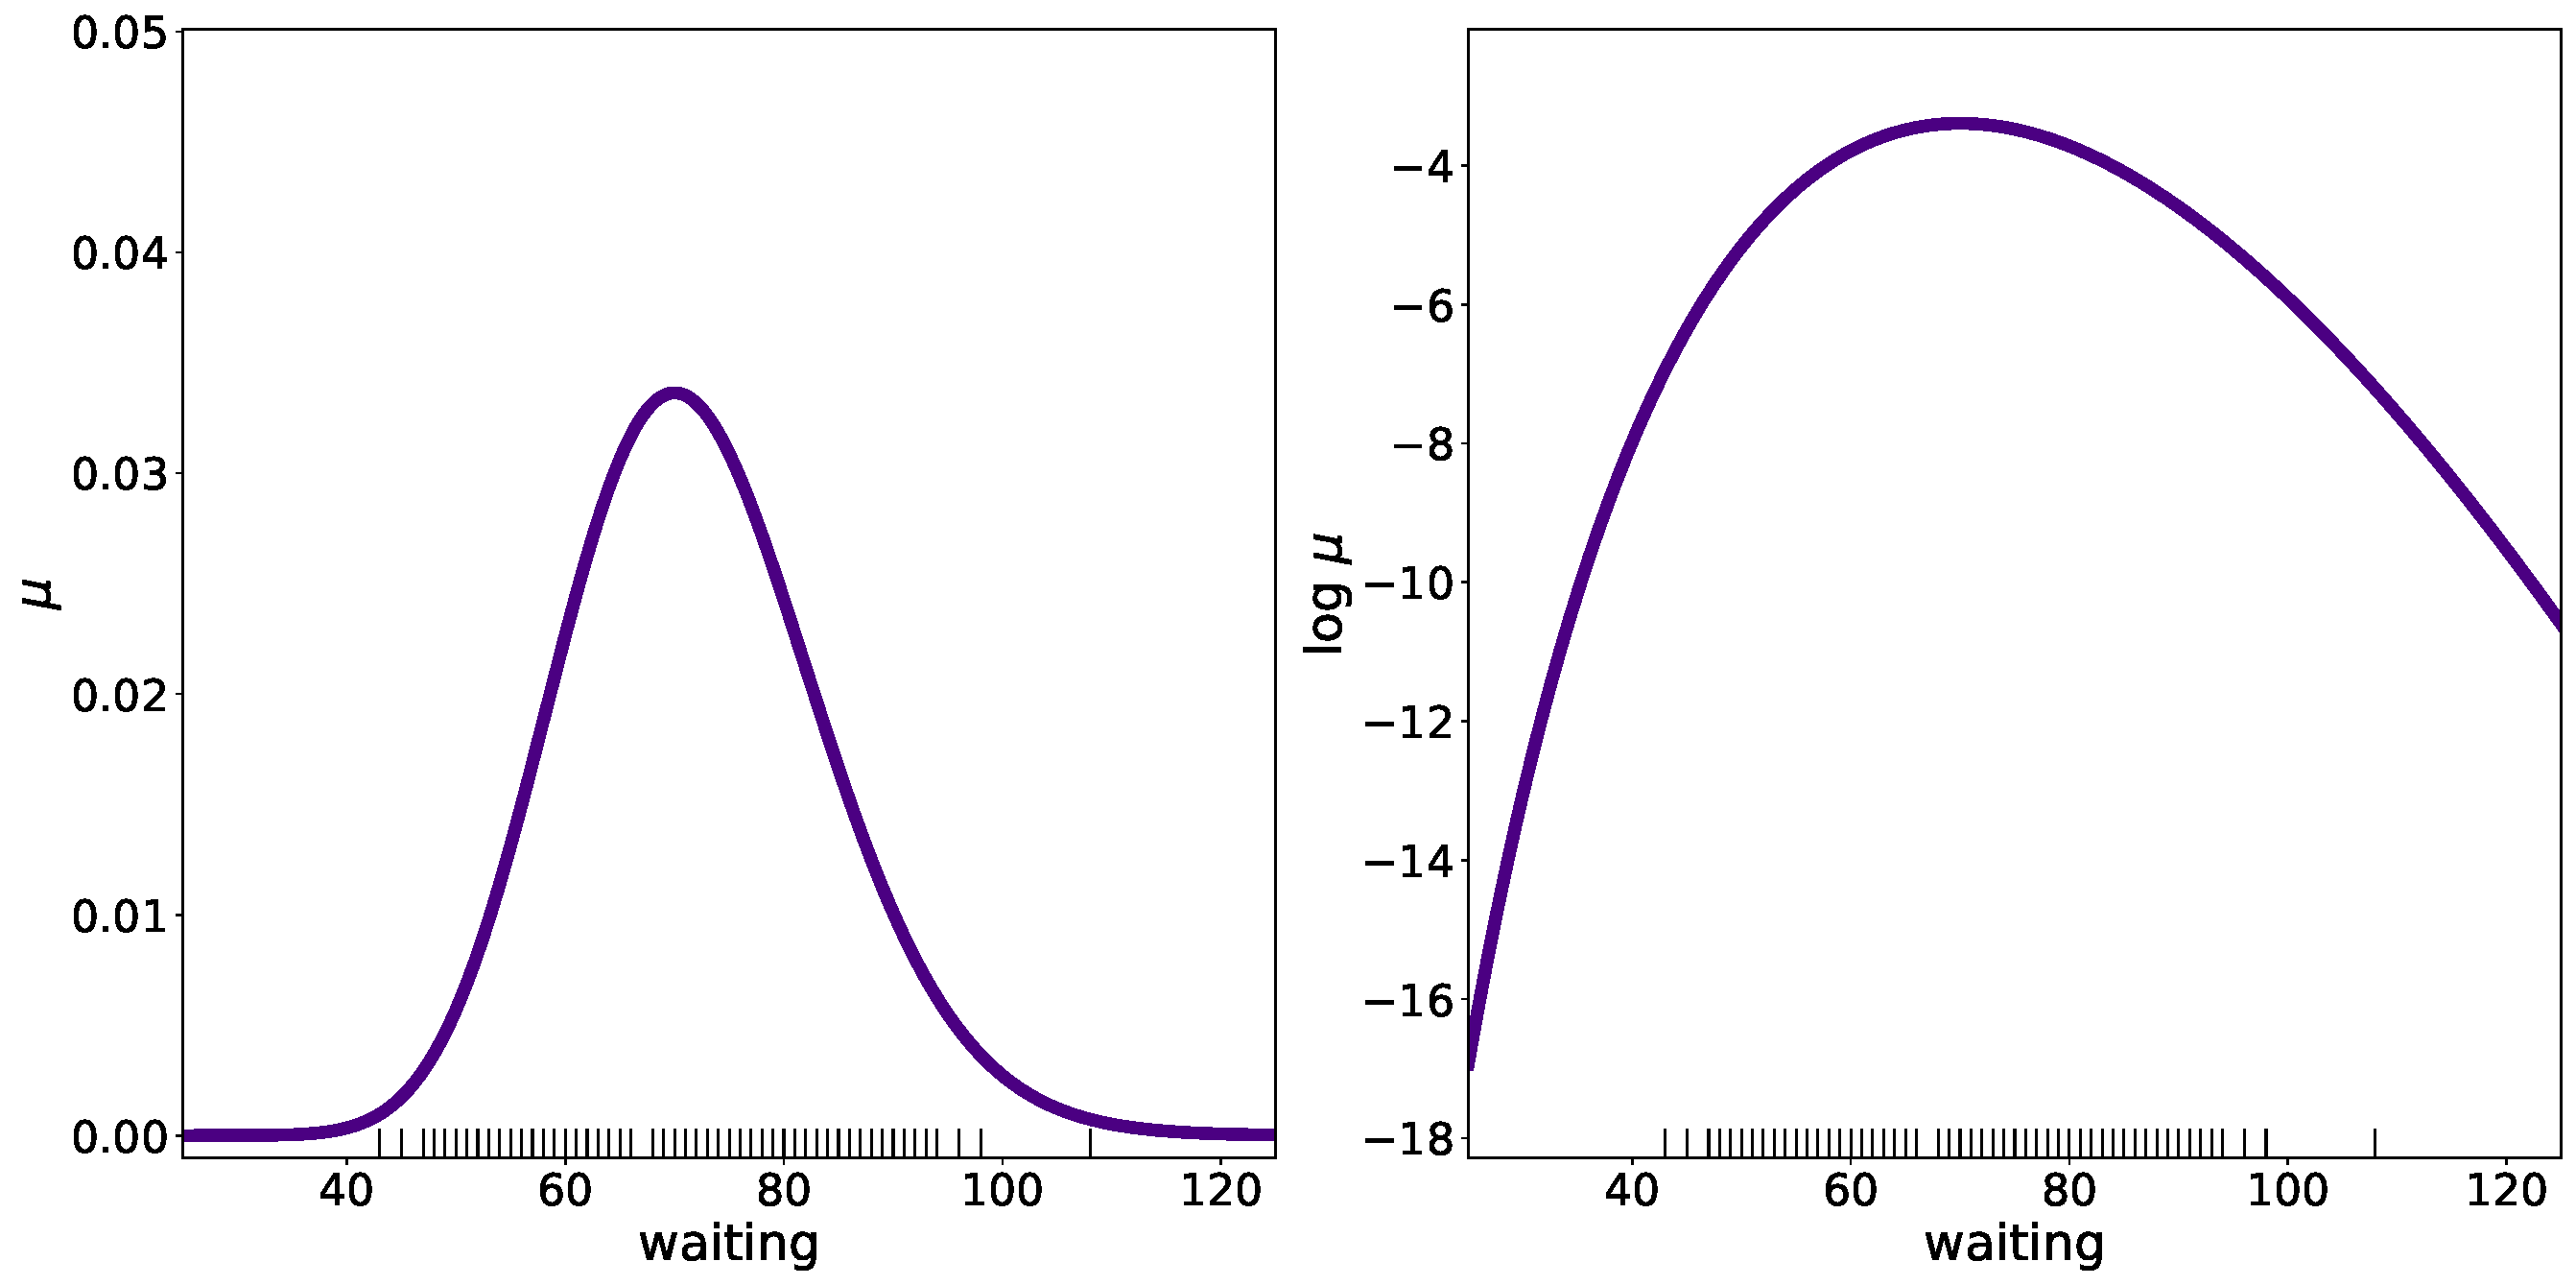
\includegraphics[width=\textwidth]{../plots/baseden-logbaseden-Gamma-36.0-2.0.pdf}
	\caption{Left panel shows $\mu$ and right panel shows $\log \mu$. The rug plot indicates the location of data.}
	\label{fig-base-den-log}
\end{figure}

The resulting early stopping SM density estimates are shown in Figure \ref{fig-early-stopping-estimate}. Note that when the number of iterations $t$ is small, the resulting density estimates are very close to $\mu$, as we expect. As $t$ increases, the density estimates become reasonable and show the bimodal feature of the data. However, as $t$ becomes very large, the density estimates contain a bump or become a spike at the isolated observation 108. We will return to this phenomenon in Section \ref{subsec-smes-limiting-t} and in the subsequent chapters of this dissertation. 

\begin{figure}[t]
	\centering
	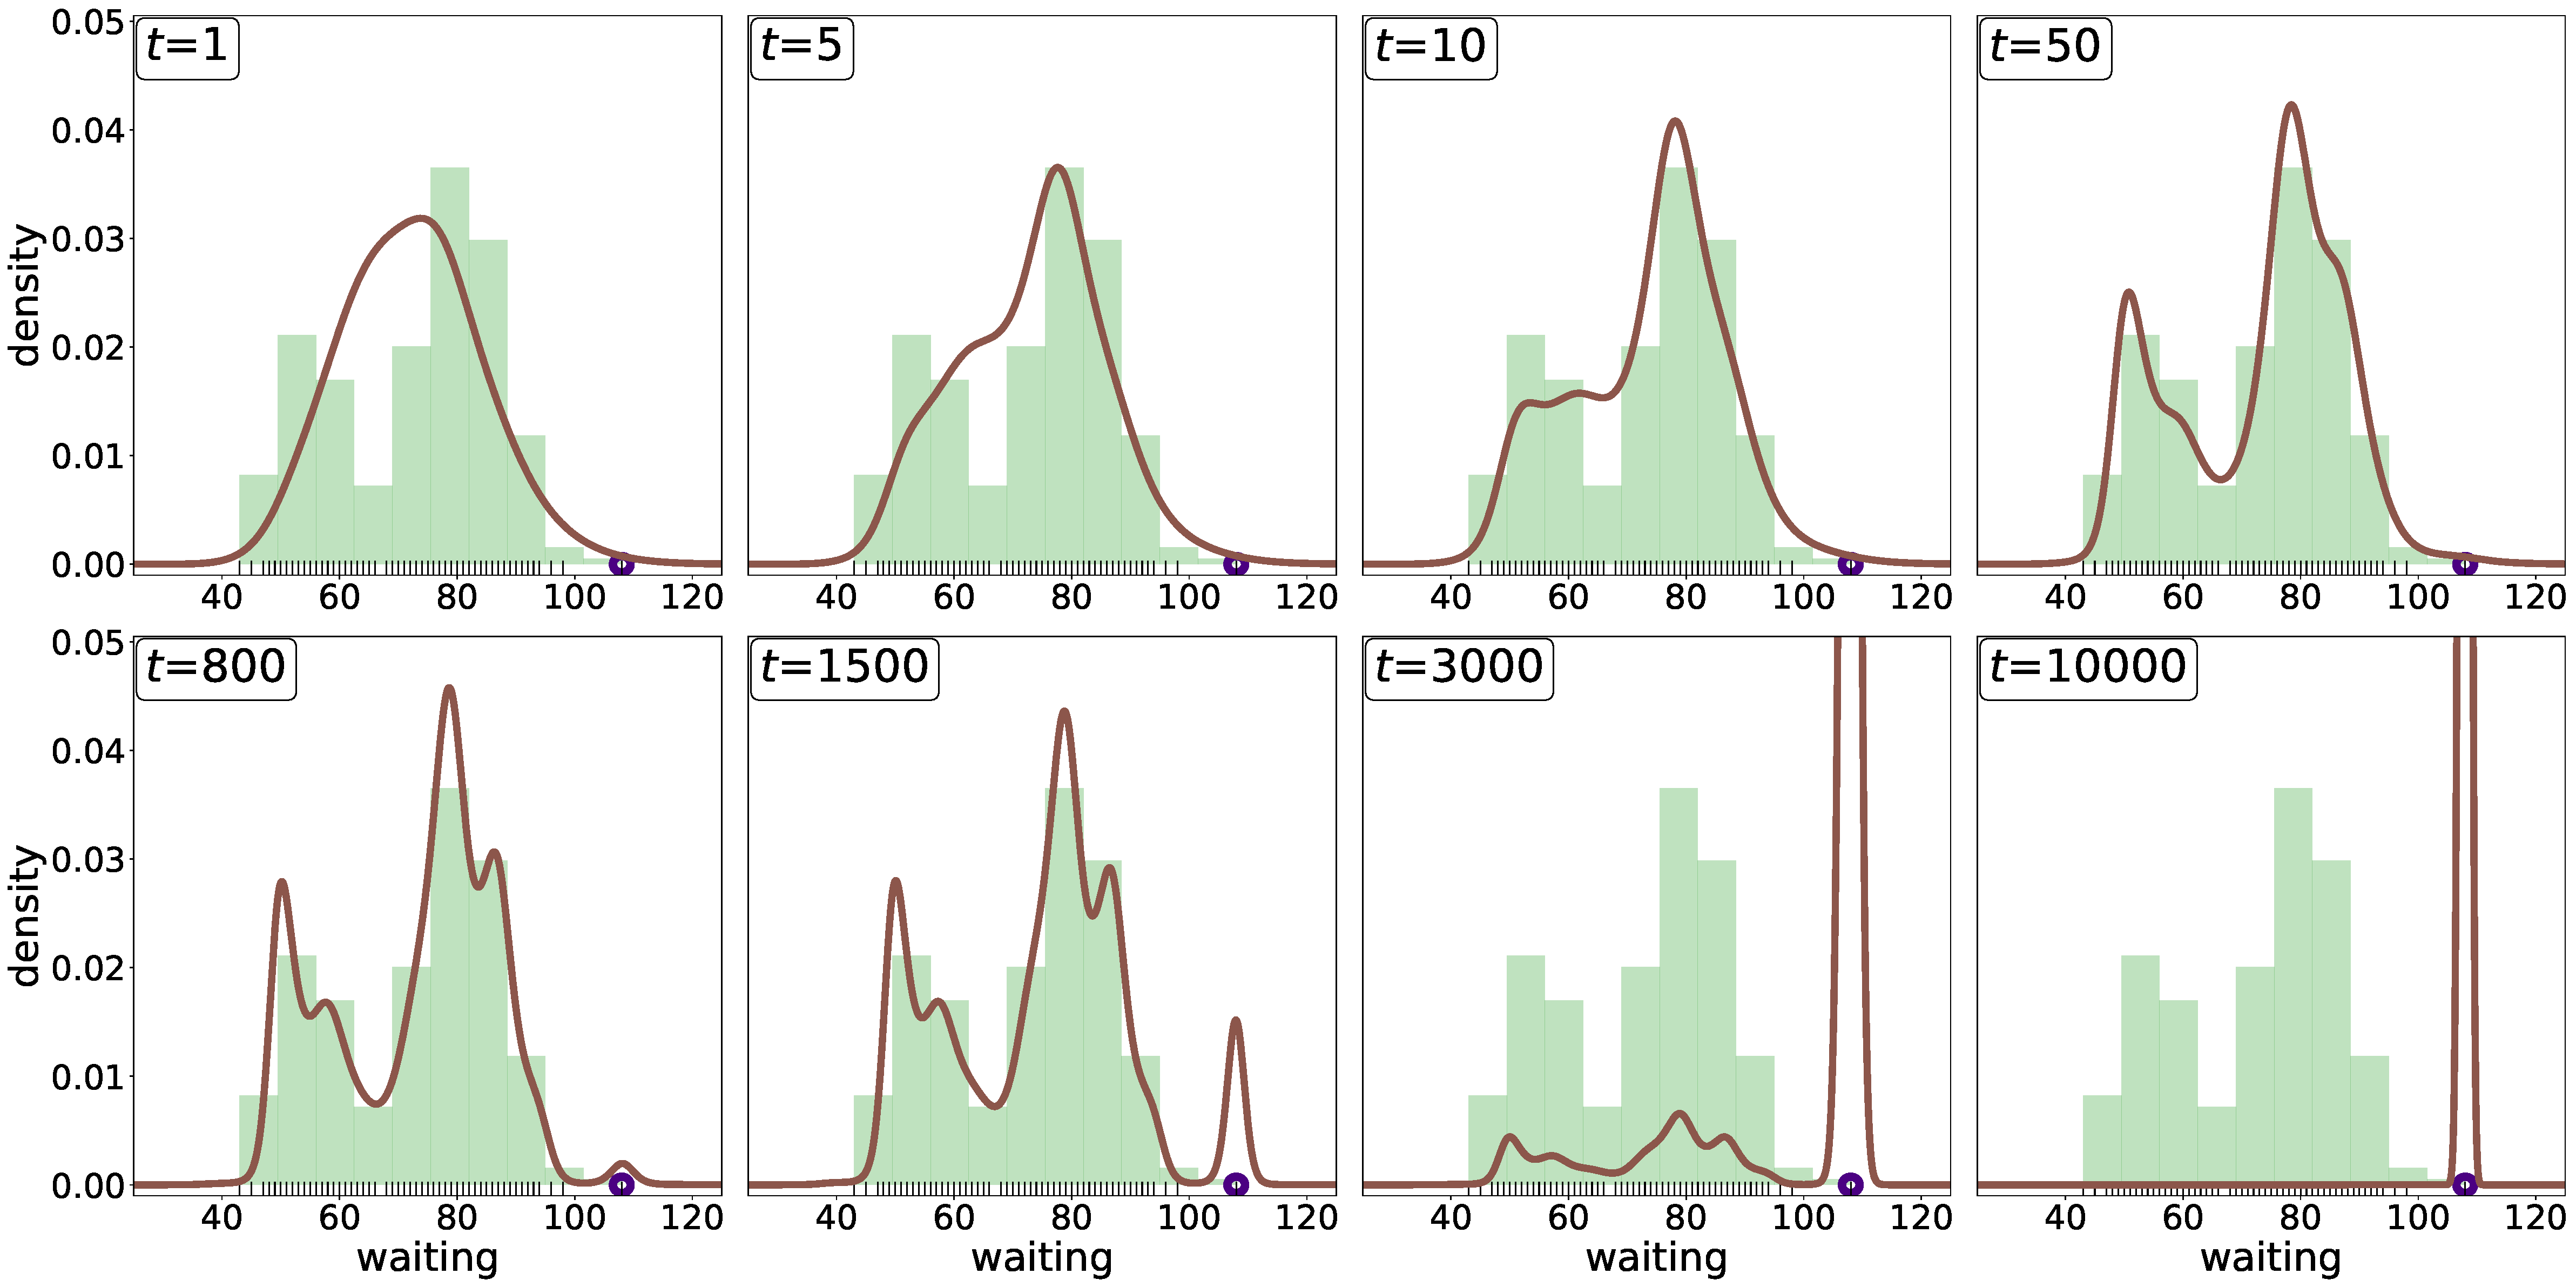
\includegraphics[width=\textwidth]{../plots/waiting-SM-density-estimates-earlystopping-only-bw=5.0-baseden=Gamma-36.0-2.0-entireRKHS.pdf}
	\caption{Early stopping SM density estimates for different values of number of iterations labeled at the upper left corner. Histogram of data with the bin width chosen by the Freedman-Diaconis rule is shown in green. The rug plot indicates the location of data and the purple circle indicates the location of the observation 108.}
	\label{fig-early-stopping-estimate}
\end{figure}

\subsection{When to Terminate the Algorithm}

With the numerical examples shown in the preceding section, we see the choice of the number of iterations is critical to producing satisfactory density estimates. The goal of this section is to discuss how to determine when to terminate the gradient descent algorithm in practice. We will provide two methods: the hold-out method and the $K$-fold cross validation. 

% We re-emphasize that the number of iterations $t$ in the early stopping approach performs the regularization purpose. If we stop too early, 

The hold-out method randomly partition the entire data into two parts, where one part, denoted by $\bS_{\mathrm{train}}$, 
%:= \sets{X_{\sigma \parens{1}}, \cdots, X_{\sigma \parens{m}}}$, 
is used to perform the gradient descent algorithm and the other part, denoted by $\bS_{\mathrm{test}}$, 
%:= \sets{X_{\sigma \parens{m+1}}, \cdots, X_{\sigma \parens{n}}}$
is used to evaluate the performance of the corresponding gradient descent iterate. 
%, where $\sigma \parens{i}$ denotes the index of data after the random shuffling for all $i = 1, \cdots, n$. 
%Let 
%\begin{align*}
%	\widehat{J}_{\SM, \mathrm{train}} \parens{f} := \frac{1}{2} \innerp{f}{\widehat{C}_{\mathrm{train}} f}_{\calH} - \innerp{f}{\hat{z}_{\mathrm{train}}}_{\calH}, \qquad \widehat{J}_{\SM, \mathrm{test}} \parens{f} := \frac{1}{2} \innerp{f}{\widehat{C}_{\mathrm{test}} f}_{\calH} - \innerp{f}{\hat{z}_{\mathrm{test}}}_{\calH}
%\end{align*}
%where 
%\begin{align*}
%	\widehat{C}_{\mathrm{train}} := \frac{1}{m} \sum_{i=1}^m \sum_{u=1}^d \partial_u k \parens{X_{\sigma \parens{i}}, \,\cdot\,} \otimes \partial_u k \parens{X_{\sigma \parens{i}}, \,\cdot\,}
%\end{align*}
Let $\widehat{J}_{\SM, \mathrm{train}}$ and $\widehat{J}_{\SM, \mathrm{test}}$ be the SM loss functionals constructed using data in $\bS_{\mathrm{train}}$ and data in $\bS_{\mathrm{test}}$, respectively. Starting from $\hat{f}^{\parens{0}} = 0$, we perform the gradient descent algorithm on $\widehat{J}_{\SM, \mathrm{train}}$, and after obtaining a gradient descent iterate $\hat{f}^{\parens{t}}$, we compute $\widehat{J}_{\SM, \mathrm{test}} \parens{\hat{f}^{\parens{t}}}$, and terminate when $\widehat{J}_{\SM, \mathrm{test}} \parens{\hat{f}^{\parens{t+1}}} > \widehat{J}_{\SM, \mathrm{test}} \parens{\hat{f}^{\parens{t}}}$. The algorithm is shown in Algorithm \ref{algo-early-stopping-holdout}. 

\begin{algorithm}
\caption{Hold-out method to determine when to terminate}\label{algo-early-stopping-holdout}
\begin{algorithmic}[1]
\Statex \algorithmicrequire 
\begin{itemize}\setlength\itemsep{0em}
	\item $X_1, \cdots, X_n$, the data from $p_0$; 
	\item $m < n$, the number of observations in $\bS_{\mathrm{train}}$; 
	\item $\tau$, the constant step size. 
\end{itemize}

\State Randomly shuffle the data $X_1, \cdots, X_n$, and let the first $m$ observations be $\bS_{\mathrm{train}}$ and the remaining be $\bS_{\mathrm{test}}$; 
\State Let \texttt{error1} = $\widehat{J}_{\SM, \mathrm{test}} \parens{\hat{f}^{\mathtt{old}}}$, where $\hat{f}^{\mathtt{old}} = \hat{f}^{\parens{0}} = 0$; 
\State Let $\hat{f}^{\mathtt{new}} = \hat{f}^{\mathtt{old}} - \tau \nabla \widehat{J}_{\SM, \mathrm{train}} \parens{\hat{f}^{\mathtt{old}}}$; 
\State Compute \texttt{error2} = $\widehat{J}_{\SM, \mathrm{test}} \parens{\hat{f}^{\mathtt{new}}}$; 
\While{\texttt{error1} $>$ \texttt{error2}}
\State Let $\hat{f}^{\mathtt{old}} = \hat{f}^{\mathtt{new}}$ and \texttt{error1} = \texttt{error2};  
\State Update $\hat{f}^{\mathtt{new}} = \hat{f}^{\mathtt{old}} - \tau \nabla \widehat{J}_{\SM, \mathrm{train}} \parens{\hat{f}^{\mathtt{old}}}$; 
\State Compute \texttt{error2} = $\widehat{J}_{\SM, \mathrm{test}} \parens{\hat{f}^{\mathtt{new}}}$; 
\EndWhile
\State \Return $\hat{f}^{\mathtt{old}}$. 
\end{algorithmic}
\end{algorithm}

The major drawback of this hold-out method is that it has to set aside a portion of data for the evaluation purpose, rather than use the entire data for the estimation purpose. 

The second method is the $K$-fold cross-validation (CV). We first specify a set of number of iterations candidates to terminate the algorithm, and randomly partition all data into $K$ folds of (roughly) equal size. Let us fix one number of iterations candidate, say $t_0$, for now. We use $K-1$ folds of data to perform the gradient descent algorithm and terminate at $t_0$, and evaluate the SM loss functional constructed using data in the remaining fold at this gradient descent iterate. Note that, for this particular $t_0$, we end up with $K$ values of the SM loss functional, one obtained from each fold. We average all these $K$ values and regard this average as the estimated risk of $t_0$. Repeat this process for each number of iterations candidate, and obtain an estimated risk from each of them. The best number of iterations is the one with the lowest estimated risk. In the end, we perform the gradient descent algorithm on the entire data and terminate at this best number of iterations. It is obvious that the final early stopping SM density estimate utilizes all data and avoid the drawback in the hold-out method. The complete algorithm of this $K$-fold CV method is shown in Algorithm \ref{algo-early-stopping-cv}. 

\begin{algorithm}
\caption{$K$-fold cross-validation method to determine when to terminate}\label{algo-early-stopping-cv}
\begin{algorithmic}[1]
\Statex \algorithmicrequire 
\begin{itemize}\setlength\itemsep{0em}
	\item $X_1, \cdots, X_n$, the data from $p_0$; 
	\item $K$, the number of folds for cross validation; 
	\item $\tau$, the constant step size; 
	\item $t_1, \cdots, t_m$, a list of number of iterations candidates to terminate. 
\end{itemize}

\State Randomly partition the data $X_1, \cdots, X_n$ into $K$ folds of (roughly) equal size, denoted by $\bS_{1}, \cdots, \bS_{K}$; 
\State Set \texttt{metric} to be an empty list to record the estimated risks for different number of iterations candidates; 
\For{$j = 1, \cdots, m$}
\State Set \texttt{metric\_j} = 0; 
\For{$\ell = 1, \cdots, K$}
\State Let $\bS_{\mathrm{test}} = \bS_{\ell}$ and $\bS_{\mathrm{train}}$ contain data excluding $\bS_{\ell}$; 
\State Perform the gradient descent algorithm on $\widehat{J}_{\SM, \mathrm{train}}$, which is the SM loss functional constructed using data in $\bS_{\mathrm{train}}$, and terminate at $t_j$; denote the resulting natural parameter by $\hat{f}_{\ell}^{\parens{t_j}}$; 
\State Update \texttt{metric\_j} += $\widehat{J}_{\SM, \mathrm{test}} \parens{\hat{f}_{\ell}^{\parens{t_j}}}$, where $\widehat{J}_{\SM, \mathrm{test}}$ is the SM loss functional constructed using data in $\bS_{\mathrm{test}}$; 
\EndFor
\State Append \texttt{metric\_j}/$K$ to the end of \texttt{metric}; 
\EndFor
\State Let $m^* \in \sets{1, \cdots, m}$ be the one with the lowest value in \texttt{metric}. Then, $t_{m^*}$ is the best number of iterations; 
\State Perform the gradient descent algorithm on $\widehat{J}_{\SM}$, the SM loss functional constructed using \emph{all} data, and terminate at $t_{m^*}$. 
\State \Return $\hat{f}^{\parens{t_{m^*}}}$. 
\end{algorithmic}
\end{algorithm}


\section{Theoretical Properties}\label{section-theoretical-properties}

With the introduction to our early stopping SM density estimator and its computation, we discuss its theoretical properties in this section. 

We will assess its theoretical properties from two aspects. First, we will look at what happens to the density estimator if we do not terminate the gradient descent algorithm and let the number of iterations approach to $\infty$. This will be covered in Section \ref{subsec-smes-limiting-t}. 

Second, in this early stopping approach, we use the number of iterations as a tuning parameter to perform implicit regularization, which plays exactly the same role as the penalty parameter $\rho$ in the penalized approach. We derive a (theoretical) stopping rule and establish the convergence rates of the resulting natural parameter estimator and the density estimator using this stopping rule in Section \ref{subsec-nonasymp-t}.

\subsection{Density Estimator Without Termination} \label{subsec-smes-limiting-t}

In this section, we investigate the behavior of the early stopping SM density estimator if we keep running the gradient descent algorithm without termination. 

Our main theorem is the following. 

\begin{theorem}\label{thm-limiting-density-t}
	Let $\hat{z}_2 \in \calH$ be the orthogonal projection of $\hat{z}$ onto $\range \parens{\widehat{C}}^{\perp}$, the orthogonal complement of $\range \parens{\widehat{C}}$. In addition to \ref{assumption-2-1-inf-dim} - \ref{assumption-2-4-base-density} in Chapter \ref{ch2} and \ref{assumption-1} - \ref{assumption-5}, we further assume 
	\begin{enumerate}[label=\textbf{(C\arabic*)}]
		\item \label{assumption-limiting-1} there exists a unique $x^* \in \calX$ such that 
		%$\hat{z}_2 \parens{x^*} \ge \hat{z}_1 \parens{x}$ for all $x \in \calX$ and 
		$\hat{z}_2 \parens{x^*} > \hat{z}_2 \parens{x}$ for all $x \in \calX \backslash \sets{x^*}$, and 
		\item \label{assumption-limiting-2} $\tau \in \parens{0, 1 / \parens{d \kappa_2^2}}$. 
	\end{enumerate}
	Then, $\lim_{t \to \infty} q_{\hat{f}^{\parens{t}}} \parens{x^*} = \infty$. 
\end{theorem}

\begin{remark}
	We can relax \ref{assumption-limiting-1} to the one that the maximizers of $\hat{z}_2$ form a set of Lebesgue measure zero. Let $\calM$ denote the set of all maximizers of $\hat{z}_2$. Then, we can modify the proof slightly and conclude $\lim_{t \to \infty} q_{\hat{f}^{\parens{t}}} \parens{x^*} = \infty$ at all $x^* \in \calM$. 
\end{remark}

The proof of Theorem \ref{thm-limiting-density-t} will be provided in Section \ref{subsection-proof-smes-limiting-t}, and is built upon the decomposition of $\hat{f}^{\parens{t}}$ which we now look at. 

\subsubsection{Decomposition of Gradient Descent Iterates}

We decompose $\hat{f}^{\parens{t}}$ into two parts, where one part resides in $\range \parens{\widehat{C}}$ and the other resides in $\range \parens{\widehat{C}}^{\perp}$, the orthogonal complement of $\range \parens{\widehat{C}}$. 

As we have discussed in Section \ref{subsection-first-algorithm}, $\range \parens{\widehat{C}}$ contains all functions that can be written as a linear combination of $\partial_u k \parens{X_i, \,\cdot\,}$, for all $i = 1, \cdots, n$ and $u = 1, \cdots, d$, which is of finite dimension and forms a closed linear subspace of $\calH$ \parencite[Corollary 6 in Section 13.3 in][]{Royden2018-cd}. Its orthogonal complement is 
\begin{align*}
	\range \parens{\widehat{C}}^{\perp} := \sets[\Big]{g \in \calH \Bigm| \innerp{g}{f}_{\calH} = 0, \text{ for all } f \in \range \parens{\widehat{C}}}, 
\end{align*}
which also forms a closed linear subspace of $\calH$ \parencite[Section 16.1 in][]{Royden2018-cd}.  

Notice that $\range \parens{\widehat{C}}^{\perp} \neq \sets{0}$. To see this, suppose the opposite. Then, we have $\range \parens{\widehat{C}} = \calH$ \parencite[Corollary 4 in Section 16.1 in][]{Royden2018-cd}. But, since $\range \parens{\widehat{C}}$ is finite-dimensional, $\range \parens{\widehat{C}} = \calH$ implies $\calH$ is also finite-dimensional. This contradicts to \ref{assumption-2-1-inf-dim} in Chapter \ref{ch2} that $\calH$ is infinite-dimensional. 

Now, decompose $\hat{z}$ into two parts, $\hat{z}_1$ and $\hat{z}_2$, where $\hat{z}_1 := \Pi_{\range \parens{\widehat{C}}} \parens{\hat{z}} \in \range \parens{\widehat{C}}$, $\hat{z}_2 := \Pi_{\range \parens{\widehat{C}}^{\perp}} \parens{\hat{z}} \in \range \parens{\widehat{C}}^{\perp}$, and $\Pi_S \parens{\hat{z}}$ denotes the orthogonal projection of $\hat{z}$ onto the closed linear subspace $S$ of $\calH$. Note that both $\hat{z}_1$ and $\hat{z}_2$ are well-defined by the projection theorem in a Hilbert space \parencite[Theorem 2.3.1 in][]{Brockwell2013-dq}. 

Recall that $\hat{z} = - \frac{1}{n} \sum_{i=1}^n \sum_{u=1}^d \parens[\big]{\parens{\partial_u \log \mu} \parens{X_i} \partial_u k \parens{X_i, \,\cdot\,} + \partial_u^2 k \parens{X_i, \,\cdot\,}}$ involves the first two partial derivatives of $k$. The component $- \frac{1}{n} \sum_{i=1}^n \sum_{u=1}^d \partial_u \log \mu \parens{X_i} \partial_u k \parens{X_i, \,\cdot\,}$ must belong to $\range \parens{\widehat{C}}$, and the component $- \frac{1}{n} \sum_{i=1}^n \sum_{u=1}^d \partial_u^2 k \parens{X_i, \,\cdot\,}$ does \emph{not} necessarily belong to $\range \parens{\widehat{C}}$, except for special choices of $k$. We assume $\hat{z}_2 \neq 0$ for the rest of this section. 

In addition, since $\hat{z}_1 \in \range \parens{\widehat{C}}$, we can find $\hat{g}_1 \in \range \parens{\widehat{C}}$ satisfying $\hat{z}_1 = \widehat{C} \hat{g}_1$. We claim such a choice of $\hat{g}_1$ is unique. Suppose there exists $\tilde{g}_1 \in \range \parens{\widehat{C}}$ and $\tilde{g}_1 \neq \hat{g}_1$ such that $\hat{z}_1 = \widehat{C} \tilde{g}_1$, then $0 = \widehat{C} \parens{\hat{g}_1 - \tilde{g}_1}$, implying that $\hat{g}_1 - \tilde{g}_1 = 0$ or $\hat{g}_1 - \tilde{g}_1 \in \range \parens{\widehat{C}}^{\perp}$ is nonzero. Since $\range \parens{\widehat{C}}$ is a closed linear subspace of $\calH$, the latter case cannot happen. We deduce that $\tilde{g}_1 = \hat{g}_1$, and the uniqueness follows. 

With the decomposition of $\hat{z}$ we have discussed so far, the following proposition decomposes $\hat{f}^{\parens{t}}$ into two components. %, where one component belongs to $\range \parens{\widehat{C}}$ and the other belongs to $\range \parens{\widehat{C}}^{\perp}$. 

\begin{proposition}\label{prop-decomposition-ft}
	Suppose $\hat{f}^{\parens{0}} = 0 \in \calH$. The $\parens{t+1}$-st gradient descent iterate $\hat{f}^{\parens{t+1}}$, for each $t \in \Natural_0$, can be written as the sum of the following two components 
	\begin{align*}
		\hat{f}_1^{\parens{t+1}} := & \,  \parens{I - \parens{I - \tau \widehat{C}}^{t+1}} \hat{g}_1 \in \range \parens{\widehat{C}}\\ 
		\hat{f}_2^{\parens{t+1}} := & \, \parens{t+1} \tau \hat{z}_2 \in \range \parens{\widehat{C}}^{\perp}
	\end{align*}
\end{proposition}

The following proposition gives explicit formulae for $\hat{z}_1$, $\hat{z}_2$, and $\hat{g}_1$. 

\begin{proposition}\label{prop-hatz1-hatz2-g1}
	Let $\bG \in \Real^{nd \times nd}$ and $\bh \in \Real^{nd}$ be the quantities defined in Theorem \ref{thm-early-stopping-algo} and assume $\bG$ is positive definite. Then, 
	\begin{enumerate}[label=(\alph*)]
		\item \label{prop-hatz1-hatz2-g1-1} $\hat{z}_1 = \sum_{i=1}^n \sum_{u=1}^d \alpha^*_{\parens{i-1}d+u} \partial_u k \parens{X_i, \,\cdot\,}$, where $\balpha^* := \parens{\alpha^*_{1}, \cdots, \alpha^*_{nd}} \in \Real^{nd}$ satisfies the linear system $\bG \balpha^* = \bh$; 
		\item \label{prop-hatz1-hatz2-g1-2} $\hat{z}_2 = \sum_{i=1}^n \sum_{u=1}^d \bracks[\big]{ \parens[\big]{- \frac{1}{n} \parens{\partial_u \log \mu} \parens{X_i} - \alpha^*_{\parens{i-1}d+u}} \partial_u k \parens{X_i, \,\cdot\,} - \frac{1}{n} \partial_u^2 k \parens{X_i, \,\cdot\,}}$; 
		\item \label{prop-hatz1-hatz2-g1-3} $\hat{g}_1 = \sum_{i=1}^n \sum_{u=1}^d \beta^*_{\parens{i-1}d+u} \partial_u k \parens{X_i, \,\cdot\,}$, where $\bbeta^* := \parens{\beta_1^*, \cdots, \beta_{nd}^*} \in \Real^{nd}$ satisfies the linear system $\frac{1}{n} \bG \bbeta^* = \balpha^*$. 
	\end{enumerate}
\end{proposition}

Now that we have decomposed $\hat{f}^{\parens{t+1}}$ into two components, the following proposition established the boundedness of $\hat{f}_1^{\parens{t+1}}$ over $\calX$ for all $t \in \Natural_0$. 

\begin{proposition}\label{proposition-bound-hatz1}
	Under the same assumptions in Theorem \ref{thm-limiting-density-t}, there exists $M > 0$ such that, for all $x \in \calX$ and all $t \in \Natural_0$, $\abs{\innerp{\hat{f}_1^{\parens{t+1}}}{k \parens{x, \,\cdot\,}}_{\calH}} \le M$. 
\end{proposition}

The proofs of Propositions \ref{prop-decomposition-ft} - \ref{proposition-bound-hatz1} can be found in Section \ref{subsection-proof-smes-limiting-t}. 

Even though $\hat{f}_1^{\parens{t+1}}$ is bounded over $\calX$ for all $t \in \Natural_0$, $\hat{f}_2^{\parens{t+1}}$ is \emph{not}. In particular, since $\hat{f}_2^{\parens{t+1}} = \parens{t+1} \tau \hat{z}_2$, we have 
\begin{align*}
	\abs{ \innerp{\hat{f}_2^{\parens{t+1}}}{ k \parens{x, \,\cdot\,}}_{\calH} } = \parens{t+1} \tau \abs{\innerp{\hat{z}_2}{k \parens{x, \,\cdot\,}}_{\calH} } \to \infty, \qquad \text{ as } t \to \infty, 
\end{align*}
unless $\innerp{\hat{z}_2}{k \parens{x, \,\cdot\,}}_{\calH} = 0$. 


\subsubsection{Numerical Illustration of Theorem \ref{thm-limiting-density-t}}

We use the \texttt{waiting} variable in the Old Faithful Geyser dataset to illustrate Theorem \ref{thm-limiting-density-t}. 

With the help of \eqref{eq-hatz} in Chapter \ref{ch2} and Proposition \ref{prop-hatz1-hatz2-g1}, we plot $\hat{z}$, $\hat{z}_1$ and $\hat{z}_2$ in Figure \ref{fig-decomposition-hatz}. In particular, note that, from the right panel of Figure \ref{fig-decomposition-hatz}, $\hat{z}_2$ achieves the maximum at $108$. With Theorem \ref{thm-limiting-density-t}, we expect see that, as the number of iterations $t$ keeps increasing, the density value at $108$ also keeps increasing. Figure \ref{fig-density-val-108-vs-t}, the plot of the density value at 108 against the number of iterations, coincides with our expectation. 

\begin{figure}[t]
	\centering
	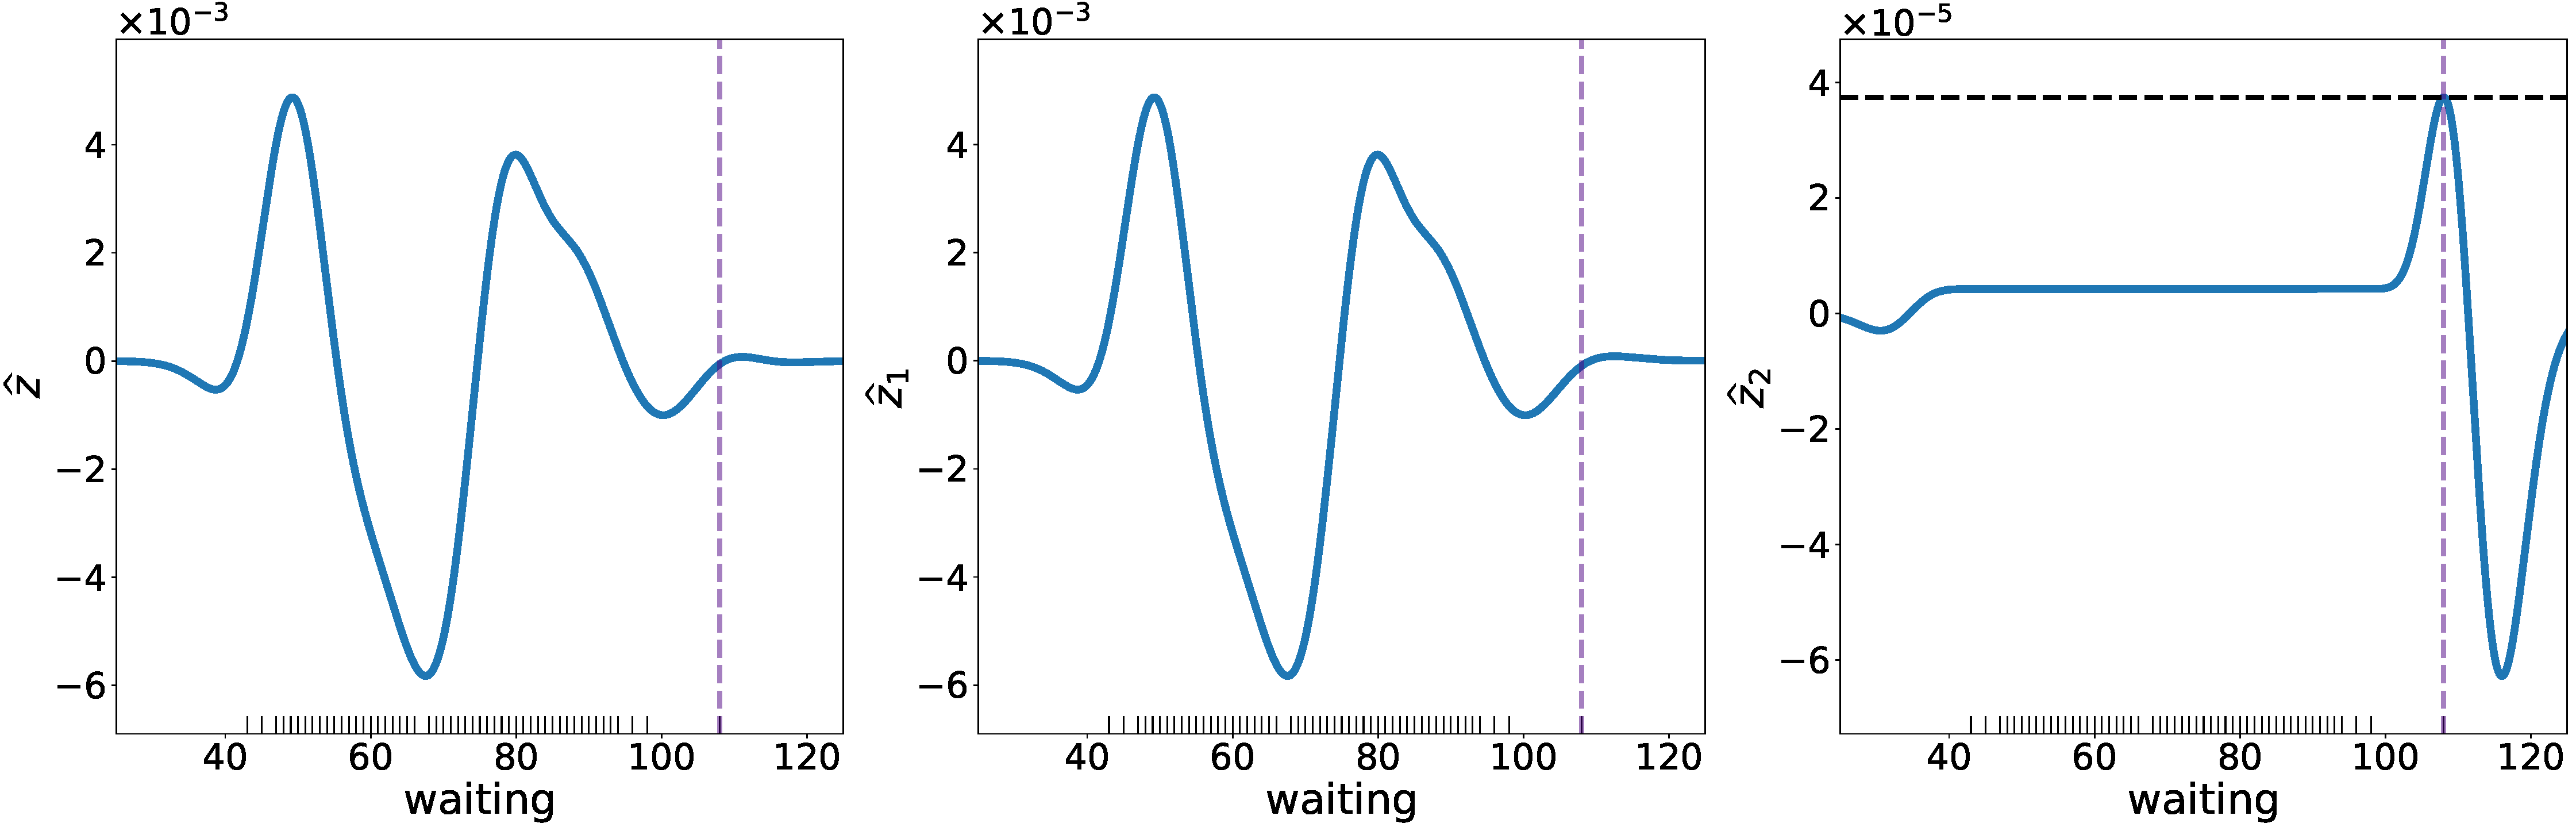
\includegraphics[width=\textwidth]{../plots/decomposition-hat-z-bw=5.0-Gamma-36.0-2.0.pdf}
	\caption{Plots of $\hat{z}$ (left panel), $\hat{z}_1$ (middle panel) and $\hat{z}_2$ (right panel). The rug plot indicates the location of data.}
	\label{fig-decomposition-hatz}
\end{figure}

\begin{figure}[h]
	\centering
	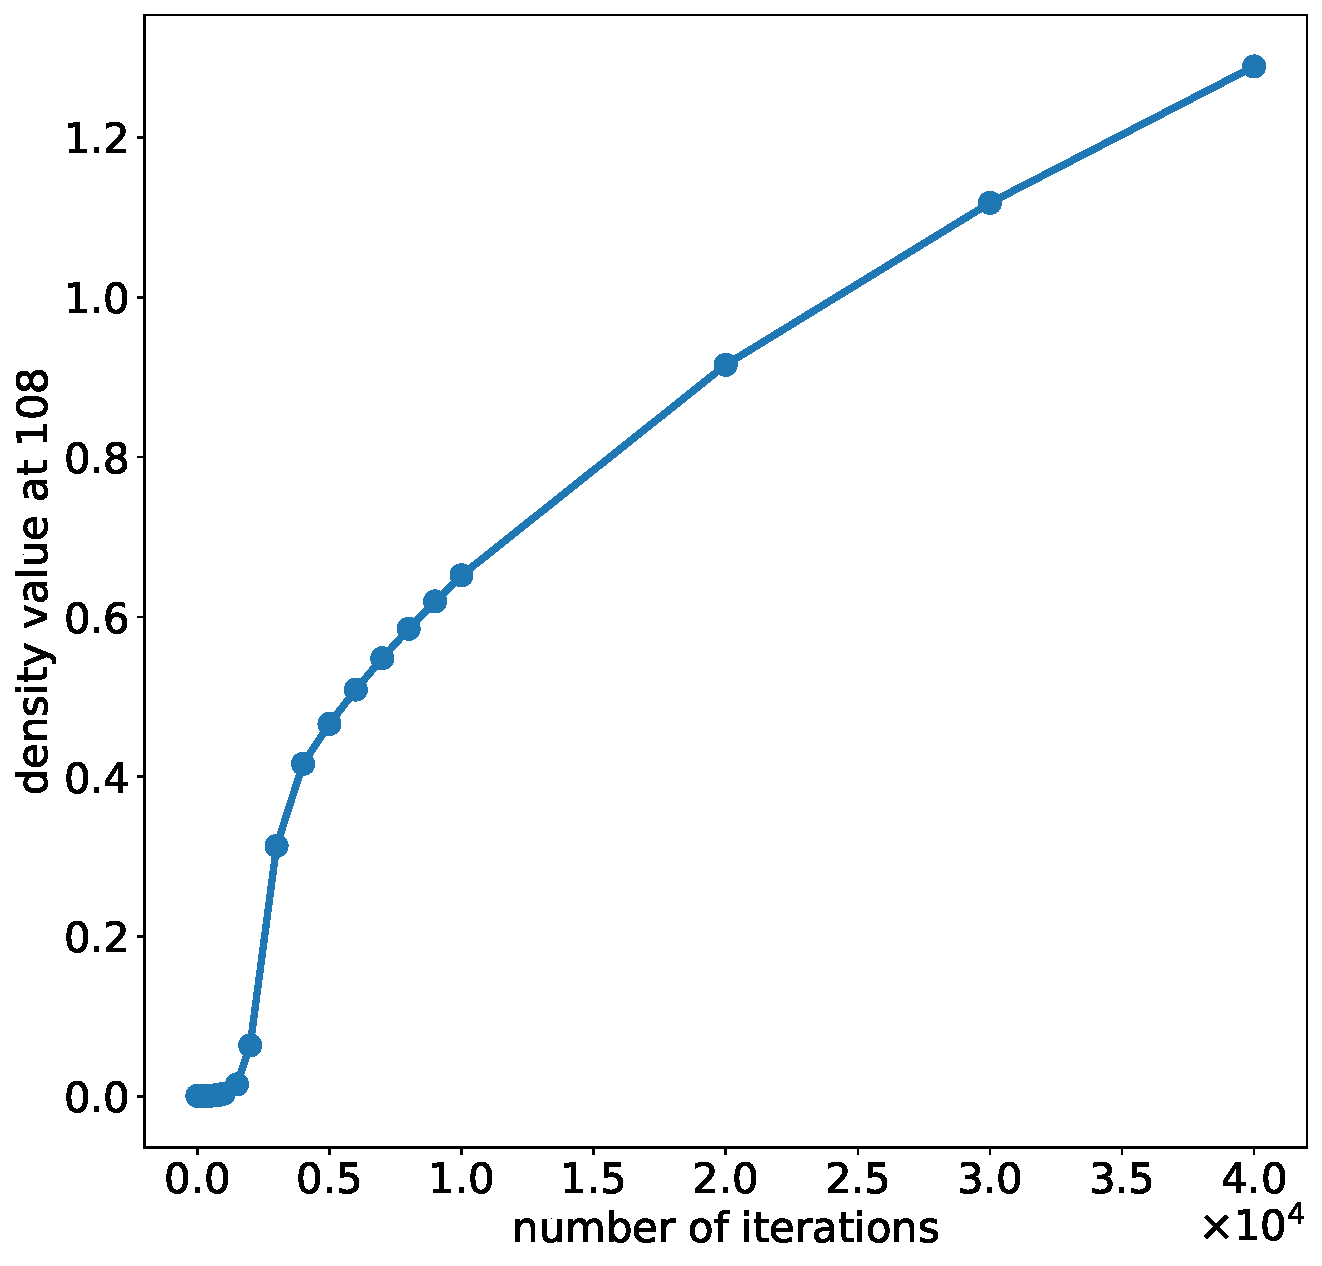
\includegraphics[width=0.6\textwidth]{../plots/density-at-108-vs-number-iterations-Gamma-36.0-2.0.pdf}
	\caption{Density value at $108$ against the number of iterations.}
	\label{fig-density-val-108-vs-t}
\end{figure}

\subsection{Rate of Convergence} \label{subsec-nonasymp-t}

We study the rate of convergence of the early stopping SM density estimator in this section. More specifically, we attempt to answer the following questions: 
\begin{enumerate}
	% \item What is the (theoretically) optimal number of iterations? In what sense is this number of iterations optimal? 
	\item Suppose $p_0 = q_{f_0} \in \calQ_{\ker}$ for some $f_0 \in \calH$. What can we say about the gap between $\hat{f}^{\parens{t}}$ and $f_0$, for each $t \in \Natural$? 
	\item What can we say about the gap between $q_{\hat{f}^{\parens{t}}}$ and $p_0$, for each $t \in \Natural$? 
	\item Based on the gaps above, can we derive an early stopping rule? 
\end{enumerate}

Throughout this section, besides \ref{assumption-1} - \ref{assumption-5}, we further assume the following: 
\begin{enumerate}[label=\textbf{(B\arabic*)}, resume=assumptions]
	\item \label{assumption-6} The true density $p_0$ belongs to $\calQ_{\ker}$ and there exists $f_0 \in \calH$ such that $p_0 = q_{f_0}$. % https://tex.stackexchange.com/questions/455028/continuing-the-enumerate-numbering-from-other-the-enumerate-list-in-the-document, continue the numbering from the previous enumeration 
	\item \label{assumption-7} There exists $\gamma > 0$ such that $f_0 \in \range \parens{C^\gamma}$, where $C: \calH \to \calH$ is given by \eqref{eq-C-def}. That is, there exists $g_0 \in \calH$ such that $C^{\gamma} g_0 = f_0$. 
\end{enumerate}

Our main result is the following theorem. 

\begin{theorem}\label{theorem-convergence-rate}
	Under \ref{assumption-2-1-inf-dim} - \ref{assumption-2-4-base-density} in Chapter \ref{ch2} and \ref{assumption-1} - \ref{assumption-7}, for each $n \in \Natural$, there exists an early stopping rule 
	\begin{align*}
		t^*: \Natural & \, \to \Natural, \qquad \qquad n \mapsto \ceil{n^{\frac{1}{2 \parens{\gamma + 2}}}}
	\end{align*}
	such that, with probability at least $1 - \delta$ for $\delta \in \parens{0, 1}$, the following inequality holds 
	\begin{align*}
		\norm{\hat{f}^{\parens{t^* \parens{n}}} - f_0}_{\calH} \le & \, \parens{4 C_1 + C_2} n^{-\frac{\gamma}{2 \parens{\gamma+2}}}, 
	\end{align*}
	where $C_1 := 2d\tau \parens{\kappa_3 + \kappa_4} \parens{\tau d \kappa_2^2 + 1} \sqrt{2 \log \parens{2 / \delta}}$ and $C_2 := \gamma^{\gamma} \norm{g_0}_{\calH} / \parens{\tau e}^{\gamma}$. 
\end{theorem}

The proof follows \textcite{Yao2007-ji} and details will be provided in Section \ref{proof-theorem-convergence-rate}. The proof depends on the analysis of two sequences of gradient descent iterates: one is the gradient descent iterates derived from the SM loss functional $\widehat{J}_{\SM}$ (which depends on finitely many samples) and the other one is the gradient descent iterates derived from the H-divergence $J_{\SM} \parens{f}$ which can be viewed as the SM loss functional with infinitely many samples, i.e., the population-version SM loss functional. We denote the former sequence by $\sets{\hat{f}^{\parens{t}}}_{t \in \Natural}$ as before and the latter one by $\sets{f^{\parens{t}}}_{t \in \Natural}$, and let both start from the zero function, i.e., $f^{\parens{0}} = \hat{f}^{\parens{0}} = 0 \in \calH$. Using the triangle inequality, we can bound $\norm{\hat{f}^{\parens{t}} - f_0}_{\calH}$ from above by 
\begin{align}\label{eq-sample-plus-approx-errors}
	\norm{\hat{f}^{\parens{t}} - f_0}_{\calH} \le \norm{\hat{f}^{\parens{t}} - f^{\parens{t}}}_{\calH} + \norm{f^{\parens{t}} - f_0}_{\calH}, 
\end{align}
where the population-version sequence of iterates $\sets{f^{\parens{t}}}_{t \in \Natural}$ is used as an intermediary. 

In \eqref{eq-sample-plus-approx-errors}, $\norm{f^{\parens{t}} - f_0}_{\calH}$ is called the \textit{approximation error} (or \textit{bias}), and $\norm{\hat{f}^{\parens{t}} - f^{\parens{t}}}_{\calH}$, is called the \textit{sample error} (or \textit{variance}). We will see later that, as $t$ increases, the derived upper bound of the sample error increases and that of the approximation error decreases. More specifically, as the gradient descent algorithm evolves, the population-version sequence of iterates $\sets{f^{\parens{t}}}_{t \in \Natural}$ converge to $f_0$ eventually but the sample-version sequence of iterates $\sets{\hat{f}^{\parens{t}}}_{t \in \Natural}$ do \emph{not}. Therefore, we have a bias-variance tradeoff we discussed earlier: if we stop the algorithm at a too early time, the resulting $\hat{f}^{\parens{t}}$ has a small variance but a large bias; and, on the other hand, if we keep running it and terminate too late, the resulting $\hat{f}^{\parens{t}}$ has a small bias but a large variance. By minimizing the sum of these two upper bounds, we can identify an early stopping rule. 

In the next two sections, we will focus on the approximation error and the sample error, respectively, and derive their upper bounds that will help us prove Theorem \ref{theorem-convergence-rate}. 

\subsubsection{An Upper Bound on the Approximation Error}

In this section, we focus on the problem of minimizing $J_{\SM}$ over $\calH$, discuss the population-version sequence of iterates $\sets{f^{\parens{t}}}_{t \in \Natural}$, and derive an upper bound for the approximation error $\norm{f^{\parens{t}} - f_0}_{\calH}$. 

\begin{proposition}[Frech{\'e}t gradient of $J_{\SM}$]\label{prop-pop-frechet-grad}
	Under \ref{assumption-2-1-inf-dim} - \ref{assumption-2-4-base-density} in Chapter \ref{ch2} and \ref{assumption-1} - \ref{assumption-5}, the Frech{\'e}t gradient of $J_{\SM}$, denoted by $\nabla J_{\SM}$, is a map from $\calH$ to $\calH$ given by $\nabla J_{\SM} \parens{f} = C f - z$ for all $f \in \calH$. 
\end{proposition}

The proof of Proposition \ref{prop-pop-frechet-grad} is almost identical to that of Theorem \ref{thm-grad-widehatJ} and is omitted here. 

With Proposition \ref{prop-pop-frechet-grad}, the population-version of gradient descent iterates are 
\begin{align*}
	f^{\parens{t+1}} = & \, f^{\parens{t}} - \tau \nabla J_{\SM} \parens{f^{\parens{t}}} 
	% = & \, f_t - \alpha \cdot \parens{Cf_t - z} \\ 
	= \parens{I - \tau C} f^{\parens{t}} + \tau z, \qquad \text{ for all } t \in \Natural_0, 
\end{align*}
where $\tau \in \parens{0, 1 / \parens{d \kappa_2^2}}$ is the constant step size and $f^{\parens{0}} \in \hil$ is the starting point. Using the same argument as that of Theorem \ref{thm-closed-form}, we can link $f^{\parens{t+1}}$ to $f^{\parens{0}}$ as
\begin{align*}% \label{eq-pop-iteration-closed-form}
	f^{\parens{t+1}} = & \, \parens{I - \tau C}^{t+1} f^{\parens{0}} + \tau \sum_{j=0}^t \parens{I - \tau C}^{t - j} z. 
\end{align*}

With all ingredients above, we can now derive an upper bound of the approximation error $\norm{f^{\parens{t}} - f_0}_{\hil}$. 

\begin{theorem}[An upper bound on the approximation error]\label{theorem-approx-error}
	Choose $f^{\parens{0}} = 0$ and the constant step size $\tau \in \parens{0, 1 / \parens{d \kappa_2^2}}$. Under the same assumptions in Theorem \ref{theorem-convergence-rate}, we have, for all $t \in \Natural$, 
	\begin{align*}
		\norm{f^{\parens{t}} - f_0}_{\calH} \le \parens[\bigg]{\frac{\gamma}{\tau e t}}^{\gamma} \norm{g_0}_{\hil}. 
	\end{align*}
\end{theorem}

The proof of Theorem \ref{theorem-approx-error} will be provided in Section \ref{proof-theorem-approx-error}. 

In particular, note that $\norm{f^{\parens{t}} - f_0}_{\calH} \le \parens[\big]{\parens{\frac{\gamma}{\tau e }}^{\gamma} \norm{g_0}_{\hil}} t^{-\gamma}$. If we let $t \to \infty$, we obtain $\norm{f^{\parens{t}} - f_0}_{\calH} \to 0$ and deduce $f^{\parens{t}} \to f_0$. %Therefore, as the gradient descent algorithm evolves, the approximation error decreases to 0 and the population-version iterates converge to the true natural parameter $f_0$. 

\subsubsection{An Upper Bound on the Sample Error}

In this section, we turn to the sample error $\norm{\hat{f}^{\parens{t}} - f^{\parens{t}}}_{\calH}$ and derive an upper bound of it. The main result is the following. 

\begin{theorem}[An upper bound of the sample error]\label{theorem-sample-error}
	For both population- and sample-version iterations, choose $f^{\parens{0}} = \hat{f}^{\parens{0}} = 0$ and the common constant step size $\tau \in \parens{0, 1/\parens{d \kappa_2^2}}$. Under the same assumptions in Theorem \ref{theorem-convergence-rate}, with probability at least $1 - \delta$ for $\delta \in \parens{0, 1}$, the following inequality holds 
	\begin{align*}% \label{eq-sample-error-upper-bound}
		\norm{\hat{f}^{\parens{t}} - f^{\parens{t}}}_{\calH} \le & \, 2 d \tau t^2 \parens{\kappa_3 + \kappa_4} \parens{\tau d \kappa_2^2 + 1} \sqrt{\frac{2}{n} \log \parens[\bigg]{\frac{2}{\delta}}},  
	\end{align*}
	for all $t \in \Natural$. 
\end{theorem}

The proof of Theorem \ref{theorem-sample-error} will be provided in Section \ref{proof-theorem-sample-error}. Note, in particular, that the gap between $\hat{f}^{\parens{t}}$ and $f^{\parens{t}}$ expands with $t$. 

\subsubsection{Upper Bounds on the Distances between Densities}

Theorem \ref{theorem-convergence-rate} establishes the stopping rule $t^*$ and the convergence rate of $\hat{f}^{\parens{t^* \parens{n}}}$. We can carry it over to bounding various distances between $p_0$ and $q_{\hat{f}^{\parens{t^* \parens{n}}}}$. The main result is the following corollary. 

\begin{corollary}[Various distances between $p_0$ and $q_{\hat{f}^{\parens{t^* \parens{n}}}}$]\label{corollary-density-distances}
	Under the same assumptions as in Theorem \ref{theorem-convergence-rate}, with the stopping rule $t^*$ therein, the following inequalities hold with probability at least $1 - \delta$ for $\delta \in \parens{0, 1}$, 
	\begin{enumerate}[label=(\alph*)]
		\item \label{corollary-density-distances-a} in terms of the H-divergence, 
		\begin{align*}
			\Hdiv \parens{p_0 \Vert q_{\hat{f}^{\parens{t^* \parens{n}}}} } \le C_3  n^{-\frac{\gamma}{\gamma + 2}}; 
		\end{align*}
		\item \label{corollary-density-distances-b} in terms of the KL-divergence, 
		\begin{align*}
			\KLdiv \parens{p_0 \Vert q_{\hat{f}^{\parens{t^* \parens{n}}}} } \le C_4 n^{-\frac{\gamma}{\gamma + 2}}; 
		\end{align*}
		\item \label{corollary-density-distances-c} in term of the Hellinger distance defined as $\mathrm{He} \parens{p \Vert q} := \parens[\big]{\frac{1}{2} \int_{\calX} \parens{\sqrt{p \parens{x}} - \sqrt{q \parens{x}}}^2 \diff x}^{\frac{1}{2}}$ for any two pdfs $p, q: \calX \to [0, \infty)$, 
		\begin{align*}
			\mathrm{He} \parens{p_0 \Vert q_{\hat{f}^{\parens{t^* \parens{n}}}} } \le C_5 n^{-\frac{\gamma}{2 \parens{\gamma + 2}}}; 
		\end{align*}
		\item \label{corollary-density-distances-d} in terms of the $L^1$ distance, 
		\begin{align*}
			\norm{p_0 - q_{\hat{f}^{\parens{t^* \parens{n}}}} }_{L^1} \le C_6 n^{-\frac{\gamma}{2 \parens{\gamma + 2}}}. 
		\end{align*}
	\end{enumerate}
	All $C_3, C_4, C_5$ and $C_6$ are positive constants independent of the sample size $n$ and will be made explicit in the proof. 
\end{corollary}

The proof of Corollary \ref{corollary-density-distances} will be provided in Section \ref{proof-corollary-density-distances}. 

\subsubsection{Discussion on \ref{assumption-7}}

We end this section with a discussion on \ref{assumption-7}. 

It is well-known that establishing the convergence rate is possible only if certain smoothness assumption is made on the quantity of interest, which is $f_0$ in our case. In the literature on the nonparametric function estimation, the classic smoothness assumption has been made on the differentiability and the continuity of the derivatives of $f_0$, i.e., the H{\"o}lder condition \parencite[see, for example, Chapter 1 in][]{Tsybakov2009-vp}. In our analysis above, the smoothness condition is \ref{assumption-7}, i.e., $f_0 \in \range \parens{C^{\gamma}}$ for some $\gamma > 0$. This assumption has been used in the studies of various kernel-based machine learning algorithms by, for example, \textcite{Caponnetto2006-mk, Bauer2007-xq, Smale2007-nm, Yao2007-ji, Lo_Gerfo2008-vv, Rastogi2017-tq, Lin2018-ig}. 

We now elucidate what this assumption really means. To start with, note that $C: \calH \to \calH$ is self-adjoint and compact \parencite[Theorem 4(i) in][]{Sriperumbudur-density-estimation-inf-exp-family}. By the Hilbert-Schmidt theorem (Theorem \ref{theorem-hilbert-schmidt} in Appendix \ref{app1}), there exists an orthonormal basis for $\overline{\range \parens{C}}$, $\sets{\psi_{\nu}}_{\nu=1}^{\infty}$, such that $C \psi_{\nu} = \xi_{\nu} \psi_{\nu}$ for all $\nu \in \Natural$, where $\xi_1 \ge \xi_2 \ge \cdots > 0$, and $\lim_{\nu \to \infty} \xi_i = 0$. For any $g \in \hil$, we have 
\begin{align*}
	C g = \sum_{\nu=1}^\infty \xi_{\nu} \innerp{g}{\psi_{\nu}}_{\calH} \psi_{\nu}. 
\end{align*}
Lemma 14 in \textcite{Sriperumbudur-density-estimation-inf-exp-family} and \ref{assumption-2-3-no-const-fun} imply $\overline{\range \parens{C}} = \calH$. Thus, $\sets{\psi_{\nu}}_{\nu=1}^{\infty}$ indeed forms an orthonormal basis for $\calH$. %Notice that the existence of such an orthonormal basis is guaranteed by $\calX \subseteq \Real^d$, \ref{assumption-2-2-bdd-kernel}, Lemma 4.33 in \textcite{Bauschke2017-he}, and Theorem 11 in \textcite{Royden2018-cd}. 

Since $f_0 \in \calH$, we have 
\begin{align}\label{eq-source-condition-2}
	f_0 = \sum_{\nu=1}^\infty \innerp{f_0}{\psi_{\nu}}_{\calH} \psi_{\nu}, 
\end{align}
where $\sets{\innerp{f_0}{\psi_{\nu}}_{\calH}}_{\nu=1}^\infty$ is the Fourier coefficient of $f_0$ relative to the basis $\sets{\psi_{\nu}}_{\nu=1}^\infty$. Meanwhile, under \ref{assumption-7}, we have $f_0 \in \range \parens{C^{\gamma}}$ and can find $g_0 \in \calH$ such that $C^{\gamma} g_0 = f_0$. We then have 
\begin{align}\label{eq-source-condition-1}
	f_0 = C^\gamma g_0 = \sum_{\nu=1}^\infty \xi_{\nu}^\gamma \innerp{g_0}{\psi_{\nu}}_{\calH} \psi_{\nu}. 
\end{align}

Comparing the coefficients in \eqref{eq-source-condition-1} and \eqref{eq-source-condition-2}, it follows that, for all $\nu \in \Natural$, 
\begin{align*}
	\xi_{\nu}^\gamma \innerp{g_0}{\psi_{\nu}}_{\calH} = \innerp{f_0}{\psi_{\nu}}_{\calH}. 
\end{align*}
Since, in addition, we can express $g_0 = \sum_{\nu=1}^{\infty} \innerp{g_0}{\psi_{\nu}}_{\calH} \psi_{\nu}$, we have
\begin{align}\label{eq-norm-g0}
	\norm{g_0}_{\calH}^2 = \sum_{\nu=1}^{\infty} \innerp{g_0}{\psi_{\nu}}_{\calH}^2 = \sum_{\nu=1}^\infty \frac{\innerp{f_0}{\psi_{\nu}}_{\calH}^2}{\xi_{\nu}^{2\gamma}} < \infty. 
\end{align}
View $\sum_{\nu=1}^\infty \innerp{f_0}{\psi_{\nu}}^2 \xi_{\nu}^{-2\gamma}$ as the weighted sum of $\sets{\xi_{\nu}^{-2\gamma}}_{\nu=1}^\infty$ with weights $\sets{\innerp{f_0}{\psi_{\nu}}_{\calH}^2}_{\nu=1}^\infty$. Since $\sets{\xi_{\nu}}_{\nu \in \Natural}$ are non-increasing and $\lim_{\nu \to \infty} \xi_{\nu} = 0$, with a large $\gamma > 0$, in order to ensure the convergence in \eqref{eq-norm-g0}, smaller weights must be given to the eigenfunctions with smaller eigenvalues and larger weights must be given to the eigenfunctions with larger eigenvalues, implying $f_0$ is smoother. Therefore, the value of $\gamma$ can be viewed as a measurement of smoothness of $f_0$. 	


\section{Comparison to Penalized Score Matching Density Estimator} \label{section-compare-smes-smpen}

This section aims to compare the penalized and early stopping SM density estimators, where the former has been reviewed in Chapter \ref{ch2}. We omit the subscript ``SM'' in $\hat{f}^{\parens{\rho}}_{\SM}$ in this section for notational simplicity. 

\subsection{Early Stopping Density Estimator as the Solution of a Penalized Score Matching Loss Functional}

From Theorem \ref{thm-closed-form}, we have, if $\hat{f}^{\parens{0}} = 0$, $\hat{f}^{\parens{t}} = \tau \sum_{j=0}^{t-1} \parens{I - \tau \widehat{C}}^j \hat{z}$ for all $t \in \Natural$. Then, it can be shown that $\hat{f}^{\parens{t}}$ is the minimizer of the penalized SM loss functional $\widehat{J}_{\SM} \parens{f} + \frac{1}{2} \innerp{f}{P_t f}_{\calH}$, where $P_t: \calH \to \calH$ is given by 
\begin{align*}
	P_t := \parens[\Bigg]{\tau \sum_{j=0}^{t-1} \parens{I - \tau \widehat{C}}^j}^{-1} - \widehat{C}. 
\end{align*}
In particular, note that, by our choice of $\tau \in \parens{0, 1/\parens{d \kappa_2^2}}$, the operator $\tau \sum_{j=0}^{t-1} \parens{I - \tau \widehat{C}}^j$ is invertible and $P_t$ is well-defined. 

Therefore, we observe that the early stopping SM density estimator is equivalent to the penalized SM density estimator with a different penalty functional: the penalty functional in the penalized approach is $\frac{\rho}{2} \norm{f}_{\calH}^2 = \frac{\rho}{2} \innerp{f}{f}_{\calH}$, whereas the penalty functional in the early stopping approach is $\frac{1}{2} \innerp{f}{P_t f}_{\calH}$. 

% \subsection{Computational complexity of two approached}

\subsection{Density Estimator Without Penalization}

In Theorem \ref{thm-limiting-density-t}, we have shown that, if there exists a unique $x^* \in \calX$ such that $\hat{z}_2 \parens{x^*} > \hat{z}_2 \parens{x}$ for all $x \in \calX \backslash \sets{x^*}$, $q_{\hat{f}^{\parens{t}}} \parens{x^*} \to \infty$ as $t \to \infty$, where $\hat{z}_2$ is the orthogonal projection of $\hat{z}$ onto $\range \parens{\widehat{C}}^{\perp}$. 

We show a similar result for the penalized SM density estimator in the following theorem. 

\begin{theorem}\label{thm-limiting-density-lambda}
	Let $\hat{z}_2 \in \calH$ be the orthogonal projection of $\hat{z}$ onto $\range \parens{\widehat{C}}^{\perp}$. Under \ref{assumption-2-1-inf-dim} - \ref{assumption-2-4-base-density} in Chapter \ref{ch2}, \ref{assumption-1} - \ref{assumption-5}, and \ref{assumption-limiting-1} in Theorem \ref{thm-limiting-density-t}, we have $\lim_{\rho \to 0^+} q_{\hat{f}^{\parens{\rho}}} \parens{x^*} = \infty$. 
\end{theorem}

The proof of Theorem \ref{thm-limiting-density-lambda} (given in Section \ref{proof-thm-limiting-density-lambda}) depends on the decomposition of $\hat{f}^{\parens{\rho}}$ into two components, which we now state. 

\begin{proposition}\label{prop-commutativity-Pi}
	For each $\rho > 0$, we can write $\hat{f}^{\parens{\rho}}$ as the sum of the following two components 
	\begin{align*}
		\hat{f}_{1}^{\parens{\rho}} := & \, \parens{\widehat{C} + \rho I}^{-1} \hat{z}_1 \in \range \parens{\widehat{C}}, % \label{eq-lemma-commutativity-Pi-3} 
		\\ 
		\hat{f}_{2}^{\parens{\rho}} := & \, \rho^{-1} \hat{z}_2 \in \range \parens{\widehat{C}}^{\perp}. % \label{eq-lemma-commutativity-Pi-4}
	\end{align*}
\end{proposition}

Furthermore, we can show $\hat{f}_{1}^{\parens{\rho}}$ is bounded over $\calX$ for all $\rho > 0$ as below. 

\begin{proposition}\label{prop-penalized-bounds}
	Under the same assumptions as in Theorem \ref{thm-limiting-density-lambda}, there exists $M > 0$ such that for all $x \in \calX$ and all $\rho > 0$, $\abs[\big]{\innerp{\hat{f}_{1}^{\parens{\rho}} }{k \parens{x, \,\cdot\,}}_{\calH} } \le M$. 
\end{proposition}

However, $\hat{f}_{2}^{\parens{\rho}}$ is \emph{not} bounded over $\calX$ for all $\rho > 0$ by noting that 
\begin{align*}
	\abs{ \innerp{\hat{f}_{2}^{\parens{\rho}} }{ k \parens{x, \,\cdot\,} }_{\calH}} = \rho^{-1} \abs{ \innerp{ \hat{z}_2 }{ k \parens{x, \,\cdot\,} }_{\calH}} \to \infty, \qquad \text{ as } \rho \to 0^+, 
\end{align*}
unless $ \innerp{ \hat{z}_2 }{ k \parens{x, \,\cdot\,} }_{\calH} = 0$. 

The proofs of Propositions \ref{prop-commutativity-Pi} and \ref{prop-penalized-bounds} will be given in Section \ref{proof-thm-limiting-density-lambda} as well. 

We now use the \texttt{waiting} variable to illustrate Theorem \ref{thm-limiting-density-lambda}. As we have seen from Figure \ref{fig-decomposition-hatz}, $\hat{z}_2$ achieves the maximum at 108. With the result of Theorem \ref{thm-limiting-density-lambda}, we expect to see that, as the value of the penalty parameter $\rho$ keeps decreasing, the density value at 108 keeps increasing. Figure \ref{fig-density-val-108-vs-log-pen}, the plot of the density value at 108 against $\log \rho$, coincides with our expectation. 

\begin{figure}
	\centering
	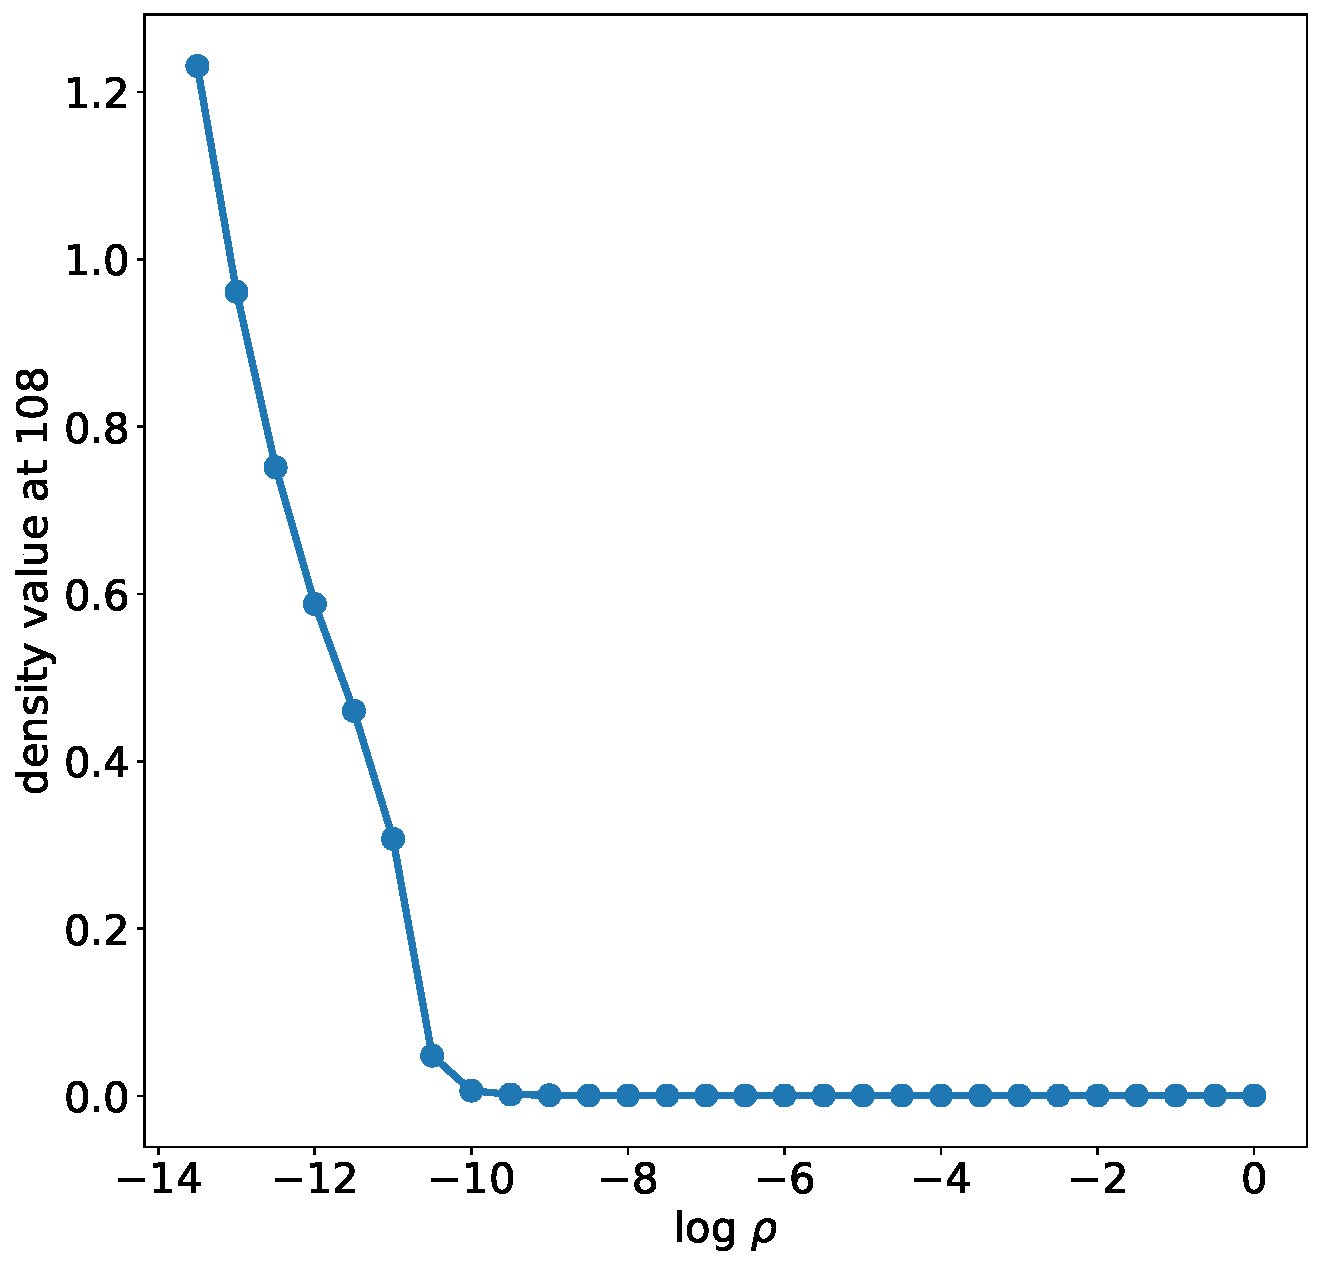
\includegraphics[width=0.6\textwidth]{../plots/density-at-108-vs-log-penalty-Gamma-36.0-2.0.pdf}
	\caption{Density value at $108$ against $\log \rho$.}
	\label{fig-density-val-108-vs-log-pen}
\end{figure}

%Density estimates in Figure \ref{fig-penalized-estimate} confirms our prediction. 
%
%\begin{figure}[t]
%	\centering
%	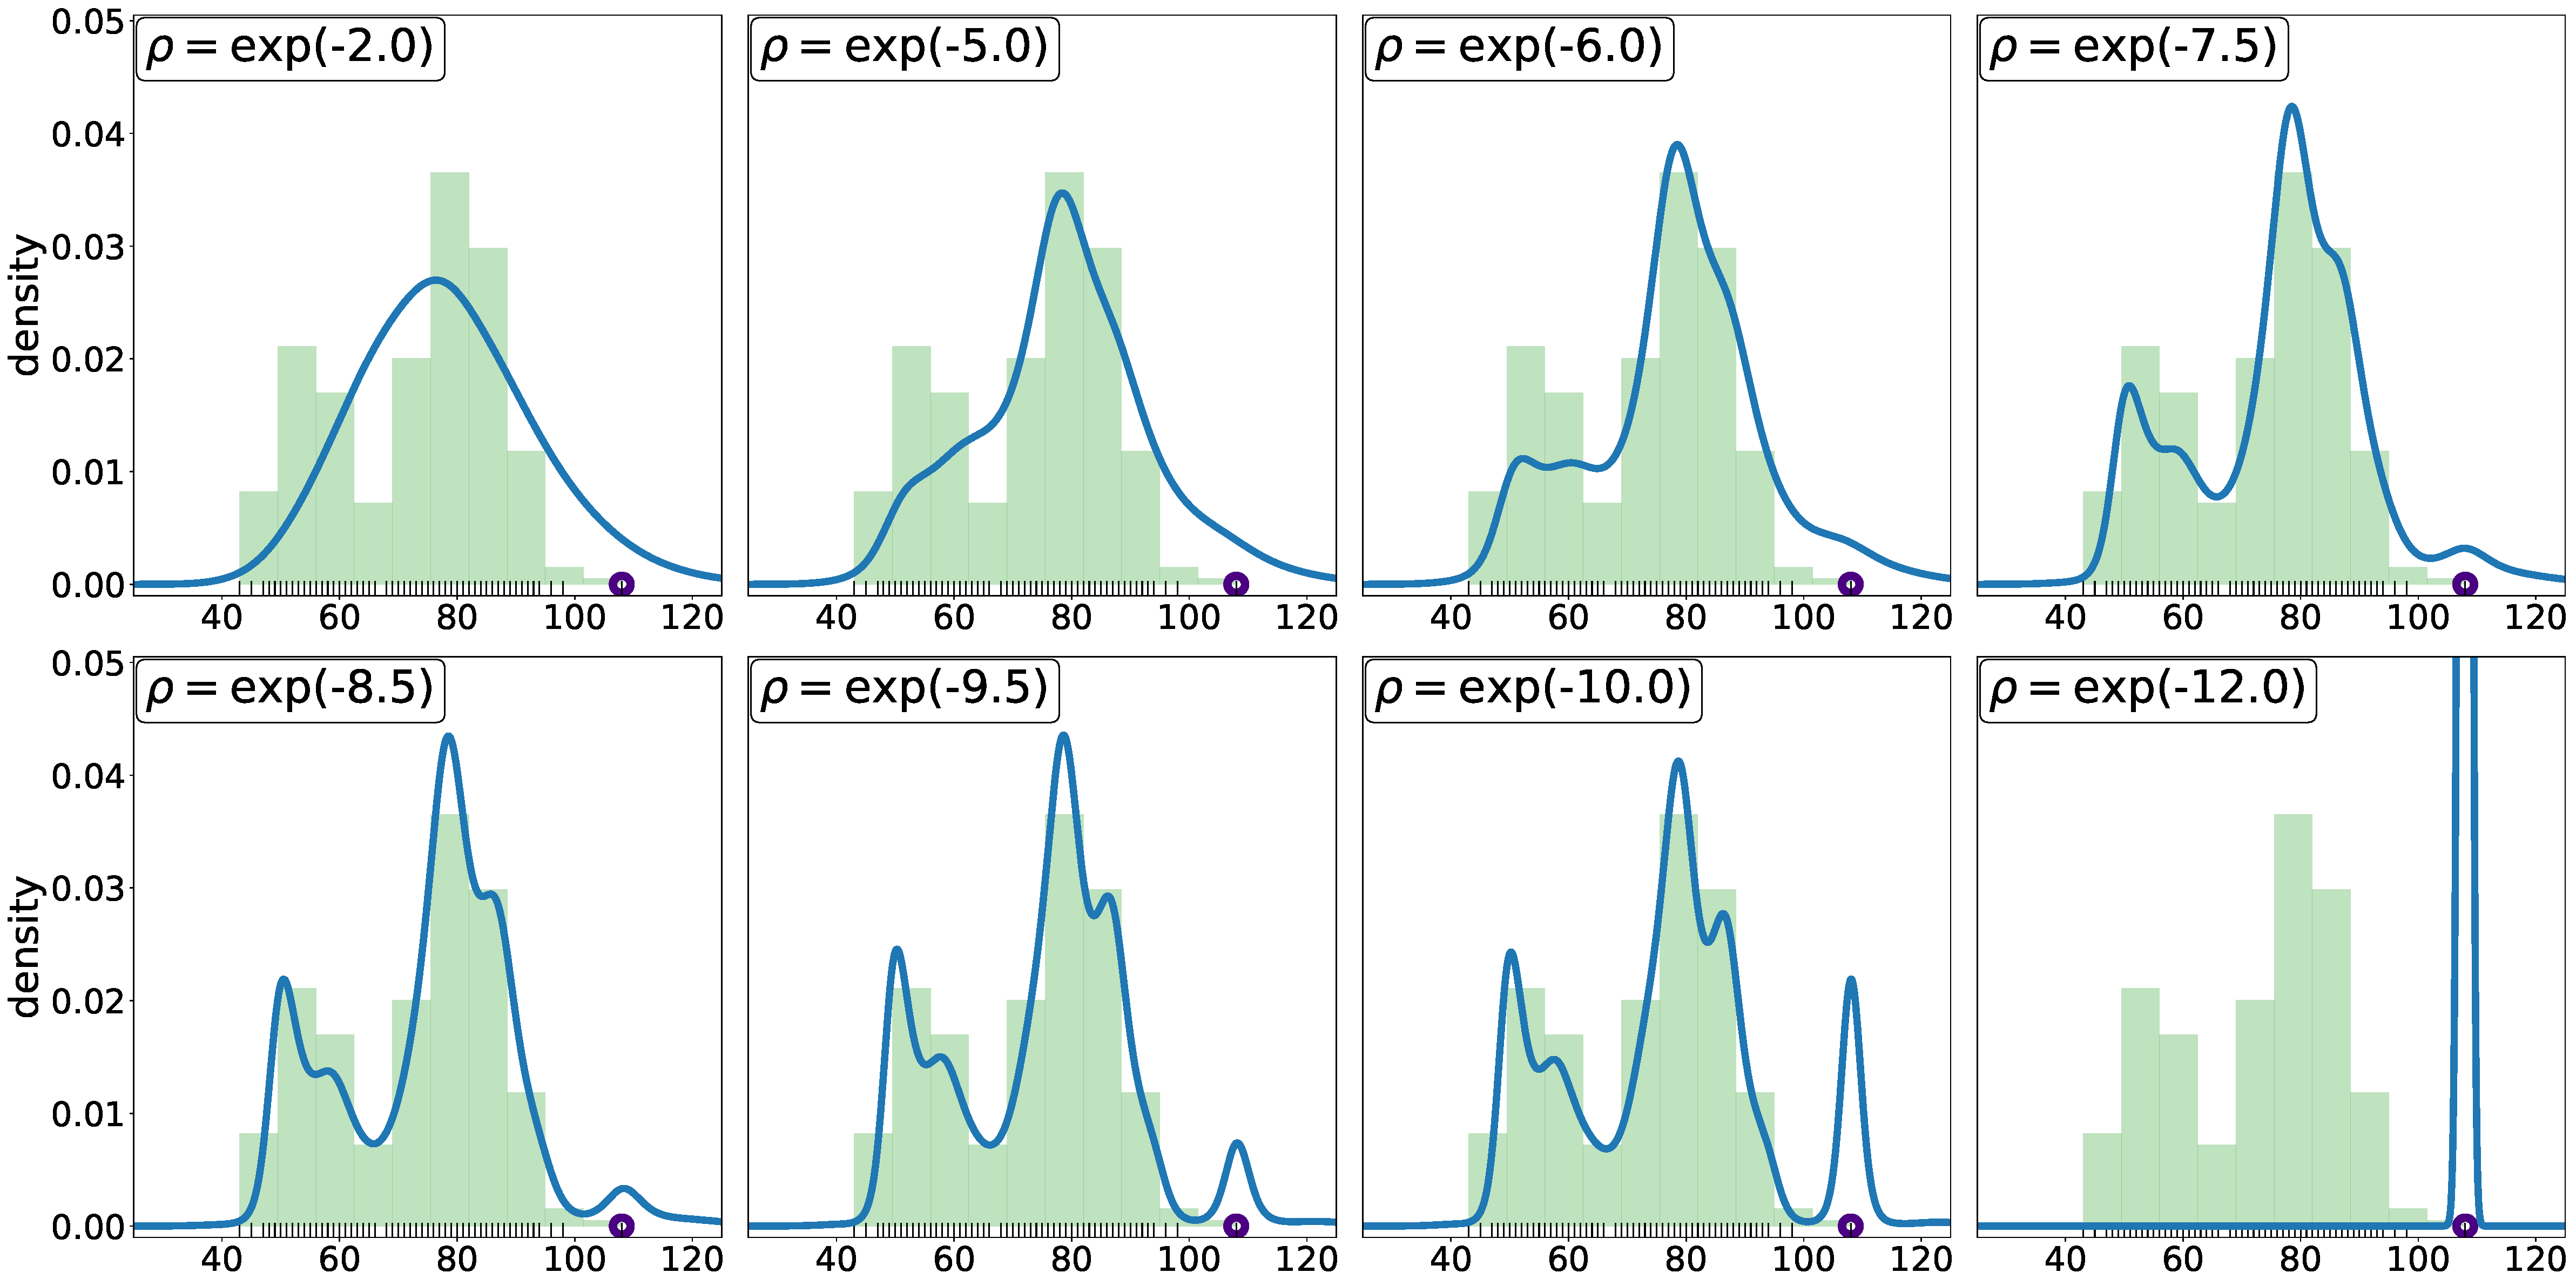
\includegraphics[width=\textwidth]{../plots/waiting-SM-density-estimates-penalized-only-bw=5.0-baseden=Gamma-26-3-entireRKHS.pdf}
%	\caption{Penalized SM density estimates for different values of penalty parameters labeled at the upper left corner. Histogram of data using the Freedman-Diaconis rule is shown in green. The rug plot indicates the location of data and the purple circle indicates the location of the observation 108.}
%	\label{fig-penalized-estimate}
%\end{figure}


\subsection{Comparison through Eigen-decomposition}

We show the similarities of the penalized and early stopping SM density estimators through their eigen-decomposition. 

To this end, we first observe that $\widehat{C}$ has finite rank, and must be a compact operator. In addition, it is self-adjoint. By the Hilbert-Schmidt theorem, there exists a set of eigenfunctions $\sets{\widehat{\psi}_{\nu}}_{\nu=1}^{R}$ that forms an orthonormal basis for $\range \parens{\widehat{C}}$ and $\widehat{C} \widehat{\psi}_{\nu} = \hat{\xi}_{\nu} \widehat{\psi}_{\nu}$ for all $\nu = 1, \cdots, R$, where $\hat{\xi}_1 \ge \hat{\xi}_2 \ge \cdots \ge \hat{\xi}_R > 0$ are the eigenvalues of $\widehat{C}$ and $R < \infty$ denotes the rank of $\widehat{C}$. 

By \eqref{eq-penalized-sm-sol} in Chapter \ref{ch2} and Proposition \ref{prop-commutativity-Pi}, we have 
\begin{align}
	\hat{f}^{\parens{\rho}} = \parens{\widehat{C} + \rho I}^{-1} \hat{z} = & \, \parens{\widehat{C} + \rho I}^{-1} \widehat{C} \hat{g}_1 + \frac{1}{\rho} \hat{z}_2 \nonumber \\ 
	= & \, \sum_{\nu=1}^R \frac{\hat{\xi}_{\nu}}{\hat{\xi}_{\nu} + \rho} \innerp{\hat{g}_1}{\widehat{\psi}_{\nu}}_{\calH} \widehat{\psi}_{\nu} + \frac{1}{\rho} \hat{z}_2, \label{eq-comparison-pen-es-1}
\end{align}
where $\hat{g}_1 \in \calH$ satisfying $\hat{z}_1 = \widehat{C} \hat{g}_1$. In addition, by Proposition \ref{prop-decomposition-ft}, we have 
\begin{align}
	\hat{f}^{\parens{t}} = \tau \sum_{j=0}^{t-1} \parens{I - \tau \widehat{C}}^j \hat{z} = & \, \parens{I - \parens{I - \tau \widehat{C}}^{t}} \hat{g}_1 + t \tau \hat{z}_2 \nonumber \\ 
	= & \, \sum_{\nu=1}^R \parens{1 - \parens{1 - \tau \hat{\xi}_{\nu} }^{t}} \innerp{\hat{g}_1}{\widehat{\psi}_{\nu}}_{\calH} \widehat{\psi}_{\nu} + t \tau \hat{z}_2. \label{eq-comparison-pen-es-2}
\end{align}
Comparing \eqref{eq-comparison-pen-es-1} and \eqref{eq-comparison-pen-es-2}, we see $\hat{f}^{\parens{\rho}}$ and $\hat{f}^{\parens{t}}$ are very similar. The main difference lies in how they regularize the eigenvalues $\sets{\hat{\xi}_{\nu}}_{\nu=1}^R$. In $\hat{f}^{\parens{\rho}}$, the regularization is done through the function $x \mapsto \frac{x}{x + \rho}$, and in $\hat{f}^{\parens{t}}$, the regularization is done through the function $x \mapsto 1 - \parens{1 - \tau x}^t$, for $x > 0$. 

For sufficiently small eigenvalues $\hat{\xi}_{\nu}$, $\frac{\hat{\xi}_{\nu}}{\hat{\xi}_{\nu} + \rho} \approx 0$ and $1 - \parens{1 - \tau \hat{\xi}_{\nu} }^{t} \approx 0$. Therefore, both of them attempt to attenuate the effects of the smaller eigenvalues and let the larger eigenvalues to dominate. 

\subsection{Comparison of Convergence Rates}

So far, we have been focusing more on the similarities of these two density estimators. We stress a key difference of them by examining their convergence rates. 

It has been shown in \textcite{Sriperumbudur-density-estimation-inf-exp-family} that, under the same assumptions as in Theorem \ref{theorem-convergence-rate}, we have $\norm{\hat{f}^{\parens{\rho}} - f_0}_{\calH} = \calO_{p_0} \parens{n^{-\min \braces[\big]{\frac{1}{4}, \frac{\gamma}{2 \parens{\gamma + 1}}}}}$. As the value of $\gamma$ is becoming large, the rate does \emph{not} improve with $\gamma$ and the best possible rate is $n^{-\frac{1}{4}}$, which is achieved when $\gamma = 1$. As we have discussed earlier, the value of $\gamma$ in \ref{assumption-7} indicates the degree of smoothness of $f_0$, and a larger value of $\gamma$ implies that $f_0$ is smoother. However, the rate of $\hat{f}^{\parens{\rho}}$ does \emph{not} really capture this smoothness, since, as soon as $\gamma$ exceeds 1, the rate stabilizes at $n^{-\frac{1}{4}}$ and never improves. This unsatisfactory feature of the penalized SM density estimator is 
%as it does \emph{not} exploit the smoothness of $f_0$. 
called the \emph{saturation phenomenon} in the literature, and has been the main motivation of designing new regularized estimators that do not saturate \parencite{Engl1996-jy,Bauer2007-xq,Lo_Gerfo2008-vv}. 

However, Theorem \ref{theorem-convergence-rate} implies that with the stopping rule $t^*$, we have $\norm{\hat{f}^{\parens{t^* \parens{n}}} - f_0}_{\calH} = \calO_{p_0} \parens{n^{-\frac{\gamma}{2 \parens{\gamma+2}}}}$. Note, in particular, that this rate improves as $\gamma$ increases. As $\gamma \to \infty$, this rate approaches to $n^{-\frac{1}{2}}$, which is faster compared to that in the penalized approach. 


\subsection{Numerical Examples}

We finally compare the early stopping and penalized SM density estimators numerically using the \texttt{waiting} variable in the Old Faithful Geyser dataset. 

The resulting penalized and early stopping SM density estimates with different choices of $\rho$ and $t$ are shown in Figure \ref{fig-earlystopping-pen-estimates}. It is obvious that these two approaches yield very similar density estimates: when the regularization is large (i.e., $\rho$ is large or $t$ is small), density estimates are very similar to $\mu$; as $\rho$ decreases or $t$ increases, density estimates become more reasonable and reveal the bimodal feature of data; if we further decrease $\rho$ or increase $t$ so that there is very small regularization, density estimates contain a bump or become a spike at the isolated observation 108. 

Additional numerical examples confirm our observations above. 

\begin{sidewaysfigure}
	\centering
	
\includegraphics[width=\textwidth]{../plots/waiting-SM-density-estimates-pen-vs-earlystopping-baseden=Gamma-36.0-2.0-entireRKHS-2.pdf}
	\caption{The penalized (first row) and early stopping (second row) SM density estimates with various choices of $\rho$ and $t$, respectively, shown at the upper left corner. Histogram of data with the bin width chosen by the Freedman-Diaconis rule is shown in green. The rug plot indicates the location of data and the purple circle indicates the location of the observation 108.}
	\label{fig-earlystopping-pen-estimates}
\end{sidewaysfigure}

\newpage

\section{Auxiliary Results and Proofs}

%\section{Solution to a Non-homogeneous Difference Equation}
%
%Throughout this section, we repeatedly used the following result on solving a difference equation. 
%
%\begin{proposition}\label{prop-solution-difference-equation}
%	Consider the following linear first-order difference equation
%	\begin{align}\label{eq-diff-equa}
%		x \parens{n+1} = a \parens{n} x \parens{n} + g \parens{n}, 
%	\end{align}
%	with the initial condition $x \parens{0} = x_0$, where we assume that $a \parens{n} \neq 0$ and that both $a \parens{n}$ and $g \parens{n}$ are real-valued functions defined for $n \in \Natural_0$. Then, the unique solution of \eqref{eq-diff-equa} is 
%	\begin{align}
%		x \parens{n+1} = \parens[\Bigg]{\prod_{i=0}^{n} a \parens{i}} x_0 + \sum_{j=0}^{n} \parens[\Bigg]{\prod_{i=j+1}^n a \parens{i}} g \parens{j}, 
%	\end{align}
%	where we let $\prod_{i=k+1}^k a \parens{i} = 1$ and $\sum_{i=k+1}^k a \parens{i} = 0$. 
%\end{proposition}
%
%The proof of Proposition \ref{prop-solution-difference-equation} is omitted but can be found, for example, in \textcite{Elaydi2013-ej}. The main idea of the proof is induction. 

\subsection{Proof of Theorem \ref{thm-grad-widehatJ}}\label{proof-thm-grad-widehatJ}

\begin{proof}[Proof of Theorem \ref{thm-grad-widehatJ}]
	In order to establish the desired result, we first show $\widehat{J}_{\SM}$ is Fr{\'e}chet differentiable over $\calH$ and derive its Frech{\'e}t derivative at $f \in \calH$, and then derive the Fr{\'e}chet gradient operator of $\widehat{J}_{\SM}$ using its definition. 
	
	Let $f \in \calH$ be arbitrary, and $g \in \calH$ be nonzero. 
%	By definition, $\widehat{J}_{\SM}$ is Fr{\'e}chet differentiable at $f \in \calH$ if there exists a bounded linear functional from $\calH$ to $\Real$ such that the following identity holds 
%	\begin{align}
%		\lim_{\norm{g}_{\calH} \to 0} \frac{\abs{\widehat{J}_{\SM} \parens{f + g} - \widehat{J}_{\SM} \parens{f} - \Diff \widehat{J}_{\SM} \parens{f} \parens{g}}}{\norm{g}_{\calH}} = 0, 
%	\end{align}
%	and this bounded linear operator $\Diff \widehat{J}_{\SM} \parens{f}$ is called the Fr{\'e}chet derivative. 
	It is easy to show $\widehat{C}$ is linear. Then, using its linearity, we have 
	\begin{align*}
		\widehat{J}_{\SM} \parens{f + g} - \widehat{J}_{\SM} \parens{f} 
		= & \, \parens[\bigg]{\frac{1}{2} \innerp{f + g}{\widehat{C} \parens{f + g}}_{\calH} - \innerp{f + g}{\hat{z}}_{\calH}} - \parens[\bigg]{\frac{1}{2} \innerp{f}{\widehat{C}f}_{\calH} - \innerp{f}{\hat{z}}_{\calH}} \\ 
		= & \, \innerp{g}{\widehat{C} f - \hat{z}} + \frac{1}{2} \innerp{g}{\widehat{C} g}_{\calH}. 
	\end{align*}
	It then follows 
	\begin{align*}
		0 \le & \, \frac{\abs[\big]{\widehat{J} \parens{f + g} - \widehat{J} \parens{f} - \innerp{g}{\widehat{C} f - \hat{z}}_{\calH}}}{\norm{g}_{\calH}} 
		= \frac{\abs{\frac{1}{2} \innerp{g}{\widehat{C} g}_{\calH}}}{\norm{g}_{\calH}} \\ 
		\stackrel{\mathrm{\parens{i}}}{\le} & \, \frac{1}{2} \norm[\big]{\widehat{C}g}_{\calH} 
		\stackrel{\text{(ii)}}{\le} \frac{1}{2n} \sum_{i=1}^n \sum_{u=1}^d \norm{\partial_u k \parens{X_i, \,\cdot\,}}_{\calH}^2 \norm{g}_{\calH} \\ 
		\stackrel{\text{(iii)}}{\le} & \, \frac{1}{2} d \kappa_2^2 \norm{g}_{\calH} \to 0, \qquad \text{ as } \norm{g}_{\calH} \to 0, 
	\end{align*}
	where we use the Cauchy-Schwartz inequality in (i), the triangle inequality and the Cauchy-Schwartz inequality in (ii), and \ref{assumption-5} in (iii). In addition, note the map $\Diff \widehat{J}_{\SM} \parens{f}: \calH \to \Real$ defined by $ \Diff \widehat{J}_{\SM} \parens{f} \parens{g} = \innerp{g}{\widehat{C}f - \hat{z}}_{\calH}$, for all $g \in \calH$, is linear and bounded, by \ref{assumption-5}. We conclude that $\widehat{J}_{\SM}$ is Frech{\'e}t differentiable at $f \in \calH$ with the Fr{\'e}chet derivative at $f \in \calH$ being 
	\begin{align*}
		\Diff \widehat{J}_{\SM} \parens{f} \parens{g} = \innerp{g}{\widehat{C}f - \hat{z}}_{\calH}, \qquad \text{ for all } g \in \calH. 
	\end{align*}
	Since our choice of $f \in \calH$ here is arbitrary, we conclude that $\widehat{J}_{\SM}$ is Frech{\'e}t differentiable over $\calH$. 
	
	Finally, by the definition of the Fr{\'e}chet gradient, we know $\nabla \widehat{J}_{\SM} \parens{f} = \widehat{C} f - \hat{z}$ for all $f \in \calH$. 
\end{proof}


\subsection{Proof of Theorem \ref{thm-closed-form}}\label{proof-thm-closed-form}

\begin{proof}[Proof of Theorem \ref{thm-closed-form}]
	We prove by induction. In the base case $t = 0$, it is straightforward from \eqref{eq-grad-updates} that 
	\begin{align}\label{eq-proof-thm3-1}
		\hat{f}^{\parens{1}} = & \, \hat{f}^{\parens{0}} - \tau_0 \parens{\widehat{C} \hat{f}^{\parens{0}} - \hat{z}} = \parens{I - \tau_0 \widehat{C}} \hat{f}_{0} + \tau_0 \hat{z}. 
	\end{align}
	Setting $t=0$ in \eqref{eq-closed-form} yields
	\begin{align*}
		\hat{f}^{\parens{1}} = & \, \prod_{i=0}^0 \parens{I - \tau_i \widehat{C}} \hat{f}^{\parens{0}} + \sum_{j=0}^0 \bracks[\Bigg]{\prod_{i=j+1}^0 \parens{I - \tau_i \widehat{C}}} \tau_j \hat{z} 
		= \parens{I - \tau_0 \widehat{C}} \hat{f}^{\parens{0}} + \tau_0 \hat{z}, 
	\end{align*}
	which matches \eqref{eq-proof-thm3-1}. 
	
	Now, we assume \eqref{eq-closed-form} holds for $t = s$ for some $s \in \Natural$, and we wish to show that it also holds for $t = s+1$. By \eqref{eq-grad-updates}, we know that $\hat{f}^{\parens{s+1}} = \parens{I - \tau_s \widehat{C}} \hat{f}^{\parens{s}} + \tau_s \hat{z}$, and by the inductive hypothesis, we know that $\hat{f}^{\parens{s}} = \prod_{i=0}^{s-1} \parens{I - \tau_i \widehat{C}} \hat{f}^{\parens{0}} + \sum_{j=0}^{s-1} \bracks[\big]{\prod_{i=j+1}^{s-1} \parens{I - \tau_i \widehat{C}}} \tau_j \hat{z}$. Hence, 
	\begin{align*}
		\hat{f}^{\parens{s+1}} % = & \, \parens{I - \tau_k \widehat{C}} \hat{f}^{\parens{s}} + \tau_s \hat{z} \\ 
		= & \, \parens{I - \tau_s \widehat{C}} \bracks[\Bigg]{\prod_{i=0}^{s-1} \parens{I - \tau_i \widehat{C}} \hat{f}^{\parens{0}} + \sum_{j=0}^{s-1} \parens[\Bigg]{\prod_{i=j+1}^{s-1} \parens{I - \tau_i \widehat{C}}} \tau_j \hat{z}} + \tau_s \hat{z} \\ 
		= & \, \prod_{i=0}^{s} \parens{I - \tau_i \widehat{C}} \hat{f}^{\parens{0}} + \sum_{j=0}^{s-1} \prod_{i=j+1}^{s} \parens{I - \tau_i \widehat{C}} \tau_j \hat{z} + \prod_{i=s+1}^s \parens{I - \tau_i \widehat{C}} \tau_s \hat{z} \\ 
		= & \, \prod_{i=0}^{s} \parens{I - \tau_i \widehat{C}} \hat{f}^{\parens{0}} + \sum_{j=0}^{s} \parens[\Bigg]{\prod_{i=j+1}^{s} \parens{I - \tau_i \widehat{C}}} \tau_j \hat{z},  
	\end{align*}
	which is the desired result. 
	
	The case of the constant step size is straightforward. 
\end{proof}


\subsection{Proof of Theorem \ref{thm-early-stopping-algo}}\label{proof-theorem-early-stopping-algo}

In order to prove Theorem \ref{thm-early-stopping-algo}, we need the following lemma, which is essentially a generalized version of the binomial theorem with elements in a Hilbert space. 

\begin{lemma}\label{lemma-binomial-C}
	For all $j \in \Natural_0$, we have 
	\begin{align}\label{eq-lemma-bonimial-C-1}
		\parens{I - \tau \widehat{C}}^j = \sum_{\ell=0}^j {j \choose \ell} \parens{-\tau}^{\ell} \widehat{C}^{\ell}. 
	\end{align}
\end{lemma}

\begin{proof}[Proof of Lemma \ref{lemma-binomial-C}]
	We prove by induction. When $j = 0$, the left-hand side of \eqref{eq-lemma-bonimial-C-1} is simply $\parens{I - \tau \widehat{C}}^0 = I$, and the right-hand side is 
	\begin{align*}
		\sum_{\ell=0}^0 {j \choose \ell} \parens{-\tau}^{\ell} \widehat{C}^{\ell} = {0 \choose 0} \parens{-\tau}^{0} \widehat{C}^{0} = I. 
	\end{align*}
	Hence, \eqref{eq-lemma-bonimial-C-1} holds for $j = 0$. 
	
	Now, we assume \eqref{eq-lemma-bonimial-C-1} holds for $j = s$, and we show it also holds for $j = s + 1$. With $j = s+1$, the left-hand side of \eqref{eq-lemma-bonimial-C-1} becomes 
	\begin{align*}
		\parens{I - \tau \widehat{C}}^{s+1} = & \, \parens{I - \tau \widehat{C}} \parens{I - \tau \widehat{C}}^{s} \\ 
		= & \, \parens{I - \tau \widehat{C}} \bracks[\Bigg]{\sum_{\ell=0}^s {s \choose \ell} \parens{-\tau}^{\ell} \widehat{C}^{\ell} } \\ 
		= & \, I \bracks[\Bigg]{\sum_{\ell=0}^s {s \choose \ell} \parens{-\tau}^{\ell} \widehat{C}^{\ell} } - \tau \widehat{C} \bracks[\Bigg]{\sum_{\ell=0}^s {s \choose \ell} \parens{-\tau}^{\ell} \widehat{C}^{\ell} } \\ 
		= & \, \sum_{\ell=0}^s {s \choose \ell} \parens{-\tau}^{\ell} \widehat{C}^{\ell} + \sum_{\ell=0}^s {s \choose \ell} \parens{-\tau}^{\ell + 1} \widehat{C}^{\ell + 1} \\ 
		= & \, I + \sum_{\ell=1}^s {s \choose \ell} \parens{-\tau}^{\ell} \widehat{C}^{\ell} + \sum_{\ell=0}^{s-1} {s \choose \ell} \parens{-\tau}^{\ell + 1} \widehat{C}^{\ell + 1} + {s \choose s} \parens{-\tau}^{s+1} \widehat{C}^{s + 1} \\ 
		= & \, I + \sum_{\ell=1}^s {s \choose \ell} \parens{-\tau}^{\ell} \widehat{C}^{\ell} + \sum_{\ell=1}^{s} {s \choose \ell-1} \parens{-\tau}^{\ell} \widehat{C}^{\ell} + \parens{-\tau}^{s+1} \widehat{C}^{s + 1} \\ 
		= & \, I + \sum_{\ell=1}^s \bracks[\bigg]{{s \choose \ell} + {s \choose \ell-1}} \parens{-\tau}^{\ell} \widehat{C}^{\ell} + \parens{-\tau}^{s+1} \widehat{C}^{s + 1} \\ 
		= & \, {s+1 \choose 0} I + \sum_{\ell=1}^s {s+1 \choose \ell} \parens{-\tau}^{\ell} \widehat{C}^{\ell} + {s+1 \choose s+1} \parens{-\tau}^{s+1} \widehat{C}^{s + 1} \\ 
		= & \, \sum_{\ell=0}^{s+1} {s+1 \choose \ell} \parens{-\tau}^{\ell} \widehat{C}^{\ell}, 
	\end{align*}
	where we use the inductive hypothesis in the second equality. 
\end{proof}


We also need the following lemma which gives an explicit characterization of $\widehat{C}^{\ell} \hat{z}$. 

\begin{lemma}\label{lemma-C-power-z}
	For all $\ell \in \Natural$, we have 
	\begin{align}\label{eq-C-power-z}
		\widehat{C}^{\ell} \hat{z} = \frac{1}{n^{\ell}} \sum_{i=1}^n \sum_{u=1}^d \bracks[\big]{\bG^{\ell-1} \bh}_{\parens{i-1}d+u} \partial_u k \parens{X_i, \,\cdot\,}, 
	\end{align}
	where $\bG \in \Real^{nd \times nd}$ and $\bh \in \Real^{nd}$ are the same as those defined in Theorem \ref{thm-early-stopping-algo}. 
%	the $\parens{\parens{i-1}d+u, \parens{j-1}d+v}$-th entry of $\bG \in \Real^{\parens{nd} \times \parens{nd}}$ is $\innerp{\partial_u k \parens{X_i, \cdot}}{\partial_v k \parens{X_j, \cdot}}_{\calH} = \partial_u \partial_{v+d} k \parens{X_i, X_j}$, and the $\parens{\parens{i-1}d+u}$-th entry of $\bh \in \Real^{nd}$ is 
%	\begin{align*}
%		\innerp{\hat{z}}{\partial_u k \parens{X_i, \,\cdot\,}}_{\calH} = - \frac{1}{n} \sum_{j=1}^n \sum_{v=1}^d \parens[\Big]{\partial_u \partial^2_{v+d} k \parens{X_i, X_j} + \partial_v \log \mu \parens{X_j} \partial_u \partial_{v+d} k \parens{X_i, X_j}}. 
%	\end{align*}
\end{lemma}


\begin{proof}[Proof of Lemma \ref{lemma-C-power-z}]
	First note that, for any $\ell \ge 1$, $\widehat{C}^{\ell} \hat{z}$ resides in $\range \parens{\widehat{C}}$ that contains all functions of the form 
	\begin{align*}
		\widehat{C} g = \frac{1}{n} \sum_{i=1}^n \sum_{u=1}^d \innerp{\partial_u k \parens{X_i, \,\cdot\,}}{g}_{\calH} \partial_u k \parens{X_i, \,\cdot\,}, \qquad \text{ for some } g \in \calH. 
	\end{align*}	
	In other words, all functions in $\range \parens{\widehat{C}}$ can be written as a linear combination of $\partial_u k \parens{X_i, \,\cdot\,}$, for all $i = 1, \cdots, n$ and $u = 1, \cdots, d$. 
	
	We prove \eqref{eq-C-power-z} by induction. Note when $\ell = 1$, the left-hand side of \eqref{eq-C-power-z} is 
	\begin{align*}
		\widehat{C} \hat{z} = & \, \frac{1}{n} \sum_{i=1}^n \sum_{u=1}^d \innerp{\partial_u k \parens{X_i, \,\cdot\,}}{\hat{z}}_{\calH} \partial_u k \parens{X_i, \,\cdot\,} 
		= \frac{1}{n} \sum_{i=1}^n \sum_{u=1}^d \bracks{\bh}_{\parens{i-1}d+u} \partial_u k \parens{X_i, \,\cdot\,} \\ 
		= & \, \frac{1}{n} \sum_{i=1}^n \sum_{u=1}^d \bracks{\bG^{1-1} \bh}_{\parens{i-1}d+u} \partial_u k \parens{X_i, \,\cdot\,}. 
	\end{align*}
	Hence, \eqref{eq-C-power-z} holds for $\ell = 1$. 
	
	Now, suppose that \eqref{eq-C-power-z} holds for $\ell = s$. We want to show it also holds for $\ell = s + 1$. Note the following 
	\begin{align*}
		\widehat{C}^{s+1} \hat{z} = & \, \widehat{C} \parens{\widehat{C}^{s} \hat{z}} \\ 
		= & \, \parens[\bigg]{\frac{1}{n} \sum_{i=1}^n \sum_{u=1}^d \partial_u k \parens{X_i, \,\cdot\,} \otimes \partial_u k\parens{X_i, \,\cdot\,}} \parens[\bigg]{\frac{1}{n^{s}} \sum_{j=1}^n \sum_{v=1}^d \bracks{\bG^{s-1} \bh}_{\parens{j-1}d+v} \partial_v k \parens{X_j, \,\cdot\,}} \\ 
		= & \, \frac{1}{n^{s+1}} \sum_{i=1}^n \sum_{u=1}^d \parens[\bigg]{\sum_{j=1}^n \sum_{v=1}^d \bracks{\bG^{s-1} \bh}_{\parens{j-1}d+v} \innerp{\partial_u k \parens{X_i, \,\cdot\,}}{\partial_v k\parens{X_j, \,\cdot\,}}_{\calH}} \partial_u k \parens{X_i, \,\cdot\,} \\ 
		= & \, \frac{1}{n^{s+1}} \sum_{i=1}^n \sum_{u=1}^d \parens[\bigg]{\sum_{j=1}^n \sum_{v=1}^d \bracks{\bG^{s-1} \bh}_{\parens{j-1}d+v} \partial_u \partial_v k \parens{X_i, X_j}} \partial_u k \parens{X_i, \,\cdot\,} \\ 
		= & \, \frac{1}{n^{s+1}} \sum_{i=1}^n \sum_{u=1}^d \bracks{\bG^{s} \bh}_{\parens{i-1}d+u} \partial_u k \parens{X_i, \,\cdot\,}, 
	\end{align*}
	which is the desired result. 
\end{proof}

We now prove Theorem \ref{thm-early-stopping-algo}. 

\begin{proof}[Proof of Theorem \ref{thm-early-stopping-algo}]
	Since, for $t \in \Natural_0$, we have $\hat{f}^{\parens{t+1}} = \tau \sum_{j=0}^t \parens{I - \tau \widehat{C}}^{j} \hat{z}$, using the results of Lemma \ref{lemma-binomial-C}, we can rewrite it as 
	\begin{align*}
		\hat{f}^{\parens{t+1}} = & \, \tau \sum_{j=0}^t \sum_{\ell=0}^j {j \choose \ell} \parens{-\tau}^{\ell} \widehat{C}^{\ell} \hat{z} \nonumber \\ 
		= & \, \tau \hat{z} + \tau \sum_{j=1}^t \sum_{\ell=0}^j {j \choose \ell} \parens{-\tau}^{\ell} \widehat{C}^{\ell} \hat{z} \nonumber \\ 
		= & \, \tau \hat{z} + \tau \sum_{j=1}^t \bracks[\bigg]{\hat{z} + \sum_{\ell=1}^j {j \choose \ell} \parens{-\tau}^{\ell} \widehat{C}^{\ell} \hat{z}} \nonumber \\ 
		= & \, \tau \parens{t + 1} \hat{z} + \tau \sum_{j=1}^t \sum_{\ell=1}^j {j \choose \ell} \parens{-\tau}^{\ell} \widehat{C}^{\ell} \hat{z}. % \label{eq-ft-iter}
	\end{align*}
	Using Lemma \ref{lemma-C-power-z}, we have 
	\begin{align*}
		\hat{f}^{\parens{t+1}} = & \, \tau \parens{t + 1} \hat{z} + \tau \sum_{j=1}^t \sum_{\ell=1}^j {j \choose \ell} \parens{-\tau}^{\ell} \bracks[\bigg]{\frac{1}{n^{\ell}} \sum_{i=1}^n \sum_{u=1}^d \bracks{\bG^{\ell-1} \bh}_{\parens{i-1}d+u} \partial_u k \parens{X_i, \,\cdot\,}} \nonumber \\ 
		= & \, \tau \parens{t + 1} \hat{z} + \tau \sum_{i=1}^n \sum_{u=1}^d \bracks[\Bigg]{\sum_{j=1}^t \sum_{\ell=1}^j {j \choose \ell} \parens[\bigg]{\frac{\parens{-\tau}^{\ell}}{n^{\ell}} \bG^{\ell-1} \bh}}_{\parens{i-1}d+u} \partial_u k \parens{X_i, \,\cdot\,}. 
	\end{align*}
	This proves \eqref{eq-thm-early-stopping-algo-part1}. 
	
	To prove \eqref{eq-thm-early-stopping-algo-part2}, first note the matrix $\bG$ is the Gram matrix of the set of vectors $\sets{\partial_u k \parens{X_i, \,\cdot\,} \text{ for } i = 1, \cdots, n \text{ and } u = 1, \cdots, d}$, implying that $\bG$ is positive semi-definite. Hence, we can write $\bG = \bQ \bLambda \bQ^{\top}$, where again $\bQ \in \Real^{nd \times nd}$ is an orthogonal matrix and $\bLambda \in \Real^{nd \times nd}$ is a diagonal matrix with the eigenvalues of $\bG$, $\lambda_1 \ge \lambda_2 \ge \cdots \ge \lambda_{nd} \ge 0$, on the diagonal. Hence, 
	\begin{align}
		\sum_{j=1}^t \sum_{\ell=1}^j {j \choose \ell} \parens[\bigg]{\frac{\parens{-\tau}^{\ell}}{n^{\ell}} \bG^{\ell-1} \bh}  \nonumber
		= & \, - \frac{\tau}{n} \sum_{j=1}^t \sum_{\ell=1}^j {j \choose \ell} \parens[\bigg]{\parens[\bigg]{- \frac{\tau}{n}}^{\ell-1} \parens{\bQ \bLambda \bQ^\top}^{\ell-1} \bh} \nonumber \\ 
		= & \, - \frac{\tau}{n} \sum_{j=1}^t \sum_{\ell=1}^j {j \choose \ell} \parens[\bigg]{\parens[\bigg]{- \frac{\tau}{n}}^{\ell-1} \bQ \bLambda^{\ell-1} \bQ^\top \bh} \nonumber \\ 
		= & \, - \frac{\tau}{n} \bQ \bracks[\Bigg]{\sum_{j=1}^t \sum_{\ell=1}^j {j \choose \ell} \parens[\bigg]{- \frac{\tau}{n} \bLambda}^{\ell-1}} \bQ^\top \bh. \label{ft.iter1}
	\end{align}
	Now, since $\bLambda$ is a diagonal matrix, the sum and the power in \eqref{ft.iter1} can be performed only on the diagonal elements. Since, by the binomial theorem, 
	\begin{align*}
		\parens{1 + x}^j = 1 + \sum_{\ell=1}^j {j \choose \ell} x^{\ell}, \qquad \quad \text{ for all } x \in \Real, 
	\end{align*}
	we have, for all $w = 1, \cdots, nd$, if $\lambda_w \neq 0$, 
	\begin{align*}
		\sum_{j=1}^t \sum_{\ell=1}^j {j \choose \ell} \parens[\bigg]{- \frac{\tau}{n} \lambda_{w}}^{\ell-1} = & \, \parens[\bigg]{- \frac{\tau}{n} \lambda_{w}}^{-1} \sum_{j=1}^t \bracks[\Bigg]{\sum_{\ell=1}^j {j \choose \ell} \parens[\bigg]{- \frac{\tau}{n} \lambda_{w}}^{\ell}} \nonumber \\ 
		= & \, \parens[\bigg]{- \frac{\tau}{n} \lambda_{w}}^{-1} \sum_{j=1}^t \bracks[\Bigg]{\parens[\bigg]{1 - \frac{\tau}{n} \lambda_{w}}^j - 1} \nonumber \\ 
		= & \, \parens[\bigg]{- \frac{\tau}{n} \lambda_{w}}^{-1} \parens[\bigg]{1 - \frac{\tau}{n} \lambda_{w}} \frac{1 - \parens[\big]{1 - \frac{\tau}{n} \lambda_{w}}^t}{1 - \parens[\big]{1 - \frac{\tau}{n} \lambda_{w}}} - t \parens[\bigg]{- \frac{\tau}{n} \lambda_{w}}^{-1} \nonumber \\ 
		= & \, - \parens[\bigg]{\frac{n}{\tau \lambda_w}}^{2} \parens[\bigg]{1 - \frac{\tau}{n} \lambda_{w}} \parens[\bigg]{1 - \parens[\Big]{1 - \frac{\tau}{n} \lambda_{w}}^t} + \frac{tn}{\tau \lambda_w}, % \label{power.sum.lambda1}
	\end{align*}
	and, if $\lambda_w = 0$, we have 
	\begin{align*}
		\sum_{j=1}^t \sum_{\ell=1}^j {j \choose \ell} \parens[\bigg]{- \frac{\tau}{n} \lambda_{w}}^{\ell-1} = \sum_{j=1}^t j = \frac{\parens{t+1} t}{2}, % \label{power.sum.lambda2}
	\end{align*}
	which are exactly the diagonal elements of $\widetilde{\bLambda}$ defined in the theorem. Therefore, we have 
	\begin{align*}
		\sum_{j=1}^t \sum_{\ell=1}^j {j \choose \ell} \parens[\bigg]{\frac{\parens{-\tau}^{\ell}}{n^{\ell}} \bG^{\ell-1} \bh} = - \frac{\tau}{n} \bQ \widetilde{\bLambda} \bQ^\top \bh, 
	\end{align*}
	
	In addition, we have 
	\begin{align*}
		\hat{f}^{\parens{t+1}} = & \, \tau \parens{t + 1} \hat{z} + \tau \sum_{i=1}^n \sum_{u=1}^d \bracks[\Bigg]{- \frac{\tau}{n} \bQ \widetilde{\bLambda} \bQ^\top \bh}_{\parens{i-1}d+u} \partial_u k \parens{X_i, \,\cdot\,} \\ 
		= & \, \tau \parens{t + 1} \hat{z} - \frac{\tau^2}{n} \sum_{i=1}^n \sum_{u=1}^d \bracks[\Big]{\bQ \widetilde{\bLambda} \bQ^\top \bh}_{\parens{i-1}d+u} \partial_u k \parens{X_i, \,\cdot\,}, 
	\end{align*}
	which completes the proof. 
\end{proof}


\subsection{Proofs of Results in Section \ref{subsec-smes-limiting-t}}\label{subsection-proof-smes-limiting-t}

\begin{proof}[Proof of Proposition \ref{prop-decomposition-ft}]
	Since we can write $\hat{z} = \hat{z}_1 + \hat{z}_2$ with $\hat{z}_1 = \widehat{C} \hat{g}_1 \in \range \parens{\widehat{C}}$ and $\hat{z}_2 \in \range \parens{\widehat{C}}^{\perp}$, we can write the $\parens{t+1}$-st gradient descent iterate as 
	\begin{align*}
		\hat{f}^{\parens{t+1}} = \parens{I - \tau \widehat{C}} \hat{f}^{\parens{t}} + \tau \parens{\hat{z}_1 + \hat{z}_2} = \parens{I - \tau \widehat{C}} \hat{f}^{\parens{t}} + \tau \widehat{C} \hat{g}_1 + \tau \hat{z}_2. 
	\end{align*}
	Subtracting both sides of the preceding equation by $\hat{g}_1$ yields 
	\begin{align}
		\hat{f}^{\parens{t+1}} - \hat{g}_1 %= & \, \parens{I - \tau \widehat{C}} \hat{f}^{\parens{t}} - \hat{g}_1 + \tau \widehat{C} \hat{g}_1 + \tau \hat{z}_2 \nonumber \\ 
		= & \, \parens{I - \tau \widehat{C}} \parens{\hat{f}^{\parens{t}} - \hat{g}_1} + \tau \hat{z}_2. \label{eq-proof-prop-decomposition-ft-1}
	\end{align}
	Projecting both sides of \eqref{eq-proof-prop-decomposition-ft-1} onto $\range \parens{\widehat{C}}$, we obtain 
	\begin{align*}
		\Pi_{\range \parens{\widehat{C}}} \parens{\hat{f}^{\parens{t+1}} - \hat{g}_1} = & \, \Pi_{\range \parens{\widehat{C}}} \parens[\big]{ \parens{I - \tau \widehat{C}} \parens{\hat{f}^{\parens{t}} - \hat{g}_1} + \tau \hat{z}_2} \nonumber \\
		= & \, \parens{I - \tau \widehat{C}} \Pi_{\range \parens{\widehat{C}}} \parens{\hat{f}^{\parens{t}} - \hat{g}_1} \\ 
		= & \, \parens{I - \tau \widehat{C}}^{t+1} \Pi_{\range \parens{\widehat{C}}} \parens{\hat{f}^{\parens{0}} - \hat{g}_1} \\ 
		= & \, \parens{I - \tau \widehat{C}}^{t+1} \Pi_{\range \parens{\widehat{C}}} \parens{- \hat{g}_1} \\ 
		= & \, - \parens{I - \tau \widehat{C}}^{t+1} \hat{g}_1, 
	\end{align*}
	where we use $\hat{f}^{\parens{0}} = 0$ in the next to last equality and $\hat{g}_1 \in \range \parens{\widehat{C}}$ to obtain the last equality. 
	
	Now, project both sides of \eqref{eq-proof-prop-decomposition-ft-1} onto $\range \parens{\widehat{C}}^{\perp}$, we obtain 
	\begin{align*}
		\Pi_{\range \parens{\widehat{C}}^{\perp}} \parens{\hat{f}^{\parens{t+1}} - \hat{g}_1} = & \, \Pi_{\range \parens{\widehat{C}}^{\perp}} \parens{\hat{f}^{\parens{t}} - \hat{g}_1} + \tau \hat{z}_2 \\ 
		= & \, \Pi_{\range \parens{\widehat{C}}^{\perp}} \parens{\hat{f}^{\parens{0}} - \hat{g}_1} + \parens{t+1} \tau \hat{z}_2 \\
		= & \, \parens{t+1} \tau \hat{z}_2, 
	\end{align*}
	where we again use $\hat{f}^{\parens{0}} = 0$ and $\hat{g}_1 \in \range \parens{\widehat{C}}$. 
	
	Finally, we have 
	\begin{align*}
		\hat{f}^{\parens{t+1}} = & \, \hat{g}_1 + \Pi_{\range \parens{\widehat{C}}} \parens{\hat{f}^{\parens{t+1}} - \hat{g}_1} + \Pi_{\range \parens{\widehat{C}}^{\perp}} \parens{\hat{f}^{\parens{t+1}} - \hat{g}_1} \nonumber \\ 
		= & \, \hat{g}_1 - \parens{I - \tau \widehat{C}}^{t+1} \hat{g}_1 + \tau \parens{t+1} \hat{z}_2 \nonumber \\ 
		= & \, \parens{I - \parens{I - \tau \widehat{C}}^{t+1}} \hat{g}_1 + \tau \parens{t+1} \hat{z}_2, 
	\end{align*}
	which is the desired result. 
\end{proof}


\begin{proof}[Proof of Proposition \ref{prop-hatz1-hatz2-g1}]
	\ref{prop-hatz1-hatz2-g1-1} Since $\hat{z}_1$ is the orthogonal projection of $\hat{z}$ onto $\range \parens{\widehat{C}}$, by the definition of projection, we have 
		\begin{align*}
			\hat{z}_1 = \argmin_{w \in \range \parens{\widehat{C}}} \norm{\hat{z} - w}_{\calH}^2. 
		\end{align*}
	Since $w \in \range \parens{\widehat{C}}$, we can write $w = \sum_{i=1}^n \sum_{u=1}^d \alpha_{\parens{i-1}d+u} \partial_u k \parens{X_i, \,\cdot\,}$ for some $\balpha := \parens{\alpha_{1}, \cdots, \alpha_{nd}}^\top \in \Real^{nd}$. Then, 
	\begin{align*}
		\norm{\hat{z} - w}_{\calH}^2 = & \, \norm[\bigg]{\hat{z} - \sum_{i=1}^n \sum_{u=1}^d \alpha_{\parens{i-1}d+u} \partial_u k \parens{X_i, \,\cdot\,}}_{\calH}^2 \nonumber \\ 
		= & \, \norm{\hat{z}}_{\calH}^2 - 2 \sum_{i=1}^n \sum_{u=1}^d  \alpha_{\parens{i-1}d+u} \innerp{\hat{z}}{ \partial_u k \parens{X_i, \,\cdot\,} }_{\calH} + \norm[\Bigg]{\sum_{i=1}^n \sum_{u=1}^d \alpha_{\parens{i-1}d+u} \partial_u k \parens{X_i, \,\cdot\,}}_{\hil}^2 \nonumber \\ 
		= & \, \norm{\hat{z}}_{\calH}^2 - 2 \balpha^\top \bh + \balpha^\top \bG \balpha. 
	\end{align*}
	Since $\bG$ is a Gram matrix and is positive definite by assumption, the function $\balpha \mapsto \norm{\hat{z}}_{\calH}^2 - 2 \balpha^\top \bh + \balpha^\top \bG \balpha$ is convex and differentiable in $\balpha$. Then, $\balpha^* := \argmin_{\balpha} \sets{\norm{\hat{z}}_{\calH}^2 - 2 \balpha^\top \bh + \balpha^\top \bG \balpha}$ must exist and satisfy the first-order optimality condition $\boldzero = - \bh + \bG \balpha^*$, which is the desired linear system. 

	% If, in particular, $\bG \in \Real^{nd \times nd}$ is invertible, $\balpha^* = \bG^{-1} \bh$. 
		
	\ref{prop-hatz1-hatz2-g1-2} The result is straightforward using the relationship $\hat{z} = \hat{z}_1 + \hat{z}_2$, the definition of $\hat{z}$, the result from \ref{prop-hatz1-hatz2-g1-1}. 
	
	\ref{prop-hatz1-hatz2-g1-3} Since $\hat{g}_1$ belongs to $\range \parens{\widehat{C}}$ and satisfies the relationship $\hat{z}_1 = \widehat{C} \hat{g}_1$, we let $\hat{g}_1 = \sum_{j=1}^n \sum_{v=1}^d \beta_{\parens{j-1}d+v}^* \partial_j k \parens{X_b, \,\cdot\,}$ and must have 
	\begin{align*}
		\hat{z}_1 = \widehat{C} \hat{g}_1 = & \, \bracks[\Bigg]{\frac{1}{n} \sum_{i=1}^n \sum_{u=1}^d \partial_u k \parens{X_i, \,\cdot\,} \otimes \partial_u k \parens{X_i, \,\cdot\,}} \parens[\Bigg]{\sum_{j=1}^n \sum_{v=1}^d \beta_{\parens{j-1}d+v}^* \partial_v k \parens{X_j, \,\cdot\,}} \nonumber \\ 
		= & \, \sum_{i=1}^n \sum_{u=1}^d \bracks[\Bigg]{ \frac{1}{n} \sum_{j=1}^n \sum_{v=1}^d \beta_{\parens{j-1}d+v}^* \partial_u \partial_{v+d} k \parens{X_i, X_j}} \partial_u k \parens{X_i, \,\cdot\,}. 
	\end{align*}
	It follows that, for all $i = 1, \cdots, n$ and $u = 1, \cdots, d$, 
	\begin{align*}
		\alpha^*_{\parens{i-1}d+u} = \frac{1}{n} \sum_{j=1}^n \sum_{v=1}^d \beta_{\parens{j-1}d+v}^* \partial_u \partial_{v+d} k \parens{X_i, X_j}. 
	\end{align*}
	In other words, $\bbeta^* := \parens{\beta_1^*, \cdots, \beta_{nd}^*}^\top \in \Real^{nd}$ must satisfy $\frac{1}{n} \bG \bbeta^* = \balpha^*$. 
\end{proof}


\begin{proof}[Proof of Proposition \ref{proposition-bound-hatz1}]
	Recall from Proposition \ref{prop-decomposition-ft} that $\hat{f}_1^{\parens{t+1}} = \parens{I - \parens{I - \tau \widehat{C}}^t} \hat{g}_1$. Then, note the following 
	\begin{align*}
		\abs{\innerp{\hat{f}_1^{\parens{t+1}}}{k \parens{x, \,\cdot\,}}_{\calH}} = & \, \abs[\big]{\innerp{\parens{I - \parens{I - \tau \widehat{C}}^t} \hat{g}_1}{k \parens{x, \,\cdot\,}}_{\calH}} \\ 
		\stackrel{\text{(i)}}{\le} & \, \norm{I - \parens{I - \tau \widehat{C}}^t} \norm{\hat{g}_1}_{\calH} \norm{k \parens{x, \,\cdot\,}}_{\calH} \\ 
		 \stackrel{\text{(ii)}}{\le} & \, \norm{\hat{g}_1}_{\calH} \sup_{x \in \calX} \norm{k \parens{x, \,\cdot\,}}_{\calH} \\ 
		 \stackrel{\text{(iii)}}{\le} & \, \kappa_1 \norm{\hat{g}_1} =: M. 
	\end{align*}
	In the development above, (i) follows from the Cauchy-Schwartz inequality and the sub-multiplicative property and the definition of the operator norm. Due to \ref{assumption-limiting-2}, $\norm{I - \parens{I - \tau \widehat{C}}^t} \le 1$ for all $t$ and (ii) holds. Finally, (iii) follows from \ref{assumption-2-2-bdd-kernel}. 
\end{proof}

We are now ready to prove Theorem \ref{thm-limiting-density-t}. 

\begin{proof}[Proof of Theorem \ref{thm-limiting-density-t}]
	Let $\hat{z}_2 \parens{x} := \innerp{\hat{z}_2}{ k \parens{x, \,\cdot\,}}_{\calH}$ for all $x \in \calX$. Notice that
	\begin{align*}
		q_{\hat{f}^{\parens{t}}} \parens{x^*} = \frac{\mu \parens{x^*} \exp \parens[\big]{\innerp{\parens{I - \parens{I - \tau \widehat{C}}^t} \hat{g}_1}{k \parens{x^*, \,\cdot\,}}_{\calH} + \tau t \hat{z}_2 \parens{x^*}}}{\int_{\calX} \mu \parens{x} \exp \parens[\big]{\innerp{\parens{I - \parens{I - \tau \widehat{C}}^t} \hat{g}_1}{k \parens{x, \,\cdot\,}}_{\calH} + \tau t \hat{z}_2 \parens{x}} \diff x}. 
	\end{align*}
	Using Proposition \ref{proposition-bound-hatz1}, we can bound $q_{\hat{f}^{\parens{t}}} \parens{x^*}$ from below by 
	\begin{align}\label{proof-thm-limiting-ft-1}
		q_{\hat{f}^{\parens{t}}} \parens{x^*} \ge \frac{ \mu \parens{x^*} \exp \parens[\big]{- M + t \tau \hat{z}_2 \parens{x^*}}}{\int_{\calX} \mu \parens{x} \exp \parens[\big]{M + t \tau \hat{z}_2 \parens{x}} \diff x} = \frac{\exp\parens{-2M} \mu \parens{x^*}}{\int_{\calX} \mu \parens{x} \frac{\exp \parens{t \tau \hat{z}_2 \parens{x} }}{\exp \parens{ t \tau \hat{z}_2 \parens{x^*}}} \diff x}, 
	\end{align}
	where the last equality follows by dividing both the numerator and the denominator by $\exp \parens{t \tau \hat{z}_2 \parens{x^*}}$. 
	
	Since $\hat{z}_2 \parens{x^*} \ge \hat{z}_2 \parens{x}$ for all $x \in \calX$, it follows that 
	\begin{align*}
		\frac{\exp \parens{ t \tau \hat{z}_2 \parens{x}}}{\exp \parens{ t \tau \hat{z}_2 \parens{x^*}}} = \parens[\bigg]{\frac{\exp \parens{ \tau \hat{z}_2 \parens{x}}}{\exp \parens{\tau \hat{z}_2 \parens{x^*}}}}^t \le 1, 
	\end{align*}
	and the equality holds if and only if $x = x^*$, by \ref{assumption-limiting-1}. Then, for all $x \in \calX$ and all $t \in \Natural$, 
	\begin{align*}
		\abs[\bigg]{\mu \parens{x} \parens[\bigg]{\frac{\exp\parens{\tau \hat{z}_2 \parens{x}}}{\exp \parens{\tau \hat{z}_2 \parens{x^*} }}}^t} \le \mu \parens{x}. 
	\end{align*}
	In addition, since $\mu$ is a pdf over over $\calX$ by \ref{assumption-2-4-base-density}, an application of Lebesgue's dominated convergence theorem yields 
	\begin{align*}
		\lim_{t \to \infty} \int_{\calX} \mu \parens{x} \parens[\bigg]{\frac{\exp \parens{\tau \hat{z}_2 \parens{x}}}{\exp \parens{\tau \hat{z}_2 \parens{x^*} }}}^t \diff x 
		= & \, \int_{\calX} \mu \parens{x} \lim_{t \to \infty} \parens[\bigg]{\frac{\exp \parens{\tau \hat{z}_2 \parens{x}}}{\exp \parens{\tau \hat{z}_2 \parens{x^*}}}}^t \diff x \\ 
		= & \, \int_{\calX} \mu \parens{x} \indic_{\sets{x^*}} \parens{x} \, \diff x = 0, 
	\end{align*}
	where $\indic_S$ is the indicator function for the set $S$. 
	
	Taking the limit of $t \to \infty$ of both sides of \eqref{proof-thm-limiting-ft-1}, we have 
	\begin{align*}
		\lim_{t \to \infty} q_{\hat{f}^{\parens{t}}} \parens{x^*} \ge \frac{\exp \parens{-2M} \mu \parens{x^*}}{\lim_{t \to \infty} \int_{\calX} \mu \parens{x} \parens[\big]{\frac{\exp \parens{\tau \hat{z}_2 \parens{x} }}{\exp \parens{\tau \hat{z}_2 \parens{x^*}}}}^t \diff x} = \infty, 
	\end{align*}
	since the numerator is strictly positive by \ref{assumption-2-4-base-density} and the denominator approaches to 0 as $t \to \infty$. 
\end{proof}


\subsection{Proof of Theorem \ref{theorem-convergence-rate}}\label{proof-theorem-convergence-rate}

\begin{proof}[Proof of Theorem \ref{theorem-convergence-rate}]
	Based on the inequality \eqref{eq-sample-plus-approx-errors} and Theorems \ref{theorem-approx-error} and \ref{theorem-sample-error}, we know that with probability at least $1 - \delta$ for $\delta \in \parens{0, 1}$, the following inequality holds 
	\begin{align}\label{eq-stopping-time-inequality}
		\norm{\hat{f}^{\parens{t}} - f_0}_{\hil} \le C_1 \frac{t^2}{\sqrt{n}} + C_2 t^{-\gamma}, 
	\end{align}
	where $C_1$ and $C_2$ are constants defined in the statement of the theorem and come from the upper bounds of the sample error and the approximation error, respectively. Let the stopping rule be $t^* \parens{n} = \ceil{n^{\beta}}$, the smallest integer greater than or equal to $n^{\beta}$ for some $\beta > 0$. Plugging this $t^* \parens{n}$ into the RHS of \eqref{eq-stopping-time-inequality}, we essentially obtain the following function of $\beta$, 
	\begin{align*}
		h \parens{\beta} := C_1 n^{2 \beta - 1/2} + C_2 n^{-\gamma \beta}. 
	\end{align*} 
	By elementary calculus, $h$ achieves the minimum at $\beta^* := \frac{1}{2\parens{\gamma + 2}}$. 

	As a consequence, assuming $n^{\beta^*} \le t^*\parens{n} = \ceil{n^{\beta^*}} = \eta n^{\beta^*} \le n^{\beta^*} + 1$ for some $\eta \in \bracks{1, 2}$, we have 
	\begin{align*}
		\norm{\hat{f}^{\parens{t}} - f_0}_{\calH} \le & \, C_1 \frac{\parens{\eta n^{\beta^*}}^{2}}{\sqrt{n}} + C_2 \parens{\eta  n^{\beta^*}}^{-\gamma} \\ 
		\le & \, C_1 \eta^2 n^{2 \beta^* - \frac{1}{2}} + C_2 \eta^{-\gamma} n^{-\gamma \beta^*} \\ 
		\le & \, \parens{4 C_1 + C_2} n^{-\frac{\gamma}{2 \parens{\gamma+2}}}. 
	\end{align*}
	This completes the proof. 
\end{proof}

\subsection{Proof of Theorem \ref{theorem-approx-error}}\label{proof-theorem-approx-error}

In order to prove Theorem \ref{theorem-approx-error}, we first need the following two lemmas: one describes the relationship between $f_0$ and $z$, which is one part of Theorem 4(ii) by \textcite{Sriperumbudur-density-estimation-inf-exp-family}, and the other one gives an expression of $f^{\parens{t}} - f_0$ that is easier to work with. 

\begin{lemma}[\cite{Sriperumbudur-density-estimation-inf-exp-family}, Theorem 4(ii)]\label{lemma-Cf=z}
	Under \ref{assumption-2-1-inf-dim} - \ref{assumption-2-4-base-density} in Chapter \ref{ch2} and \ref{assumption-1} - \ref{assumption-7}, we have $C f_0 = z$. 
\end{lemma}

\begin{lemma}\label{lemma-approx-error-expression}
	Assume $f^{\parens{0}} = 0$. For all $t \in \Natural_0$, $f^{\parens{t}} - f_0 = - \parens{I - \tau C}^{t} f_0$. 
\end{lemma}

\begin{proof}[Proof of Lemma \ref{lemma-approx-error-expression}]
	Note, when $t = 0$, the desired result holds obviously. 
	
	Now, let $t \in \Natural$. By the relationship $f^{\parens{t}} = f^{\parens{t-1}} - \tau \parens{C f^{\parens{t-1}} - z}$ and Lemma \ref{lemma-Cf=z}, we have 
	\begin{align*}
		f^{\parens{t}} = f^{\parens{t-1}} - \tau \parens{C f^{\parens{t-1}} - C f_0} = f^{\parens{t-1}} - \tau C \parens{f^{\parens{t-1}} - f_0}. 
	\end{align*}
	Subtracting both sides by $f_0$ yields 
	\begin{align*}
		f^{\parens{t}} - f_0 = f^{\parens{t-1}} - f_0 - \tau C \parens{f^{\parens{t-1}} - f_0} 
		= & \, \parens{I - \tau C} \parens{f^{\parens{t-1}} - f_0} \\ 
		= & \, \parens{I - \tau C}^{t} \parens{f^{\parens{0}} - f_0}. 
	\end{align*}
	The desired result follows since $f^{\parens{0}} = 0$. 
\end{proof}

We now prove Theorem \ref{theorem-approx-error}. 

\begin{proof}[Proof of Theorem \ref{theorem-approx-error}]
	By Lemma \ref{lemma-approx-error-expression}, we have $\norm{f^{\parens{t}} - f_0}_{\hil} = \norm{\parens{I - \tau C}^t f_0}_{\hil}$. By the relationship $C^{\gamma} g_0 = f_0$ in \ref{assumption-7}, we have 
	\begin{align*}
		\norm{f^{\parens{t}} - f_0 }_{\calH} = \norm{ \parens{I - \tau C}^t C^{\gamma} g_0}_{\calH} 
		\le \norm{ \parens{I - \tau C}^t C^{\gamma}} \norm{g_0}_{\calH}. 
	\end{align*}
	
	Next, we need to find an upper bound for the operator norm of $\parens{I - \tau C}^t C^{\gamma}$. Since $C$ is a compact self-adjoint operator \parencite[Theorem 4(i) in][]{Sriperumbudur-density-estimation-inf-exp-family}, with an application of the Hilbert-Schmidt Theorem, we have, 
	\begin{align*}
		C f = \sum_{\nu=1}^{\infty} \xi_{\nu} \innerp{f}{\psi_\nu}_{\calH} \psi_\nu, \qquad \quad \text{ for all } f \in \hil, 
	\end{align*}
	where $\sets{\psi_{\nu}}_{\nu=1}^{\infty}$ are the eigenvectors of $C$ that form an orthonormal basis of $\overline{\range \parens{C}}$ and $\sets{\xi_{\nu}}_{\nu=1}^{\infty}$ are corresponding eigenvalues satisfying $\lim_{\nu \to \infty} \xi_{\nu} = 0$ and $C \psi_{\nu} = \xi_{\nu} \psi_{\nu}$ for all $\nu \in \Natural$. It follows that 
	\begin{align}
		\norm{ \parens{I - \tau C}^t C^{\gamma}} \le & \, \sup_{\nu} \braces[\big]{ \parens{1 - \tau \xi_{\nu}}^t \xi_{\nu}^{\gamma}} \nonumber 
		= \sup_{\nu} \exp \parens[\big]{t \log \parens{1 - \tau \xi_{\nu}} + \gamma \log \xi_{\nu}} \nonumber \\ 
		\le & \, \sup_{\nu} \exp \parens[\big]{ - t \tau \xi_{\nu} + \gamma \log \xi_{\nu}}, \label{max.lambda}
	\end{align}
	where the last inequality follows from the basic inequality $\log \parens{1+x} \le x$ for all $x > - 1$. Also, note that $\log \parens{1 - \tau \xi_{\nu}}$ is well-defined since $\tau < 1 / \parens{d\kappa_2^2} \le 1 / \norm{C}$ so that $\tau \xi_{\nu} < 1$ for all $\nu \in \Natural$. 

	Define the function $h \parens{x} = - \tau t x + \gamma \log x$ for all $x > 0$ and we maximize $h$. By elementary calculus, $h$ achieves the maximum at $x^* = \frac{\gamma}{\tau t} > 0$ and the maximum value is $h \parens{x^*} = -\gamma + \gamma \log \parens{\frac{\gamma}{\tau t}}$. Plugging $h \parens{x^*}$ back to \eqref{max.lambda}, we have 
	\begin{align}
		\norm{ \parens{I - \tau C}^t C^{\gamma}} \le \parens[\bigg]{\frac{\gamma}{\tau e t}}^{\gamma}, 
	\end{align}
	and the desired result follows. 
\end{proof}


\subsection{Proof of Theorem \ref{theorem-sample-error}}\label{proof-theorem-sample-error}

In order to prove Theorem \ref{theorem-sample-error}, we first need the following proposition that gives an equivalent expression of $\hat{f}^{\parens{t}}$ that links operators $\widehat{C}$ and $C$. 

\begin{proposition}\label{prop-equivalent-sample-updates}
	The sample-version gradient descent updates can be written as 
	\begin{align*}
		\hat{f}^{\parens{t+1}} = \parens{I - \tau C}^{t+1} \hat{f}^{\parens{0}} + \tau \sum_{j=0}^t \parens{I - \tau C}^{t - j} \parens[\big]{\parens{C - \widehat{C}} \hat{f}_j + \hat{z}}. 
	\end{align*}
\end{proposition}

\begin{proof}[Proof of Proposition \ref{prop-equivalent-sample-updates}]
	We start from \eqref{eq-grad-updates} and note 
	\begin{align*}
		\hat{f}^{\parens{t+1}} = & \, \parens{I - \tau \widehat{C}} \hat{f}^{\parens{t}} + \tau \hat{z} \\ 
		= & \, \parens{I - \tau C + \tau C - \tau \widehat{C}} \hat{f}^{\parens{t}} + \tau \hat{z} \\ 
		= & \, \parens{I- \tau C} \hat{f}^{\parens{t}} + \tau \parens{\parens{C - \widehat{C}} \hat{f}^{\parens{t}} + \hat{z}}. 
	\end{align*}
	Now, we obtain a non-homogeneous linear first-order difference equation. The rest can be proved by induction and is similar to the proof of Theorem \ref{thm-closed-form}, which we omit. 
\end{proof}

We also need the following lemma, which is an extension of the Hoeffding inequality to random variables in a Hilbert space. It will help us to obtain probabilistic upper bounds for $\norm{\widehat{C} - C}$ and $\norm{\hat{z} - z}_{\calH}$. 

\begin{lemma}[Hoeffding-Pinelis inequality]\label{lemma-hoeffding}
	Let $\sets{W_i}_{i=1}^n$ be an independent random sequence of mean zero in a separable Hilbert space $\hil$ with the norm $\norm{}_{\calH}$ such that, for all $i = 1, \cdots, n$, $\norm{W_i}_{\calH} \le c_i < \infty$ almost surely. Then, for any $\varepsilon > 0$, 
	\begin{align*}
		\Pr \parens[\Bigg]{\norm[\bigg]{\sum_{i=1}^n W_i}_{\calH} \ge \varepsilon} \le 2 \exp \parens[\bigg]{- \frac{\varepsilon^2}{2 \sum_{i=1}^n c_i^2}}. 
	\end{align*}
	Equivalently, with probability at least $1 - \delta$ where $\delta \in \parens{0, 1}$, we have 
	\begin{align*}
		\norm[\Bigg]{\sum_{i=1}^n W_i}_{\hil} \le \sqrt{2 \parens[\Bigg]{\sum_{i=1}^n c_i^2} \log \parens[\bigg]{\frac{2}{\delta}}}. 
	\end{align*}
	If, in particular, $c_i \equiv c > 0$ for all $i$, then with probability at least $1 - \delta$ for $\delta \in \parens{0, 1}$, we have 
	\begin{align*}
		\frac{1}{n} \norm[\Bigg]{\sum_{i=1}^n W_i}_{\calH} \le c \sqrt{\frac{2}{n} \log \parens[\bigg]{\frac{2}{\delta}}}. 
	\end{align*}
\end{lemma}

In order to use Lemma \ref{lemma-hoeffding} to bound $\norm{\widehat{C} - C}$ and $\norm{\hat{z} - z}_{\calH}$, we need to show the (almost surely) boundedness of several quantities, which we now state and prove. 

\begin{lemma}\label{lemma-population-C-z-bounds}
	Under \ref{assumption-1} - \ref{assumption-5}, the operator $C: \calH \to \calH$ defined in \eqref{eq-C-def} is a Hilbert-Schmidt operator with $\norm{C}_{\mathrm{HS}} \le d \kappa_2^2$, where $\norm{}_{\mathrm{HS}}$ denotes the Hilbert-Schmidt norm, and the function $z$ defined in \eqref{eq-z-def} satisfies $\norm{z}_{\calH} \le d \parens{\kappa_3 + \kappa_4}$. 
\end{lemma}

A brief introduction to the Hilbert-Schmidt operator can be found in Section \ref{section-bdd-linear-operator} in Appendix \ref{app1}. 

\begin{proof}[Proof of Lemma \ref{lemma-population-C-z-bounds}]
	In the proof of Theorem 4 in \textcite{Sriperumbudur-density-estimation-inf-exp-family}, they have shown that the operator $C: \calH \to \calH$ is of trace class and 
	\begin{align*}
		\trace \parens{C} = \int_{\calX} p_0 \parens{x} \sum_{u=1}^d \partial_u \partial_{u+d} k \parens{x, x} \diff x \stackrel{\text{(i)}}{\le} d \kappa_2^2 < \infty, 
	\end{align*}
	where (i) follows from \ref{assumption-5}. By the relationship between the Hilbert-Schmidt norm and the trace (see Proposition \ref{prop-hs-property}\ref{prop-hs-property-c} in Appendix \ref{app1}), we conclude that $\norm{C}_{\mathrm{HS}} \le \trace \parens{C} \le d \kappa_2^2$. 
	
	As for the result on $z$, using Proposition \ref{prop-properties-bochcher-integral}\ref{prop-properties-bochcher-integral-b} in Appendix \ref{app1}, we have  
	\begin{align*}
		\norm{z}_{\calH} \le & \, \sum_{u=1}^d \int_{\calX} p_0 \parens{x} \parens[\Big]{\abs{{\partial_u \log \mu \parens{x}}} \norm{\partial_u k \parens{x, \,\cdot\,}}_{\calH} + \norm{\partial_u^2 k \parens{x, \,\cdot\,}}_{\calH}} \diff x 
		\stackrel{\text{(ii)}}{\le} d \parens{\kappa_3 + \kappa_4}, 
	\end{align*}
	where the inequality (ii) is again due to \ref{assumption-5}. 
\end{proof}

\begin{lemma}\label{lemma-sample-C-z-bounds}
	Under \ref{assumption-1} - \ref{assumption-5}, for all $i = 1, \cdots, n$, the operator $\widehat{C}_i: \hil \to \hil$ defined by 
	\begin{align}\label{eq-def-Ci}
		\widehat{C}_i := \sum_{u=1}^d \partial_u k \parens{X_i, \,\cdot\,} \otimes \partial_u k \parens{X_i, \,\cdot\,}
	\end{align}
	is a Hilbert-Schmidt operator with $\norm{\widehat{C}_i}_{\mathrm{HS}} \le d \kappa_2^2$, and the function $\hat{z}_i$ defined by 
	\begin{align}\label{eq-def-zi}
		\hat{z}_i := - \sum_{u=1}^d \parens[\big]{\partial_u \log \mu \parens{X_i} \partial_u k \parens{X_i, \,\cdot\,} + \partial_u^2 k \parens{X_i, \,\cdot\,}} \in \calH
	\end{align}
	satisfies $\norm{\hat{z}_i}_{\calH} \le d \parens{\kappa_3 + \kappa_4}$. In addition, we have $\norm{\widehat{C}}_{\mathrm{HS}} \le d \kappa_2^2$ and $\norm{\hat{z}}_{\calH} \le d \parens{\kappa_3 + \kappa_4}$. 
\end{lemma}

\begin{proof}[Proof of Lemma \ref{lemma-sample-C-z-bounds}]
	We first show $\widehat{C}_i$ is a Hilbert-Schmidt operator. Pick an arbitrary orthonormal basis $\sets{e_\ell}_{\ell \in \Natural}$ of $\hil$ and an arbitrary $i \in \sets{1, \cdots, n}$. Then, note the following 
	\begin{align*}
		\norm{\widehat{C}_i}_{\mathrm{HS}}^2 = \sum_{\ell=1}^{\infty} \norm{\widehat{C}_i e_{\ell}}_{\hil}^2 = & \, \sum_{\ell=1}^{\infty} \norm[\Bigg]{\sum_{u=1}^d \partial_u e_\ell \parens{X_i} \partial_u k \parens{X_i, \,\cdot\,} }_{\calH}^2 \\ 
		\stackrel{\text{(i)}}{\le} & \, d \sum_{\ell=1}^{\infty} \sum_{u=1}^d \abs{\partial_u e_\ell \parens{X_i}}^2 \norm{\partial_u k \parens{X_i, \,\cdot\,}}_{\calH}^2 \\ 
		\stackrel{\text{(ii)}}{=} & \, d \sum_{u=1}^d \bracks[\Bigg]{\sum_{\ell=1}^{\infty} \abs[\big]{\innerp{\partial_u k \parens{X_i, \,\cdot\,}}{e_\ell }_{\calH}}^2} \norm{\partial_u k \parens{X_i, \,\cdot\,}}_{\calH}^2 \\ 
		\stackrel{\text{(iii)}}{=} & \, d \sum_{u=1}^d \norm{\partial_u k \parens{X_i, \,\cdot\,} }_{\hil}^2 \norm{\partial_u k \parens{X_i, \,\cdot\,} }_{\calH}^2 \\ 
		\stackrel{\text{(iv)}}{=} & \, d \sum_{u=1}^d \parens{\partial_u \partial_{u+d} k \parens{X_i, X_i} }^2 \\ 
		\stackrel{\text{(v)}}{\le} & \, d^2 \kappa_2^4 < \infty, 
	\end{align*}
	and hence, $\norm{\widehat{C}_i}_{\mathrm{HS}} \le d \kappa_2^2$. In the derivation above, (i) is due to the Cauchy-Schwartz inequality. We interchange the sums in (ii) due to the Tonelli-Fubini Theorem. An application of the Parseval's identity yields the equality (iii). We use the reproducing property of the partial derivatives of $k$ in (iv). We use \ref{assumption-5} in (v). 

	As for the result on $\hat{z}_i$, for any $i \in \sets{1, \cdots, n}$, we use \ref{assumption-6} and have 
	\begin{align*}
		\norm{\hat{z}_i}_{\hil} \le \sum_{u=1}^d \parens[\Big]{\abs{\partial_u \log \mu \parens{X_i}} \norm{\partial_u k \parens{X_i, \,\cdot\,} }_{\calH} + \norm{\partial_u^2 k \parens{X_i, \,\cdot\,} }_{\hil}} \le d \parens{\kappa_3 + \kappa_4}. 
	\end{align*}
	
	The bounds on $\norm{\widehat{C}}_{\mathrm{HS}}$ and $\norm{\hat{z}}_{\calH}$ easily follows by the triangle inequality. 
\end{proof}

We now use Lemmas \ref{lemma-hoeffding} - \ref{lemma-sample-C-z-bounds} to derive upper bounds of $\norm{\widehat{C} - C}$ in Proposition \ref{prop-diff-Chat-C} and $\norm{\hat{z} - z}_{\hil}$ in Proposition \ref{prop-diff-zhat-z}. 

\begin{proposition}\label{prop-diff-Chat-C}
	Under the same assumptions in Theorem \ref{theorem-sample-error}, with probability at least $1 - \delta$ for $\delta \in \parens{0, 1}$, 
	\begin{align*}
		\norm{\widehat{C} - C} \le 2d \kappa_2^2 \sqrt{\frac{2}{n} \log \parens[\bigg]{\frac{2}{\delta}}}. 
	\end{align*}
\end{proposition}

\begin{proof}
	Let $\widehat{C}_i: \calH \to \calH$ be the operator defined in \eqref{eq-def-Ci}. We have $\widehat{C} = \frac{1}{n} \sum_{i=1}^n \widehat{C}_i$ and $\E \bracks{\widehat{C}_i} = \E \bracks{\widehat{C}} = C$ for all $i = 1, \cdots, n$. Define $W_i := \widehat{C}_i - C$. It follows that $\sets{W_i}_{i=1}^n$ is a sequence of independent random variables in $\calH$ with zero mean and $\widehat{C} - C = \frac{1}{n} \sum_{i=1}^n W_i$. 
	
	Notice that, for all $i = 1, \cdots, n$, by Lemma \ref{prop-hs-property}\ref{prop-hs-property-a} in Appendix \ref{app1}, 
	\begin{align*}
		\norm{W_i} = \norm{\widehat{C}_i - C} \le \norm{\widehat{C}_i - C}_{\mathrm{HS}} \le \norm{\widehat{C}_i}_{\mathrm{HS}} + \norm{C}_{\mathrm{HS}} \le 2 d \kappa_2^2. 
	\end{align*}
	Then, the desired result follows from Lemma \ref{prop-hs-property}\ref{prop-hs-property-b} in Appendix \ref{app1} and Lemma \ref{lemma-hoeffding}. 
\end{proof}

\begin{proposition}\label{prop-diff-zhat-z}
	Under the same assumptions in Theorem \ref{theorem-sample-error}, with probability at least $1 - \delta$ for $\delta \in \parens{0, 1}$, 
	\begin{align*}
		\norm{\hat{z} - z}_{\hil} \le 2d \parens{\kappa_3 + \kappa_4} \sqrt{\frac{2}{n} \log \parens[\bigg]{\frac{2}{\delta}}}. 
	\end{align*}
\end{proposition}

\begin{proof}
	If we let $z_i \in \calH$ be \eqref{eq-def-zi}, we have $\hat{z} = \frac{1}{n} \sum_{i=1}^n z_i$ and $\E \bracks{z_i} = \E \bracks{\hat{z}} = z$. Define $W_i := \hat{z}_i - z$ for all $i = 1, \cdots, n$. It follows that $\sets{W_i}_{i=1}^n$ is a sequence of independent random variable in $\calH$ with zero mean. Also, we have $\hat{z} - z = \frac{1}{n}\sum_{i=1}^n W_i$. 
	
	We now verify the (almost surely) boundedness of $W_i$ for all $i = 1, \cdots, n$. Applying the triangle inequality, we have 
	\begin{align*}
		\norm{W_i}_{\hil} = \norm{\hat{z}_i - z}_{\hil} \le \norm{\hat{z}_i}_{\hil} + \norm{z}_{\hil} \le 2d \parens{\kappa_3 + \kappa_4} < \infty. 
	\end{align*}
	The desired result follows directly from Lemma \ref{lemma-hoeffding}. 
%	, we have with the probability at least $1 - \delta$ for $\delta \in \parens{0, 1}$, 
%	\begin{align*}
%		\norm{\hat{z} - z}_{\calH} = \frac{1}{n} \norm[\bigg]{\sum_{i=1}^n W_i}_{\hil} \le 2d \parens{\kappa_3 + \kappa_4} \sqrt{\frac{2}{n} \log \parens[\bigg]{\frac{2}{\delta}}}. 
%	\end{align*}
\end{proof}

In order to prove Theorem \ref{theorem-sample-error}, we also need an upper bound of $\hat{f}^{\parens{t}}$ for all $t \in \Natural_0$, which is established in the following proposition. 

\begin{proposition}\label{prop-ft}
	Let $\hat{f}^{\parens{0}} = 0$. Under the same assumptions in Theorem \ref{theorem-sample-error}, for any $t \in \Natural_0$, we have $\norm{\hat{f}^{\parens{t}}}_{\calH} \le \tau t d \parens{\kappa_3 + \kappa_4}$. 
\end{proposition}

\begin{proof}
	By Theorem \ref{thm-closed-form} and $\hat{f}^{\parens{0}} = 0$, we have $\hat{f}^{\parens{t}} = \tau \sum_{j=0}^{t-1} \parens{I - \tau \widehat{C}}^{t-j-1} \hat{z}$. Then, by the triangle inequality, the sub-multiplicative property of norm, the assumptions in Theorem \ref{theorem-sample-error}, and Lemma \ref{lemma-sample-C-z-bounds}, we have 
	\begin{align*}
		\norm{\hat{f}^{\parens{t}}}_{\calH} \le \tau \sum_{j=0}^{t-1} \norm{\parens{I - \tau \widehat{C}}^{t-j-1} \hat{z}}_{\calH} \le \tau t \norm{\hat{z}}_{\hil} \le \tau t d \parens{\kappa_3 + \kappa_4}. 
	\end{align*}
\end{proof}

Now, we prove Theorem \ref{theorem-sample-error}. 

\begin{proof}[Proof of Theorem \ref{theorem-sample-error}]
	Let $t \ge 1$. With $f^{\parens{0}} = \hat{f}^{\parens{0}} = 0$, we have 
	\begin{align*}
		\hat{f}^{\parens{t}} - f^{\parens{t}} = & \, \tau \sum_{j=0}^{t-1} \parens{I - \tau C}^{t-j-1} \parens{\parens{C - \widehat{C}} f^{\parens{j}} + \hat{z}} - \tau \sum_{j=0}^{t-1} \parens{I - \tau C}^{t-j-1} z \nonumber \\ 
		= & \, \tau \sum_{j=0}^{t-1} \parens{I - \tau C}^{t-j-1} \parens[\big]{\parens{C - \widehat{C}} \hat{f}^{\parens{j}} + \hat{z} - z}. 
	\end{align*}
	Then, we can bound the norm of the preceding difference as follows 
	\begin{align*}
		\norm{\hat{f}^{\parens{t}} - f^{\parens{t}}}_{\hil} \stackrel{\text{(i)}}{\le} & \, \tau \sum_{j=0}^{t-1} \norm{I - \tau C}^{t-j-1} \parens[\Big]{\norm{C - \widehat{C}} \norm{\hat{f}^{\parens{j}}}_{\calH} + \norm{\hat{z} - z}_{\hil}} \\
		\stackrel{\text{(ii)}}{\le} & \, \tau \parens[\bigg]{\norm{\widehat{C} - C} \cdot \sum_{j=0}^{t-1} \norm{\hat{f}^{\parens{j}}}_{\hil} + t \norm{\hat{z} - z}_{\hil}}, 
	\end{align*}
	where (i) follows from the triangle inequality, the definition and the sub-mulplicative property of the operator norm, and (ii) follows from $\norm{I - \tau C} \le 1$. 
	
	By Proposition \ref{prop-ft}, we have, for all $t \in \Natural_0$, $\norm{\hat{f}^{\parens{t}}}_{\hil} \le \tau t d \parens{\kappa_3 + \kappa_4}$, and thus, 
	\begin{align*}
		\norm{\hat{f}^{\parens{t}} - f^{\parens{t}}}_{\calH} \le & \, \tau \parens[\bigg]{\norm{\widehat{C} - C} \sum_{j=0}^{t-1} \tau j d \parens{\kappa_3 + \kappa_4} + t \norm{\hat{z} - z}_{\calH}} \\
		= & \, \tau \parens[\bigg]{\norm{\widehat{C} - C} \frac{t \parens{t-1}}{2} \tau d \parens{\kappa_3 + \kappa_4} + t \norm{\hat{z} - z}_{\calH}} \\ 
		\le & \tau t^2 \parens[\big]{\norm{\widehat{C} - C} \tau d \parens{\kappa_3 + \kappa_4} + \norm{\hat{z} - z}_{\hil}}. 
	\end{align*}
	Using Propositions \ref{prop-diff-Chat-C} and \ref{prop-diff-zhat-z}, we have, with probability at least $1 - \delta$ for $\delta \in \parens{0, 1}$, 
	\begin{align*}
		\norm{\widehat{C} - C} \le 2d \kappa_2^2 \sqrt{\frac{2}{n} \log \parens[\bigg]{\frac{2}{\delta}}}, \quad \text{ and } \quad \norm{\hat{z} - z}_{\calH} \le 2 d \parens{\kappa_3 + \kappa_4} \sqrt{\frac{2}{n} \log \parens[\bigg]{\frac{2}{\delta}}}. 
	\end{align*}
	It follows that, with probability at least $1 - \delta$ for $\delta \in \parens{0, 1}$, 
	\begin{align*}
		\norm{\hat{f}^{\parens{t}} - f^{\parens{t}}}_{\hil} \le & \, 2 d \tau t^2 \parens{\kappa_3 + \kappa_4} \parens{\tau d \kappa_2^2 + 1} \sqrt{\frac{2}{n} \log \parens[\bigg]{\frac{2}{\delta}}}. 
	\end{align*}
\end{proof}


\subsection{Proof of Corollary \ref{corollary-density-distances}}\label{proof-corollary-density-distances}

In order to prove Corollary \ref{corollary-density-distances}, we need the following lemma (Lemma A.1 in \cite{Sriperumbudur-density-estimation-inf-exp-family}). 

\begin{lemma}\label{lemma-relationship-density-distances}
	Let $L^{\infty} \parens{\calX}$ denote the class of bounded measurable functions $f: \calX \to \Real$ endowed with the uniform norm $\norm{f}_{\infty} = \sup_{x \in \calX} \abs{f \parens{x}}$, and $\calP_{\infty}$ contain all pdfs over $\calX$ of the form 
	\begin{align*}
		q_f \parens{x} := \mu \parens{x} \exp \parens[\big]{f \parens{x} - A \parens{f}} \text{ for all } x \in \calX, \qquad f \in L^{\infty} \parens{\calX}. 
	\end{align*}
	Then, for any $q_f, q_g \in \calP_{\infty}$, we have the following 
	\begin{enumerate}[label=(\alph*)]
		\item \label{lemma-relationship-density-distances-a} in terms of the KL-divergence, there exists a universal constant $c > 0$ such that 
		\begin{align*}
			\KLdiv \parens{q_f \Vert q_g} \le c e^{\norm{f - g}_{\infty}} \norm{f - g}_{\infty}^2 \parens{1 + \norm{f - g}_{\infty}}; 
		\end{align*}
		\item \label{lemma-relationship-density-distances-b} in terms of the Hellinger distance, we have 
		\begin{align*}
			\mathrm{He} \parens{q_f \Vert q_g} \le e^{\frac{1}{2} \norm{f - g}_{\infty}} \norm{f - g}_{\infty}; 
		\end{align*}
		\item \label{lemma-relationship-density-distances-c} in terms of the $L^1$ distance, 
		\begin{align*}
			\norm{q_f - q_g}_{L^1} \le 2e^{2 \norm{f - g}_{\infty}} \norm{f - g}_{\infty}. 
		\end{align*}
	\end{enumerate}
\end{lemma}


\begin{proof}[Proof of Corollary \ref{corollary-density-distances}]
	\ref{corollary-density-distances-a} By Theorem 4(i) in \textcite{Sriperumbudur-density-estimation-inf-exp-family}, we know that $\Hdiv \parens{p_0 \Vert q_{f}} = \frac{1}{2} \innerp{f - f_0}{C \parens{f - f_0}}_{\calH}$ for any $f \in \calH$. In addition, by Lemma \ref{lemma-population-C-z-bounds} and Lemma \ref{prop-hs-property} in Appendix \ref{app1}, we know $\norm{C} \le \norm{C}_{\mathrm{HS}} \le d \kappa_2^2$. Thus, we have 
	\begin{align*}
		\Hdiv \parens{p_0 \Vert q_{\hat{f}^{\parens{t^* \parens{n}}}} } \le \frac{1}{2} \norm{C} \norm{\hat{f}^{\parens{t^* \parens{n}}} - f_0}_{\calH}^2 \le \underbrace{\frac{1}{2} d \kappa_2^2 \parens{4C_1 + C_2}^2}_{=: C_3} n^{-\frac{\gamma}{\gamma + 2}}. 
	\end{align*}
	
	\ref{corollary-density-distances-b} First note that, for any $f, g \in \hil$, 
	\begin{align*}
		\norm{f - g}_{\infty} = \sup_{x \in \calX} \abs{f \parens{x} - g \parens{x}} \le \sup_{x \in \calX} \sqrt{k \parens{x, x}} \norm{f - g}_{\calH} \le \kappa_1 \norm{f - g}_{\calH} < \infty. 
	\end{align*}
	By Lemma \ref{lemma-relationship-density-distances}\ref{lemma-relationship-density-distances-a}, there exists a universal constant $c > 0$ such that 
	\begin{align*}
		\KLdiv \parens{p_0 \Vert q_{\hat{f}^{\parens{t^* \parens{n}}}} } \le & \, c \kappa_1^2 e^{\kappa_1 \norm{ \hat{f}^{\parens{t^* \parens{n}}} - f_0}_{\calH}} \norm{ \hat{f}^{\parens{t^* \parens{n}}} - f_0}_{\calH}^2 \parens{1 + \kappa_1 \norm{ \hat{f}^{\parens{t^* \parens{n}}} - f_0}_{\calH}}. 
	\end{align*}
	Since 
	\begin{align*}
		\exp \parens{\kappa_1 \norm{ \hat{f}^{\parens{t^* \parens{n}}} - f_0}_{\calH}} \le \exp \parens{\kappa_1 \parens{4C_1 + C_2} n^{-\frac{\gamma}{2 \parens{\gamma + 2} }}} \le \exp \parens{\kappa_1 \parens{4 C_1 + C_2}}, 
	\end{align*}
	and $1 + \kappa_1 \norm{\hat{f}^{\parens{t^* \parens{n}}} - f_0}_{\hil} \le 1 + \kappa_1 \parens{4C_1 + C_2}$, we have 
	\begin{align*}
		\KLdiv \parens{p_0 \Vert q_{\hat{f}^{\parens{t^* \parens{n}}}} } \le & \, \underbrace{c \kappa_1^2 \exp \parens{\kappa_1 \parens{4C_1 + C_2}} \parens{1 + \kappa_1 \parens{4C_1 + C_2}} \parens{4C_1 + C_2}^2}_{=: C_4} n^{-\frac{\gamma}{\gamma + 2}}. 
	\end{align*}
	
	\ref{corollary-density-distances-c} By Lemma \ref{lemma-relationship-density-distances}\ref{lemma-relationship-density-distances-b}, we have
	\begin{align*}
		\mathrm{He} \parens{p_0 \Vert q_{\hat{f}^{\parens{t^* \parens{n}}}} } \le & \, \exp \parens[\bigg]{\frac{1}{2} \kappa_1 \parens{4C_1 + C_2} n^{-\frac{\gamma}{2 \parens{\gamma + 2}}}} \kappa_1 \parens{4C_1 + C_2} n^{-\frac{\gamma}{2 \parens{\gamma + 2}}} \\ 
	    \le & \, \underbrace{\exp \parens[\bigg]{\frac{1}{2} \kappa_1 \parens{4C_1 + C_2}} \kappa_1 \parens{4C_1 + C_2}}_{=: C_5} n^{-\frac{\gamma}{2 \parens{\gamma + 2}}}. 
	\end{align*}
	
	\ref{corollary-density-distances-d} By Lemma \ref{lemma-relationship-density-distances}\ref{lemma-relationship-density-distances-c}, we have
	\begin{align*}
		\norm{p_0 - q_{\hat{f}^{\parens{t^* \parens{n}}}}}_{L^1} \le & \, 2 \kappa_1 \exp \parens[\big]{2 \kappa_1 \norm{ \hat{f}^{\parens{t^* \parens{n}}} - f_0}_{\hil}} \norm{ \hat{f}^{\parens{t^* \parens{n}}} - f_0}_{\hil} \\ 
		\le & \, 2 \kappa_1 \exp \parens[\big]{2 \kappa_1 \parens{4C_1 + C_2} n^{-\frac{\gamma}{2 \parens{\gamma + 2}}}} \parens{4C_1 + C_2} n^{-\frac{\gamma}{2 \parens{\gamma + 2}}} \\ 
		\le & \, \underbrace{2 \kappa_1 \parens{4C_1 + C_2} \exp \parens{2 \kappa_1 \parens{4 C_1 + C_2}}}_{=: C_6} n^{-\frac{\gamma}{2 \parens{\gamma + 2}}}. 
	\end{align*}
\end{proof}


\subsection{Proof of Results in Section \ref{section-compare-smes-smpen}} \label{proof-thm-limiting-density-lambda}

%\begin{remark}
%	Based on Lemma \ref{prop-commutativity-Pi}, we have 
%	\begin{align*}
%		\norm{\hat{f}_{\SM}^{\parens{\rho}}}_{\calH}^2 = \norm{\parens{\widehat{C} + \rho I}^{-1} \hat{z}_1}^2 + \rho^{-2} \norm{\hat{z}_2}^2. 
%	\end{align*}
%	As $\rho \to 0^+$, $\norm{\parens{\widehat{C} + \rho I}^{-1} \hat{z}_1}_{\calH}^2$ is bounded (see the statement and the proof of Lemma \ref{lemma-penalized-bounds}), whereas $\rho^{-2} \norm{\hat{z}_2}_{\calH}^2$ goes to $+\infty$. As a consequence, as $\rho \to 0^+$, $\norm{\hat{f}_{\SM}^{\parens{\rho}}}_{\calH} \to +\infty$. 
%\end{remark}

We first prove the following lemma that will help the proof of Proposition \ref{prop-commutativity-Pi}. 

\begin{lemma}\label{lemma-community-range-C}
	The following identities hold 
	\begin{align*}
		\Pi_{\range \parens{\widehat{C}}} \parens{\widehat{C} + \rho I}^{-1} = & \, \parens{\widehat{C} + \rho I}^{-1} \Pi_{\range \parens{\widehat{C}}},  \\ 
		\Pi_{\range \parens{\widehat{C}}^{\perp}} \parens{\widehat{C} + \rho I}^{-1} = & \, \rho^{-1} \Pi_{\range \parens{\widehat{C}}^{\perp}}. 
	\end{align*}
\end{lemma}

\begin{proof}[Proof of Lemma \ref{lemma-community-range-C}]
	In order to show the desired results, it is sufficient to show $\Pi_{\range \parens{\widehat{C}}} \parens{\widehat{C} + \rho I} = \parens{\widehat{C} + \rho I} \Pi_{\range \parens{\widehat{C}}}$ and $\parens{\widehat{C} + \rho I} \Pi_{\range \parens{\widehat{C}}^{\perp}}  = \rho \Pi_{\range \parens{\widehat{C}}^{\perp}} $. Note the following 
	\begin{align*}
		\Pi_{\range \parens{\widehat{C}}} \parens{\widehat{C} + \rho I} 
		= & \, \Pi_{\range \parens{\widehat{C}}} \parens{\widehat{C}} + \Pi_{\range \parens{\widehat{C}}} \parens{\rho I} \\ 
		\stackrel{\parens{\star}}{=} & \, \widehat{C} \Pi_{\range \parens{\widehat{C}}} + \rho \Pi_{\range \parens{\widehat{C}}} \\ 
		= & \, \parens{\widehat{C} + \rho I} \Pi_{\range \parens{\widehat{C}}},  
	\end{align*}
	where $\parens{\star}$ follows from the definition of $\Pi_{\range \parens{\widehat{C}}}$. 
	
	As for the other, notice $\Pi_{\range \parens{\widehat{C}}^{\perp}} \widehat{C} = \parens{I - \Pi_{\range \parens{\widehat{C}}}} \widehat{C} = \widehat{C} - \widehat{C} = 0$, and, hence,  
	\begin{align*}
		\Pi_{\range \parens{\widehat{C}}^{\perp}} \parens{\widehat{C} + \rho I} = \Pi_{\range \parens{\widehat{C}}^{\perp}} \widehat{C} + \rho \Pi_{\range \parens{\widehat{C}}^{\perp}} = \rho \Pi_{\range \parens{\widehat{C}}^{\perp}}. 
	\end{align*}
\end{proof}

\begin{proof}[Proof of Proposition \ref{prop-commutativity-Pi}]
	To show the decomposition of $\hat{f}^{\parens{\rho}}$, we have
	\begin{align*}
		\hat{f}^{\parens{\rho}} = & \, \parens[\big]{\Pi_{\range \parens{\widehat{C}}} + \Pi_{\range \parens{\widehat{C}}^{\perp}}} \parens{\widehat{C} + \rho I}^{-1} \parens{\hat{z}_1 + \hat{z}_2} \\ 
		= & \, \Pi_{\range \parens{\widehat{C}}} \parens{\widehat{C} + \rho I}^{-1} \parens{\hat{z}_1 + \hat{z}_2} + \Pi_{\range \parens{\widehat{C}}^{\perp}} \parens{\widehat{C} + \rho I}^{-1} \parens{\hat{z}_1 + \hat{z}_2} \\ 
		\stackrel{\text{(i)}}{=} & \, \parens{\widehat{C} + \rho I}^{-1} \Pi_{\range \parens{\widehat{C}}} \parens{\hat{z}_1 + \hat{z}_2} + \rho^{-1} \Pi_{\range \parens{\widehat{C}}^{\perp}} \parens{\hat{z}_1 + \hat{z}_2} \\ 
		\stackrel{\text{(ii)}}{=} & \, \parens{\widehat{C} + \rho I}^{-1} \hat{z}_1 + \rho^{-1} \hat{z}_2, 
	\end{align*}
	where we use Lemma \ref{lemma-community-range-C} in (i) and the definitions of $\hat{z}_1$ and $\hat{z}_2$ in (ii). 
\end{proof}

\begin{proof}[Proof of Proposition \ref{prop-penalized-bounds}]
	First, note by Proposition \ref{prop-commutativity-Pi} and $\hat{z}_1 = \widehat{C} \hat{g}_1$, we have $\hat{f}_{1}^{\parens{\rho}} = \parens{\widehat{C} + \rho I}^{-1} \widehat{C} \hat{g}_1$. 
	
	Since $\widehat{C}$ has finite rank, it must be a compact operator. In addition, it is self-adjoint. The Hilbert-Schmidt theorem guarantees that, for any $f \in \calH$, 
	\begin{align*}
		\widehat{C} f = \sum_{\nu=1}^R \hat{\xi}_{\nu} \innerp{f}{\widehat{\psi}_{\nu}}_{\calH} \widehat{\psi}_{\nu}, 
	\end{align*}
	where $\hat{\xi}_1 \ge \hat{\xi}_2 \ge \cdots \ge \hat{\xi}_R > 0$ are the eigenvalues of $\widehat{C}$, $\braces{\psi_{\nu}}_{\nu=1}^R$ are the corresponding eigenfunctions that form an orthonormal basis for $\range \parens{\widehat{C}}$, and $R < \infty$ denotes the rank of $\widehat{C}$. Then, we have 
	\begin{align*}
		\hat{f}_1^{\parens{\rho}} = \parens{\widehat{C} + \rho I}^{-1} \widehat{C} \hat{g}_1 = \sum_{\nu=1}^R \frac{\hat{\xi}_{\nu}}{\hat{\xi}_{\nu} + \rho} \innerp{\hat{g}_1}{\widehat{\psi}_{\nu}}_{\calH} \widehat{\psi}_{\nu}. 
	\end{align*}
	Hence, 
	\begin{align*}
		\abs[\big]{\innerp{\hat{f}_1^{\parens{\rho}}}{k \parens{x, \,\cdot\,}}_{\calH}} = & \, \abs[\Bigg]{\innerp[\bigg]{\sum_{\nu=1}^R \frac{\hat{\xi}_{\nu}}{\hat{\xi}_{\nu} + \rho} \innerp{\hat{g}_1}{\widehat{\psi}_{\nu}}_{\calH} \widehat{\psi}_{\nu}}{k \parens{x, \,\cdot\,}}_{\calH}} \\
		% = & \, \abs[\Bigg]{\sum_{\nu=1}^R \frac{\hat{\xi}_{\nu}}{\hat{\xi}_{\nu} + \rho} \innerp{\hat{g}_1}{\widehat{\psi}_{\nu}}_{\calH} \innerp{\widehat{\psi}_{\nu}}{k \parens{x, \,\cdot\,}}_{\calH}}  \\ 
		\stackrel{\text{(i)}}{\le} & \, \sum_{\nu=1}^R \frac{\hat{\xi}_{\nu}}{\hat{\xi}_{\nu} + \rho} \norm{\hat{g}_1}_{\calH} \norm{\widehat{\psi}_{\nu}}_{\calH}^2 \norm{k \parens{x, \,\cdot\,}}_{\calH} \\ 
		\stackrel{\text{(ii)}}{\le} & \, R \kappa_1 \norm{\hat{g}_1} =: M < \infty. 
	\end{align*}
	We apply the triangle inequality and the Cauchy-Schwartz inequality in (i). Since $\frac{\hat{\xi}_{\nu}}{\hat{\xi}_{\nu} + \rho} \in \parens{0, 1}$ for all $\nu = 1, \cdots, R$ and $\braces{\varphi_{\ell}}_{\ell=1}^R$ are orthonormal, we obtain the inequality (ii). Finally, the boundedness follows from \ref{assumption-2-2-bdd-kernel}. 
\end{proof}

\begin{proof}[Proof of Theorem \ref{thm-limiting-density-lambda}]
	Let $\hat{z}_2 \parens{x} := \innerp{\hat{z}_2}{ k \parens{x, \,\cdot\,}}_{\calH}$ for all $x \in \calX$. By Proposition \ref{prop-commutativity-Pi}, we know, for any $x \in \calX$, 
	\begin{align*}
		\innerp{\hat{f}^{\parens{\rho}}}{k \parens{x, \,\cdot\,}}_{\calH} = \innerp{\parens{\widehat{C} + \rho I}^{-1} \hat{z}_1}{k \parens{x, \,\cdot\,}}_{\calH} + \rho^{-1} \hat{z}_2 \parens{x}, 
	\end{align*}
	and, hence, 
	\begin{align*}
		q_{\hat{f}^{\parens{\rho}}} \parens{x^*} = \frac{\mu \parens{x^*} \exp \parens[\big]{\innerp{\parens{\widehat{C} + \rho I}^{-1} \hat{z}_1}{k \parens{x^*, \,\cdot\,}}_{\calH} + \rho^{-1} \hat{z}_2 \parens{x^*} }}{\int_{\calX} \mu \parens{x} \exp \parens[\big]{ \innerp{\parens{\widehat{C} + \rho I}^{-1} \hat{z}_1}{k \parens{x, \,\cdot\,}}_{\calH} + \rho^{-1} \hat{z}_2 \parens{x} } \diff x}. 
	\end{align*}
	By Proposition \ref{prop-penalized-bounds}, we can bound $q_{\hat{f}^{\parens{\rho}}} \parens{x^*}$ from below by 
	\begin{align}
		q_{\hat{f}^{\parens{\rho}}} \parens{x^*} \ge & \, \frac{\mu \parens{x^*} \exp \parens{- M + \rho^{-1} \hat{z}_2 \parens{x^*} }}{\int_{\calX} \mu \parens{x}\exp \parens{M + \rho^{-1} \hat{z}_2 \parens{x} } \, \diff x} \nonumber \\ 
		= & \, \frac{\mu \parens{x^*} \exp \parens{-2M} }{\int_{\calX} \mu \parens{x} \frac{\exp \parens{\rho^{-1} \hat{z}_2 \parens{x} }}{\exp \parens{ \rho^{-1} \hat{z}_2 \parens{x^*} }} \, \diff x} \label{eq-penalized-division}
	\end{align}
	where the last equality follows by dividing both the numerator and the denominator by $\exp\parens{M + \hat{z}_2 \parens{x^*} }$. Define 
	\begin{align*}
		R_{\rho} \parens{x} := \frac{\exp\parens{\rho^{-1} \hat{z}_2 \parens{x} }}{\exp \parens{ \rho^{-1} \hat{z}_2 \parens{x^*} }} = \parens[\bigg]{\frac{\exp \parens{ \hat{z}_2 \parens{x} }}{\exp \parens{\hat{z}_2 \parens{x^*} }}}^{\frac{1}{\rho}}, 
	\end{align*}
	and $R \parens{x} := \parens{R_{\rho} \parens{x}}^{\rho}$. Since $\hat{z}_2 \parens{x^*} \ge \hat{z}_2 \parens{x}$ for all $x \in \calX$, it follows that $R \parens{x} \le 1$ for all $x \in \calX$ with the equality being held if and only if $x = x^*$. 

	We examine the limit of $R_{\rho} \parens{x}$ as $\rho \to 0^+$ and consider the following two cases: 
	\begin{enumerate}
		\item[] Case 1: if $x = x^*$, $R \parens{x^*} = 1$ for all $\rho > 0$ and it follows that $\lim_{\rho \to 0^+} R_{\rho} \parens{x^*} = 1$; 
		\item[] Case 2: if $x \neq x^*$, $R \parens{x^*} < 1$ and it follows that $\lim_{\rho \to 0^+} R_{\rho} \parens{x} = 0$. 
	\end{enumerate}
	Therefore, $\lim_{\rho \to 0^+} R_{\rho} \parens{x} = \indic_{\sets{x^*}} \parens{x}$, where $\indic_S$ is the indicator function for the set $S$. 
	
	Since, for all $x \in \calX$ and any $\rho > 0$, $\abs{\mu \parens{x} R_{\rho} \parens{x}} \le \mu \parens{x}$, and that $\mu$ is a pdf over $\calX$, we can swap the limit and the integral and obtain 
	\begin{align*}
	    & \, \lim_{\rho \to 0^+} \int_{\calX} \mu \parens{x} R_{\rho} \parens{x} \, \diff x = \int_{\calX} \mu \parens{x} \lim_{\rho \to 0^+} R_{\rho} \parens{x} \, \diff x = 0. 
	\end{align*}
	
	To obtain the desired result, taking the limit of $\rho \to 0^+$ of both sides in \eqref{eq-penalized-division}, we have 
	\begin{align*}
		\lim_{\rho \to 0^+} q_{\hat{f}^{\parens{\rho}}} \parens{x^*} \ge \frac{\mu \parens{x^*} \exp \parens{-2M}}{\lim_{\rho \to 0^+} \int_{\calX} \mu \parens{x} R_{\rho} \parens{x} \, \diff x}  = \infty, 
	\end{align*}
	since the numerator is strictly positive by \ref{assumption-2-4-base-density} and the denominator approaches to 0 as $\rho \to 0^+$. The desired result follows. 
\end{proof}

